\documentclass[a4paper, USenglish, 11pt]{report}
% \usepackage[T1]{fontenc}
\usepackage{babel, folder/uiomasterfp}

\usepackage[table]{xcolor}
\usepackage{bm,ltablex,microtype}
\usepackage{booktabs}
\usepackage{caption}
\usepackage{subcaption}
\usepackage{blkarray} %needed for indexing matrix
\usepackage{fancyvrb} % packages needed for verbatim environments
\usepackage{alltt}
\usepackage{subfiles}
\usepackage[utf8]{inputenc}
\usepackage{amsmath}
\usepackage{amsfonts}
\usepackage{fancyhdr}
%\usepackage{etoolbox} % for \ifthen
\usepackage{listofitems} % for \readlist to create arrays
\usepackage[outline]{contour} % glow around text
\contourlength{1.4pt}
\usepackage{tikz}
\usepackage{xcolor}
\tikzset{>=latex} % for LaTeX arrow head
\colorlet{myred}{red!80!black}
\colorlet{myblue}{blue!80!black}
\colorlet{mygreen}{green!60!black}
\colorlet{myorange}{orange!70!red!60!black}
\colorlet{mydarkred}{red!30!black}
\colorlet{mydarkblue}{blue!40!black}
\colorlet{mydarkgreen}{green!30!black}
\colorlet{mybrown}{brown!60!black}
\tikzstyle{node}=[thick,circle,draw=myblue,minimum size=22,inner sep=0.5,outer sep=0.6]
\tikzstyle{bias}=[thick,rectangle,draw=mybrown,minimum size=22,inner sep=0.5,outer sep=0.6, fill=mybrown!25]
\tikzstyle{node in}=[node,green!20!black,draw=mygreen!30!black,fill=mygreen!25]
\tikzstyle{node hidden}=[node,blue!20!black,draw=myblue!30!black,fill=myblue!20]
\tikzstyle{node convol}=[node,orange!20!black,draw=myorange!30!black,fill=myorange!20]
\tikzstyle{node out}=[node,red!20!black,draw=myred!30!black,fill=myred!20]
\tikzstyle{connect}=[thick,mydarkblue] %,line cap=round
\tikzstyle{connect arrow}=[-{Latex[length=4,width=3.5]},thick,mydarkblue,shorten <=0.5,shorten >=1]
\tikzset{ % node styles, numbered for easy mapping with \nstyle
  node 1/.style={node in},
  node 2/.style={node hidden},
  node 3/.style={node out},
}
\def\nstyle{int(\lay<\Nnodlen?min(2,\lay):3)} % map layer number onto 1, 2, or 3

% make new layer for drawing in background.
\pgfdeclarelayer{back}
\pgfsetlayers{back,main}

\pgfkeys{%
/tikz/on layer/.code={
\pgfonlayer{#1}\begingroup
\aftergroup\endpgfonlayer
\aftergroup\endgroup
},
/tikz/node on layer/.code={
\pgfonlayer{#1}\begingroup
\expandafter\def\expandafter\tikz@node@finish\expandafter{\expandafter\endgroup\expandafter\endpgfonlayer\tikz@node@finish}%
}
}

%\pagestyle{empty}
\def\layersep{2.5cm}

\usepackage{lmodern}         % Latin Modern fonts derived from Computer Modern
\usepackage[left=3.5cm,right=3.5cm,
top=3cm,bottom=2.5cm]{geometry}
% Hyperlinks in PDF:
\definecolor{linkcolor}{rgb}{0,0,0.4}
\usepackage{hyperref}
\hypersetup{
    breaklinks=true,
    colorlinks=true,
    linkcolor=linkcolor,
    urlcolor=linkcolor,
    citecolor=black,
    filecolor=black,
    %filecolor=blue,
    pdfmenubar=true,
    pdftoolbar=true,
    bookmarksdepth=3   % Uncomment (and tweak) for PDF bookmarks with more levels than the TOC
    }
%\hyperbaseurl{}   % hyperlinks are relative to this root

\setcounter{tocdepth}{4}  % levels in table of contents


% prevent orhpans and widows
\clubpenalty = 10000
\widowpenalty = 10000

% --- end of standard preamble for documents ---


% insert custom LaTeX commands...
\newcommand{\jb}{8J\beta}
\raggedbottom
\makeindex
\usepackage[totoc]{idxlayout}   % for index in the toc
\usepackage[nottoc]{tocbibind}  % for references/bibliography in the toc
\usepackage{natbib}

% \usepackage{booktabs}				% for citing
\usepackage{float}					% for placing figures
% \usepackage[ruled,vlined,linesnumbered]{algorithm2e} %for pseudocoding
\usepackage{algorithm,algpseudocode}

\renewcommand{\algorithmicrequire}{\textbf{Input:}}
\renewcommand{\algorithmicensure}{\textbf{Output:}}

% \newcommand\mycommfont[1]{\footnotesize\ttfamily\textcolor{blue}{#1}} %for pseudocoding comment
% \SetCommentSty{mycommfont}


\newcommand{\degr}{^\circ}
%Claudia's comments
\newcommand{\cc}[1]{{\bf \textcolor{violet}{#1}}}


%-------------------- end preamble ----------------------


\author{Bendik Nyheim}
\title{A novel application of machine learning to develop pointing models for current and future radio/sub-millimeter telescopes}


\begin{document}
\pagestyle{fancy}
% \onehalfspacing

\uiomasterfp[master, program={Computational Science: Physics},
color=blue,image = {teleskopgutt2},
supervisors = {Signe Riemer Sørensen (Sintef) \and Rodrigo Parrar (ESO) \and Claudia Cicone (UiO)}]


\tableofcontents 

\chapter{Introduction}
Radio/(sub)-millimeter telescopes are powerful tools to study the universe at radio, sub-millimeter, and millimeter wavelengths.
These telescopes are designed to capture and detect electromagnetic radiation from space, which can provide valuable insights into a range of astronomical phenomena,
from the formation of stars and galaxies to the behavior of black holes.
One of the key components of a radio telescope is its reflective surface, which collects and focuses the incoming radiation.
Most radio/(sub)-mm telescopes have a large, parabolic dish-shaped primary mirror, reflecting incoming radiation onto a smaller, secondary mirror.
The secondary mirror then reflects the radiation onto a detector or receiver, which records and processes the signals.
Unlike optical telescopes, which provide real-time images of what they observe, radio/(sub)-mm telescopes detect and record photons over time,
which are then processed to create a composite image or spectrum.
However, this process requires highly accurate pointing, as even slight errors in the telescope's orientation can significantly affect the resulting data quality.
Pointing errors often referred to as pointing offsets, can be caused by various factors, including thermal deformation of the telescope components,
gravitational deformation, and other environmental factors like humidity and wind. As these factors may change over time, the offsets are also affected.
To achieve this accuracy, radio/(sub)-mm telescopes use pointing models, which take into account a range of factors that can affect pointing accuracy,
including weather conditions, telescope structure, and the target's position in the sky.
The APEX telescope, located in the high-altitude Atacama Desert in Chile,
currently uses an effective analytical pointing model that still requires regular corrections based on recent observations of pointing offsets.
This research aims to investigate the use of sensory data, such as weather data and tiltmeters,
to create a more comprehensive pointing model that accounts for the effects of these variables on pointing accuracy.
Furthermore, the research will explore the use of machine learning models to replace the analytical model at APEX.
A machine learning approach would benefit larger radio/(sub)-mm telescopes like the future AtLAST telescope, where an analytical model will not be available due to the complexity of the telescope's systems.
By developing a more advanced and reliable pointing model, this research will enhance the capabilities of current and future radio/(sub)-mm telescopes to advance our understanding of the universe.
\textcolor{red}{Add in chapter overview when the chapters are fixed}

\chapter{Atronomical Background}
\section{Astronomy Terms}\label{sec:ast_terms}
\subsection{The Celestial Sphere}
The celestial sphere is a fundamental concept in astronomy.
It is an imaginary sphere with an arbitrary radius centered on Earth, and it allows us to represent the positions of celestial objects conveniently and intuitively.
Any astronomical observation is a 2D projection onto the celestial sphere,
a tool astronomers use to specify the position of a target as it appears in the sky without using its physical distance from Earth
(which requires a deeper knowledge of the physical properties of the astronomical target, usually acquired after many different observations)
We describe the position as two-dimensional angular coordinates on the sphere.
While the celestial sphere is a universal concept, the coordinate system used to specify the location of a target can vary.




\subsection{Altitude-Azimuth Coordinate System}\label{sec:altaz_coords}
Figure \ref{fig:altaz_coords} depicts the altitude-azimuth coordinate system,
which depends on the observatory's position on Earth and is commonly used when performing astronomical observations
(but rarely used in scientific publications, which instead use a universal coordinate system).
This system specifies the angular coordinates (e.g. in degrees or arcminutes, which are 1/60 of a degree, or arcseconds which are 1/60 of an arcmin)
using an azimuth and an altitude (or elevation) angle.
Azimuth is the angle around the axis perpendicular to the horizontal plane, with zero degrees corresponding to due north.
At APEX, the convention is to increase the azimuth angle in a clockwise direction.
The interval for azimuth angles is $[-270^\circ,270^\circ]$ due to APEX's ability to rotate one and a half times around its axis in the horizontal plane.
On the other hand, elevation is the angle perpendicular to the horizontal plane, with zero degrees corresponding to the telescope pointing at the horizon and $90\degr$ to the telescope pointing at the zenith directly above it.
This thesis will use elevation instead of altitude to describe this coordinate.\\

Another angle term used in this thesis is the horizontal angle.
We will use the term azimuth when referring to the telescope pointing and the horizontal angle for the pointing offset.
The azimuth angle is the angle projected on the horizontal plane, while the horizontal angle is the angle measured on the celestial sphere and is dependent on elevation.
It is essential to know this distinction when measuring offsets and applying its corrections to the pointing model.

For example, we point at a source at $ Az=El=60\degr $ and observe that the source is $ 1\degr $ to the right.
The horizontal offset is $1\degr$, while the azimuth offset is $1\degr/\cos{El}=2\degr$.
Therefore, the azimuth angle must increase by twice the horizontal offset due to the influence of elevation.


\begin{figure}[H]
    \centering
    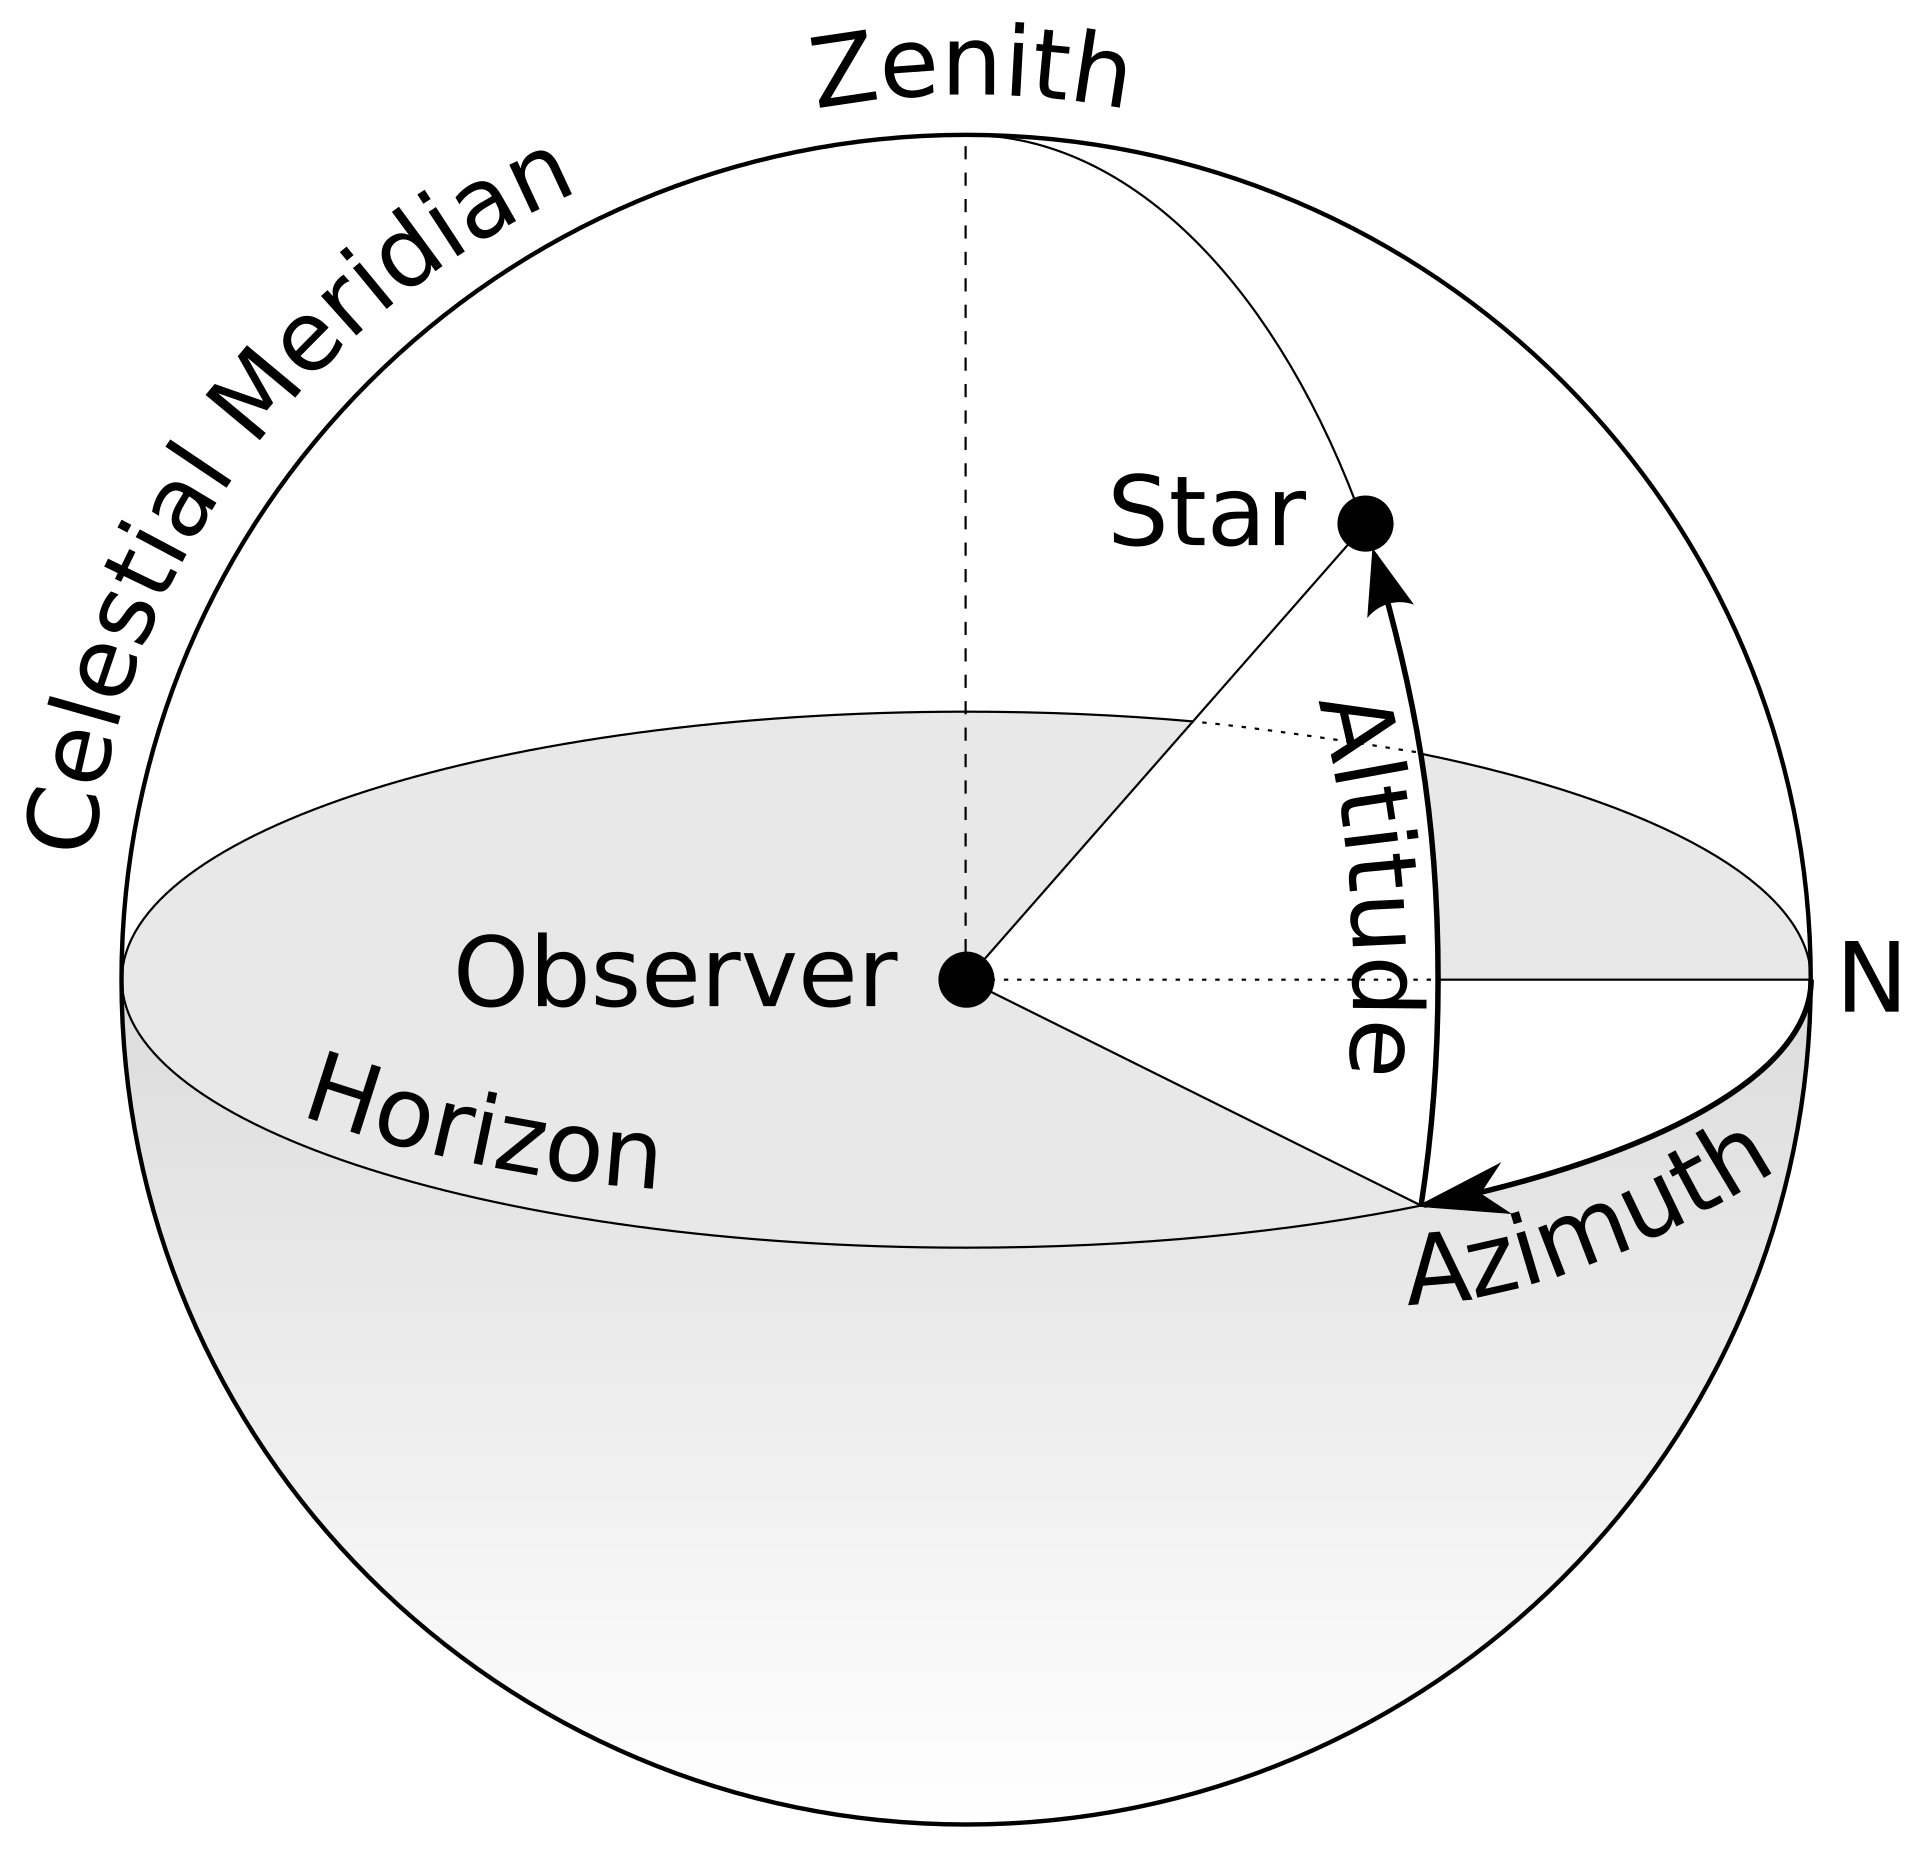
\includegraphics[width=0.98\textwidth]{Astronomy/Azimuth-Altitude_schematic.png}
    \caption{The altitude-azimuth coordinate system used at APEX. Source \cite{altaz_schematic}}
    \label{fig:altaz_coords}
\end{figure}




\section{Radio/(sub)-mm telescope basics}





\begin{figure}[H]
    \centering
    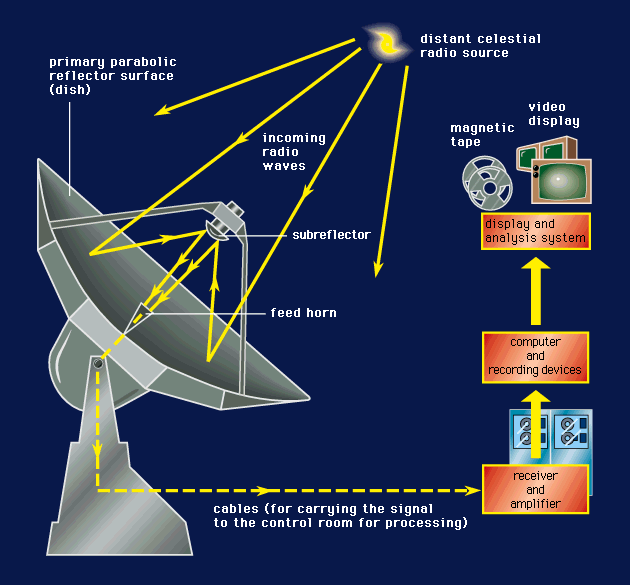
\includegraphics[width=0.98\textwidth]{Astronomy/radio_telescope.png}
    \caption{The main parts of a radio telescope.}
    \label{fig:radio_telescope}
\end{figure}


% \section{Problem description}
% \textcolor{red}{This section have to be fixed completely}
% A telescope makes high precision observations of objects located very far away from Earth.
% Because of this distance, small changes such as the deformation of mirrors due to temperature might impact the precision drastically.\cc{Claudia Cicone: Here you could explain that astronomical objects are observed as they were "projected" in 2D angular coordinates on the sky, and you could talk about astronomical coordinates (see Lecture 5 notes of my course AST2210 for some explanation and references)
% }
% Over time, these deformations have been observed and analyzed, and in order to counter this, a pointing model is made.
% \cc{Claudia Cicone: The need for a pointing model is relevant mainly to sub-mm telescopes that cannot take real-time images of what they are observing, and so the precision of the pointing direction must be known accurately before starting the observations.}
% The pointing model uses measurements from various instruments and is fitted to the observed offsets.
% The model is used for about a month, or until it start performing poorly.
% The variation in measurements are still too big using only this model, so pointing scans have to be made regularly to correct even more.
% A pointing scan is an observation of an object with known location.
% When doing this, the offset on this observation is then added on top of the pointing model.
% These corrections to azimuth and elevations are used for a couple of hours, until a new pointing scan is made.
% \cc{Claudia Cicone: Need to define azimuth and elevation first, see other comment above
% }
% Using this approach, pointing error is reduced to about $4$ arc seconds.\\

% The aim of this thesis is to investigate the possibility of using machine learning to increase the performance of the telescope, by improving pointing accuracy.
% This can be done in multiple ways.

% One possibility is to apply a pointing model on top of the current pointing model using machine learning, such that the average offset is reduced even more.
% Another possibility is investigating the use of machine learning models to aid such that a pointing scan doesn't have to be made as often.
% This will reduce the workload at the telescope. \\

\section{Pointing model}\label{sec:pt_model}
Since radio/(sub)-mm telescopes observe over an extended time, they need a pointing model to obtain sufficiently accurate pointings.
The flux of the brightest radio sources is also weaker than the atmospheric emission,
which means that the signal is often hidden in the noise and needs to be extracted using long integrations and modulation techniques.
Therefore, astronomers must know that the pointing is accurate before initiating a long integration on the source.

The pointing model at APEX consists of two steps, an analytical model and additional pointing corrections performed at regular intervals based on recently observed pointing offsets.
The analytical model consists of fitting a multiple terms to the many measurements of the pointing offset (difference between input coordinates and the observed coordinates of the source).
These terms can be geometric terms or terms related to, for example, metrology data.
The fitted terms are used for $1$-$2$ months and run in the background adjusting all input coordinates.
The additional pointing corrections are performed by astronomers every $1$-$2$ hours during the observations and before observing a new target.

These equations explain the resulting pointing

\begin{align}
    Az &= Az_\text{input} + \Delta Az_\text{analytical model} + \Delta Az_\text{correction} \\ 
    El &= El_\text{input} + \Delta El_\text{analytical model} + \Delta El_\text{correction}
\end{align}
Where the first terms, $Az_\text{input}$ and $El_\text{input}$, are the input coordinates.
The second terms $\Delta Az_\text{analytical model}$ and $\Delta El_\text{analytical model}$ are the adjustment made according to the analytical model.
Furthermore, the last terms, $\Delta Az_\text{correction}$ and $\Delta El_\text{correction}$, are the corrections based on recently measured pointing offsets.

In the following section, we introduce and explain the adjustments from the analytical model and pointing offsets. 


\subsection{Analytical Model}

Accurately measuring pointing offsets without a pointing model can be challenging as the error is typically larger than the beam size, causing the source to fall outside the beam. At APEX,
astronomers use an optical receiver mounted in the primary mirror to make the initial observations, which allows them to observe the source in real-time.
During this process, which the astronomers perform periodically every $1$-$2$ months, the telescope is pointed at various sources with known locations, yielding both input and observed coordinates.

The analytical pointing model at APEX considers various factors that affect pointing, including purely geometrical terms based on the imperfect mounting of telescope components and empirical terms.
It uses the terms described below, all of which are dependent on the azimuth $Az$ or elevation $El$, except for a couple of constant terms.
The coefficients for all the terms are determined by the \texttt{TPOINT} software, using a linear fit based on the observed offsets from a pointing campaign.
The sum of all terms is the adjustment made by the model.

Most of the terms described in this section are fitted on data collected from the optical receiver mounted in the primary mirror.
Then, the astronomers refine the terms using observations from different instruments to develop specialized pointing models for each, while most terms remain constant from the optical fit.
The analytical model is crucial in accurately determining the telescope's pointing offsets, essential in obtaining high-quality observational data.

The following descriptions of the terms are taken directly from the \texttt{TPOINT} software manual \cite{tpoint_manual}.

\subsubsection{Harmonic terms}
The analytical model has multiple harmonic terms, some geometrical and some empirical.
The \texttt{TPOINT} software used to develop the analytical model suggests terms that improve the model's performance on the chosen dataset.
The following terms are the empirical terms for azimuth.
\begin{align}
    \Delta Az =&  c_1 \cdot \sin{Az} + c_2 \cdot \frac{\cos{2Az}}{\cos{El}} + c_3 \cdot \cos{3Az} + c_4 \cdot \sin{2Az} \\
    &+ c_5 \cdot \cos{2Az} + c_6 \cdot \frac{\cos{Az}}{\cos{El}} + c_7 \cdot \frac{\cos{5Az}}{\cos{El}},
\end{align}
and the terms for elevation are

\begin{align}
    \Delta El =&  c_1 \cdot \sin{El} + c_2 \cdot \cos{El}+ c_3 \cdot \cos{2Az} + c_4 \cdot \sin{2Az} \\
    &+ c_5 \cdot \cos{3Az} + c_6 \cdot \sin{3Az} + c_7 \cdot \sin{4Az} + c_8 \cdot \sin{5Az}  
\end{align}


The \texttt{TPOINT} software denotes the harmonic terms in the format $Hrfci$. The list below explains the different terms.

\begin{itemize}
    \item $H$: Stands for harmonics
    \item $r$: The resulting variable, either $Az$ or $El$, denoting azimuth and elevation respectively.
    The resulting variable can also be $S$, which means the result is horizontal, or azimuth scaled by a factor $1/\cos{El}$.
    \item $f$: The harmonic function, either $S$ or $C$ denoting \textit{sine} and \textit{cosine}.
    \item $c$: The variable that the funciton $f$ is dependent on, either $Az$ or $El$.
    \item $i$: Integer value in the range $0$-$9$, denoting the frequency of the harmonic.
\end{itemize}

For example, is $\Delta Az = \text{HACA3}\cos{3Az}$ denoted as HACA3 in the \texttt{TPOINT} software.

\subsubsection{Az/El non-perpendicularity (NPAE)}
In an altazimuth mount, if the azimuth axis and elevation axis are not exactly at
right angles, horizontal shifts proportional to $\sin{El}$ occur. This effect is zero when pointing at the horizon and increases with elevation proportional to $1/\cos{El}$

\begin{equation}
    \Delta Az \simeq - \text{NPAE } \frac{\sin{El}}{\cos{El}}= - \text{NPAE } \tan{El},
\end{equation}
where NPAE is the horizontal displacement when pointing at Zenith.

\subsubsection{Horizontal displacement of Nasmyth rotator}
In a Nasmyth altazimuth mount, a horizontal displacement between the elevation axis of the mount and the rotation axis of the Nasmyth instrument-rotator produces
and image shift on the sky with a horizontal component
\begin{equation}
    \Delta Az \simeq - \text{NRX},
\end{equation}
and an elevation component
\begin{equation}
    \Delta El \simeq - \text{NRX} \sin{El},
\end{equation}
where NRX is the horizontal displacement.

\subsubsection{Left-right collimation error}
In an altazimuth mount, the collimation error is the non-perpendicularity between the nominated pointing direction and the elevation axis.
It produces a horizontal image shift given by
\begin{equation}\label{eq:pmodel_ca}
    \Delta Az \simeq -\text{CA} / \cos{El}
\end{equation}


\subsubsection{Azimuth and elevation index error}
Index errors are the errors when pointing at origo.

The azimuth index error is 
\begin{equation}
    \Delta Az = -\text{IA},
\end{equation}

and elevation index error is
\begin{equation}\label{eq:pmodel_ie}
    \Delta El = \text{IE}
\end{equation}

\subsubsection{Azimuth axis misalignment} 

In an altazimuth mount, misalignment of the azimuth axis north-south or east-west causes errors.
The errors caused by misalignment in the north-south are given by

\begin{equation}
    \Delta Az \simeq - \text{AN} \sin{Az} \cdot \tan{El},
\end{equation}

and

\begin{equation}
    \Delta El \simeq - \text{AN} \cos{Az},
\end{equation}
where AN is the misalignment alignment in the north-south direction.
The errors given by misalignment in east-west are given by

\begin{equation}
    \Delta Az \simeq - \text{AW} \cos{Az} \tan{El},
\end{equation}

and

\begin{equation}
    \Delta El \simeq \text{AW} \sin{Az},
\end{equation}
where AW is the misalignment alignment in the east-west direction.

\begin{table}[h]
    \centering
    \caption{The terms in the analytical model. \textcolor{red}{Table not complete.} }
    \begin{tabular}{cc}
    \textbf{Azimuth Terms} & \textbf{Elevation Terms} \\
    \hline
    \multicolumn{2}{c}{Optical observations} \\ 
    \cline{1-2}
    \hline
    $\sin{Az}$ & $\sin{El}$ \\
    $\cos{2Az}/\cos{El}$ & $\cos{El}$ \\
    $\cos{3Az}$ & $\cos{2Az}$ \\
    $\sin{2Az}$ & $\sin{2Az}$ \\
    $\cos{2Az}$     & $\cos{3Az}$ \\
    $\cos{Az}/\cos{El}$ & $\sin{3Az}$ \\
    $\cos{5Az}/\cos{El}$ & $\sin{4Az}$ \\
    & $\sin{5Az}$ \\
    \multicolumn{2}{c}{Radio receivers} \\
    \cline{1-2}
    \hline
    $\cos{Az}$ & $\cos{Az}$ \\
    \end{tabular}
\end{table}

\subsection{Pointing corrections} 
The analytical pointing model can only reduce the pointing offsets to about an average of \textcolor{red}{$x$ arcseconds}.
In order to reduce the pointing offsets even further, the astronomers at APEX update the pointing model by pointing at a source with known coordinates.
This operation is called a pointing scan, and by observing the resulting pointing offsets from the known source,
they update the terms CA and IE in the pointing model for azimuth and elevation correction, respectively
They update the terms as follows
\begin{align}
    \text{CA} &= \text{CA} + \delta_{\text{Az}} \label{eq:ca}\\ 
    \text{IE} &= \text{IE} - \delta_{\text{El}},\label{eq:ie},
\end{align}
where $\delta_{\text{Az}}$ and $\delta_{\text{El}}$ are the recently observed pointing offsets in azimuth and elevation, respectively.
The astronomers perform these pointing corrections every couple of hours to ensure the pointing is sufficient during science observations.

Note that we divide the term CA \eqref{eq:pmodel_ca} by cosine elevation, which converts the observed horizontal offset to azimuth.


\section{Research questions and related works} \label{sec:research_qs}
\begin{itemize}
    \item Reduce poitning offsets with machine learning model
    \item Replace analytical model with machine learning model
    \item reduce the frequency of pointing scans while maintaining pointing accuracy with machine learning model
\end{itemize}

\begin{itemize}
    \item Article about analytical model
    \item ...
\end{itemize}

\section{Database} \label{sec:database}


\subsection{Raw Data}
The raw data from the pointing scans using the NFLASH230 receiver provides input and actual coordinates.
They obtain the actual coordinates of the sources by combining the input coordinates with the adjustments made by the pointing model,
automatic adjustments based on sensory data, and the observed offset.
Then, they use this raw data to refine the model fit on data obtained from the optical receiver.
Table \ref{tab:raw_datanflash230} is included to provide an example of this data format. 


\begin{table}[h]
    \centering
    \caption{Extract of raw data obtained with NFLASH230. The data file also includes the source, which is irrelevant to this project.}
    \begin{tabular}{ccccc}
         & \multicolumn{2}{c}{Input} & \multicolumn{2}{c}{Observed} \\ 
        \cline{2-3} \cline{4-5}
        Date & Azimuth & Elevation & Azimuth & Elevation \\ 
        \hline
        2022-01-03 14:24:04 & $189.812879$ & $41.0762$ & $190.254779$ & $40.883651$ \\
        2022-01-03 18:59:40 & $50.842145$ & $73.371647$ & $51.269044$ & $73.203243$ \\
        2022-01-03 19:01:49 & $49.555916$ & $73.752182$ & $49.983112$ & $73.583545$ \\
        2022-01-03 19:16:10 & $39.378382$ & $76.076236$ & $39.781084$ & $75.908956$ \\
        2022-01-03 19:18:27 & $113.934309$ & $39.345667$ & $114.391232$ & $39.170168$ \\
        2022-01-22 13:54:31 & $94.04365$ & $18.148405$ & $94.492505$ & $17.981161$ \\
        2022-01-22 14:15:35 & $148.569964$ & $89.044036$ & $147.783271$ & $88.852306$ \\
        2022-01-22 14:18:15 & $215.664924$ & $49.563821$ & $216.104389$ & $49.386438$ \\
    \end{tabular}
    \label{tab:raw_datanflash230}
    \end{table}



\subsection{The Monitor Database}
The monitor database is critical in this project, providing valuable sensory data from within and outside the telescope.
In this section, we will explore the data contained within the monitor database and identify the most relevant variables to our purposes.
We got a copy of the database containing data from 01.01.2022 to 17.09.2022.

\paragraph{Azimuth and Elevation}
The database includes tables for the input azimuth and elevation, labeled COMMANDAZ and COMMANDEL.
These tables contain the raw coordinates before the pointing model has adjusted the pointing.

The database also includes tables for the actual azimuth and elevation, labeled ACTUALAZ and ACTUALEL.
These tables contain the coordinates obtained after applying the pointing model and automatic adjustments based on sensory data.

Finally, the database contains tables for the azimuth and elevation velocity, labeled ACTUALVELOCITYAZ and ACTUALVELOCITYEL.
These tables provide information on the velocity of the telescope during observations.

The frequency of these measurements is $6$ data points per minute.
Figure \ref{subfig:scan_az} show these measurements for the duration of a pointing scan, along with additional data points before and after the scan.


\paragraph{Temperature Measurements}
Multiple instruments located at different locations on the telescope measure the temperature and store the measurements in the database.
The tables that contain these measurements are labeled TEMPERATURE, TEMP1 through TEMP6, TEMP26 through TEMP28, and TILT1T. 
Figure \ref{fig:corr_temp} indicates that many of these measurements are highly correlated.
For example, TEMP1 through TEMP6 show a strong correlation $\geq 0.98$.
Similarly, TEMP26 through TEMP28 and TEMPERATURE are also highly correlated.
The frequencies of some of these measurements are different, and they may all be found in Table \ref{tab:data_frequency}.
Figure \ref{subfig:scan_temp1} and \ref{subfig:scan_tilt1t} show the measurements of TEMP1 and TILT1T respectively
for the duration of a pointing scan and additional data points before and after the scan.


\begin{figure}[H]
    \centering
    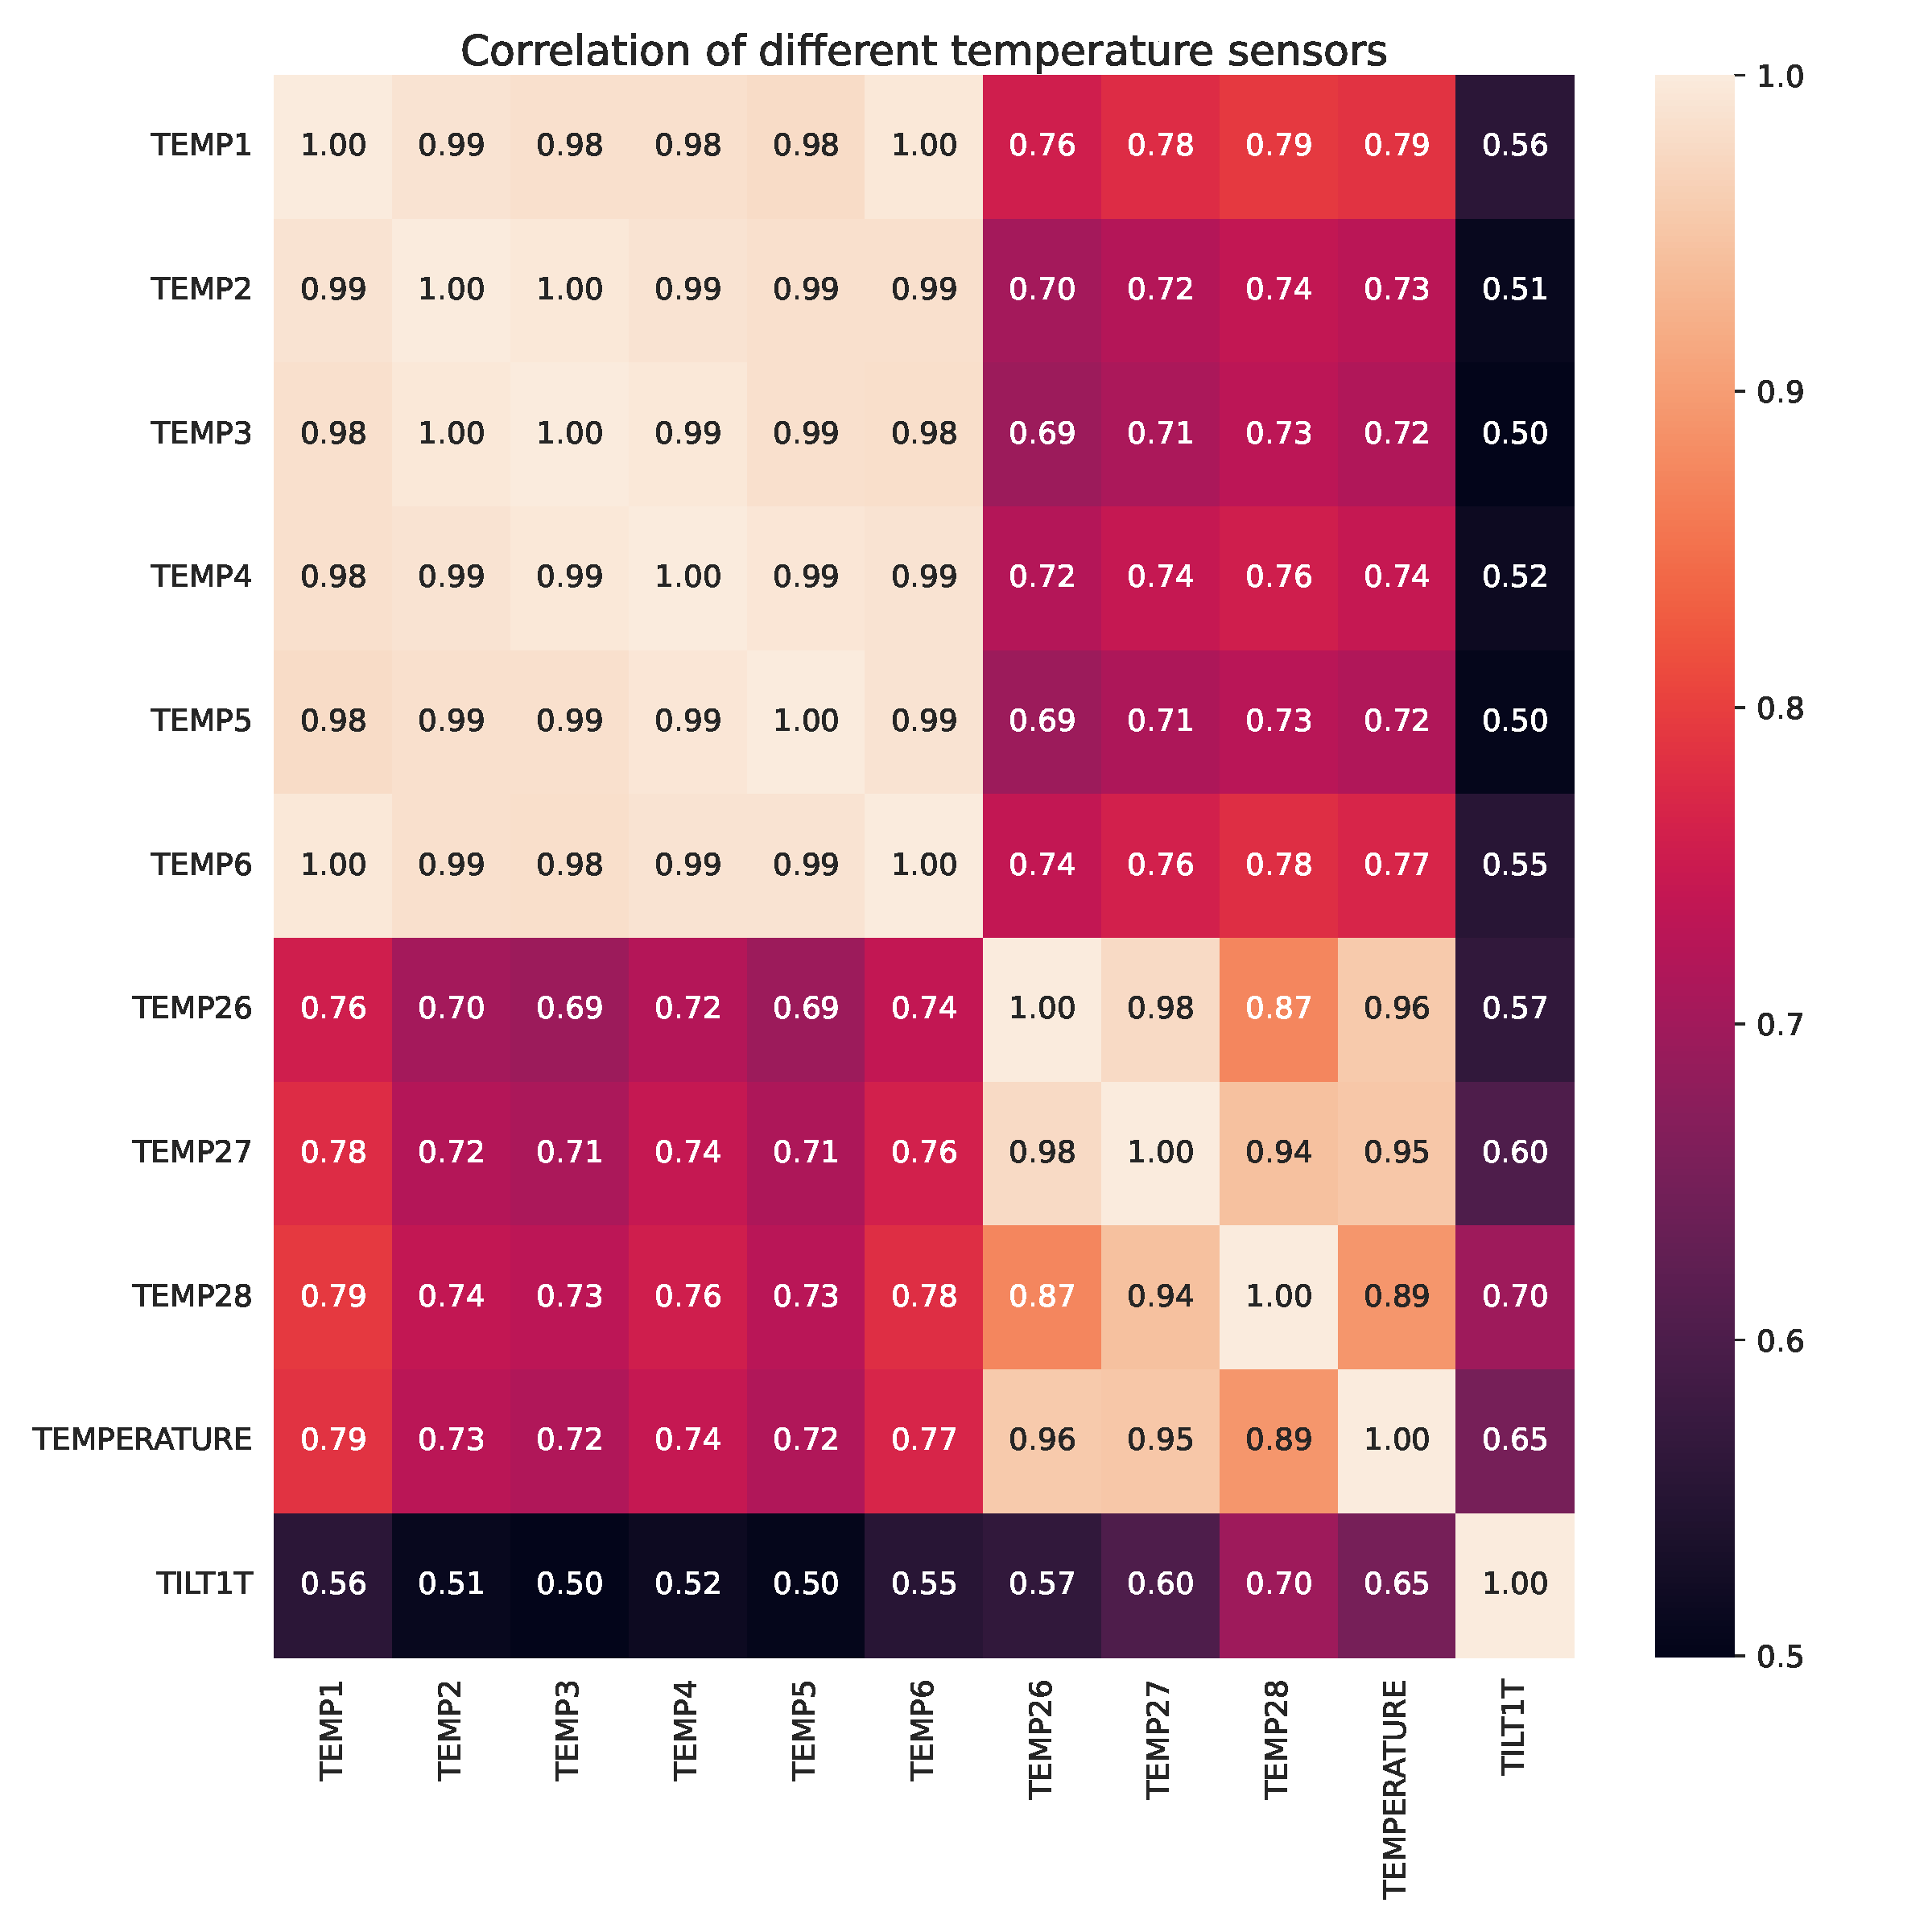
\includegraphics[width=0.98\textwidth]{Correlation/Correlation_temp.pdf}
    \caption{Linear correlation between temperature measures.
    The values are sampled by the median value at each pointing scan.}
    \label{fig:corr_temp}
\end{figure}

\paragraph{Hexapod}
The secondary mirror, also known as the subreflector, is supported by a hexapod.
The hexapod moves in three dimensions and rotates around azimuth and elevation axes.
There are five measures associated with the hexapod: POSITIONX, POSITIONY, POSITIONZ, ROTATIONX, and ROTATIONY.
These measures are essential for positioning the secondary mirror and ensuring accurate pointing. The frequency of these measurements is $6$ data points per minute.

\paragraph{Tiltmeter}
The telescope has two tiltmeters that measure its tilt or inclination to the vertical direction.
One tiltmeter aligns with the telescope's pointing, while the other is orthogonal.
They label these tiltmeters as TILT1X and TILT1Y, respectively, and they take measurements at a frequency of $12$ data points per minute.

\paragraph{Weather data}
The weather station at the telescope provides measurements of various weather parameters, including dew point, humidity, pressure, wind speed, and wind direction.
The instruments take measurements at a frequency of $5$ data points per minute.
The figures \ref{sub@subfig:scan_winddir} and \ref{subfig:scan_windspeed} show wind direction and speed measurements for the time period around a pointing scan.


\paragraph{Disp abs?}

Frequency of $12$ data points per minute.

\paragraph{Automatic adjustments}
Automatic adjustments based on readings from various sensors ensure accurate and stable pointing of the telescope.
These adjustments account for systematic errors previously modeled and are based on measurements from tiltmeters, temperature sensors installed at different locations, and other relevant data sources.
Some system at the telescope automatically makes these adjustments, and the tables in the database that contain information about these adjustments start with DAZ or DEL, denoting adjustments in azimuth and elevation, respectively.
The frequency of this data is $12$ data points per minute.
Table \ref{tab:data_frequency} shows a comprehensive list of these variables.

\paragraph{Data frequency}
The monitor database provides data with varying frequencies, as shown in Table \ref{tab:data_frequency},
which lists the approximate number of data points per minute for each table used in this project.

\begin{table}[H]
    \caption{The frequency in data points per minute of different variables in the monitor database.}
    \centering
    \begin{tabular}{lr}
        \toprule
        Table &  Frequency [datapoints/minute] \\
        \midrule
        ACTUALAZ &                    6 \\
        ACTUALEL &                    6 \\
        ACTUALVELOCITYAZ &                    6 \\
        ACTUALVELOCITYEL &                    6 \\
        COMMANDEL &                    6 \\
        COMMANDAZ &                    6 \\
        TILT1X &                   12 \\
        TILT2Y &                   12 \\
        TILT1T &                   12 \\
        TEMPERATURE &                    5 \\
        TEMP1 &                    6 \\
        TEMP2 &                    6 \\
        TEMP3 &                    6 \\
        TEMP4 &                    6 \\
        TEMP5 &                    6 \\
        TEMP6 &                    6 \\
        TEMP26 &                    2 \\
        TEMP27 &                    2 \\
        TEMP28 &                    2 \\
        DAZ\_TEMP &                   12 \\
        DAZ\_TILT &                   12 \\
        DAZ\_TILTTEMP &                   12 \\
        DAZ\_SPEM &                   12 \\
        DAZ\_DISP &                   12 \\
        DAZ\_TOTAL &                   12 \\
        DEL\_TEMP &                   12 \\
        DEL\_TILT &                   12 \\
        DEL\_TILTTEMP &                   12 \\
        DEL\_SPEM &                   12 \\
        DEL\_DISP &                   12 \\
        DEL\_TOTAL &                   12 \\
        POSITIONX &                    6 \\
        POSITIONY &                    6 \\
        POSITIONZ &                    6 \\
        ROTATIONX &                    6 \\
        ROTATIONY &                    6 \\
        DISP\_ABS1 &                   12 \\
        DISP\_ABS3 &                   12 \\
        DISP\_ABS2 &                   12 \\
        DEWPOINT &                    5 \\
        PRESSURE &                    5 \\
        HUMIDITY &                    5 \\
        WINDSPEED &                    5 \\
        WINDDIRECTION &                    5\\
        \bottomrule
    \end{tabular}
    \label{tab:data_frequency}
\end{table}


\begin{figure}[H]
    \centering
    \begin{subfigure}[t]{0.49\textwidth}
        \centering
        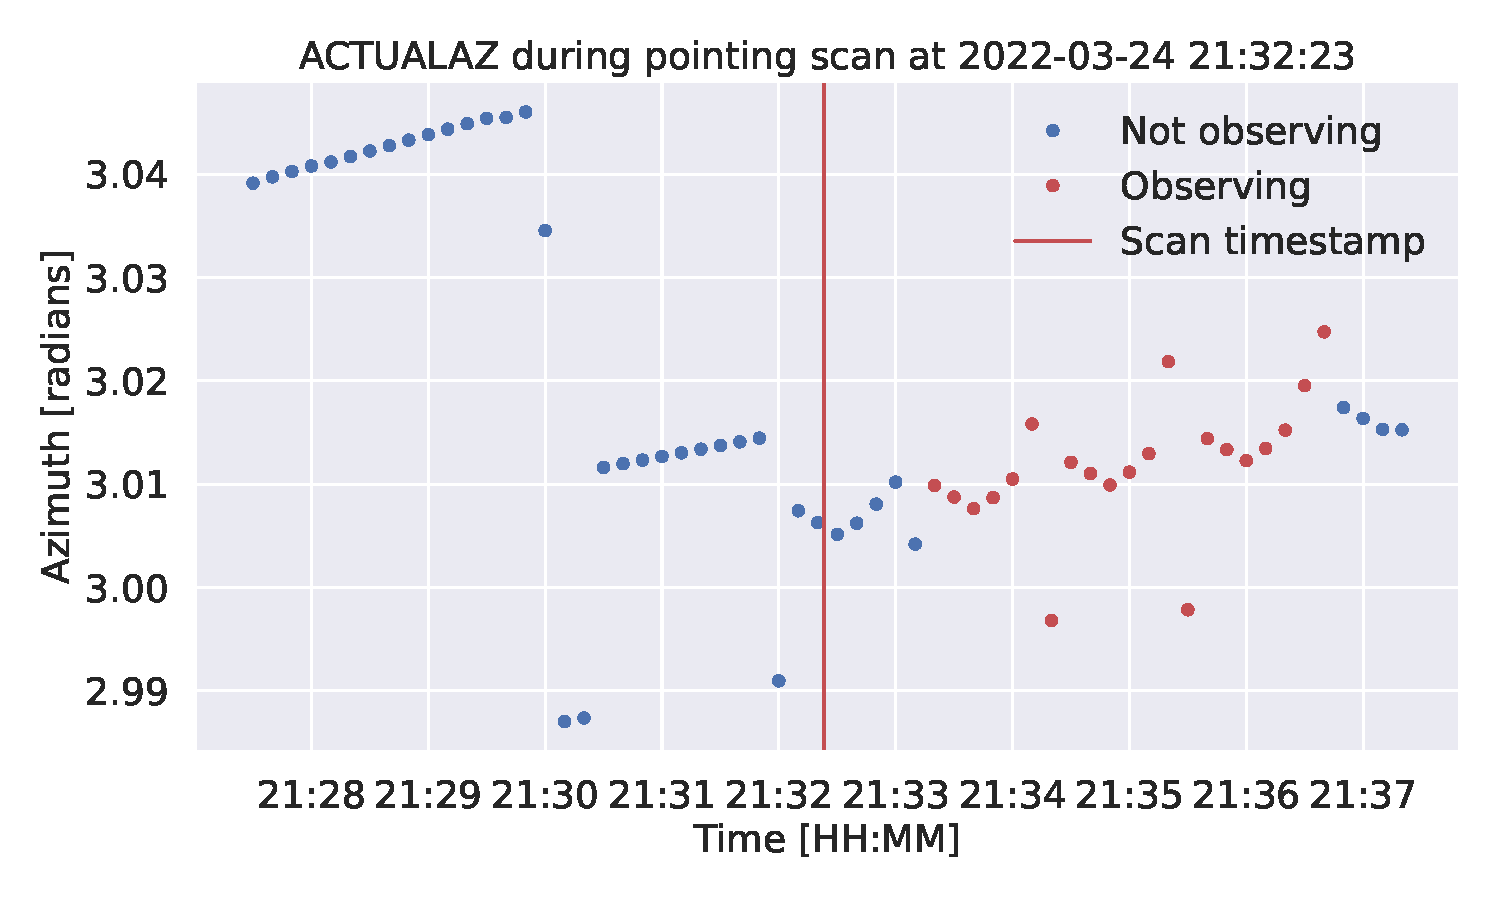
\includegraphics[width=\textwidth]{Feature during scans/scan_ACTUALAZ_335.pdf}
        \caption{Azimuth angle}
        \label{subfig:scan_az}
    \end{subfigure}
    \begin{subfigure}[t]{0.49\textwidth}
       \centering
       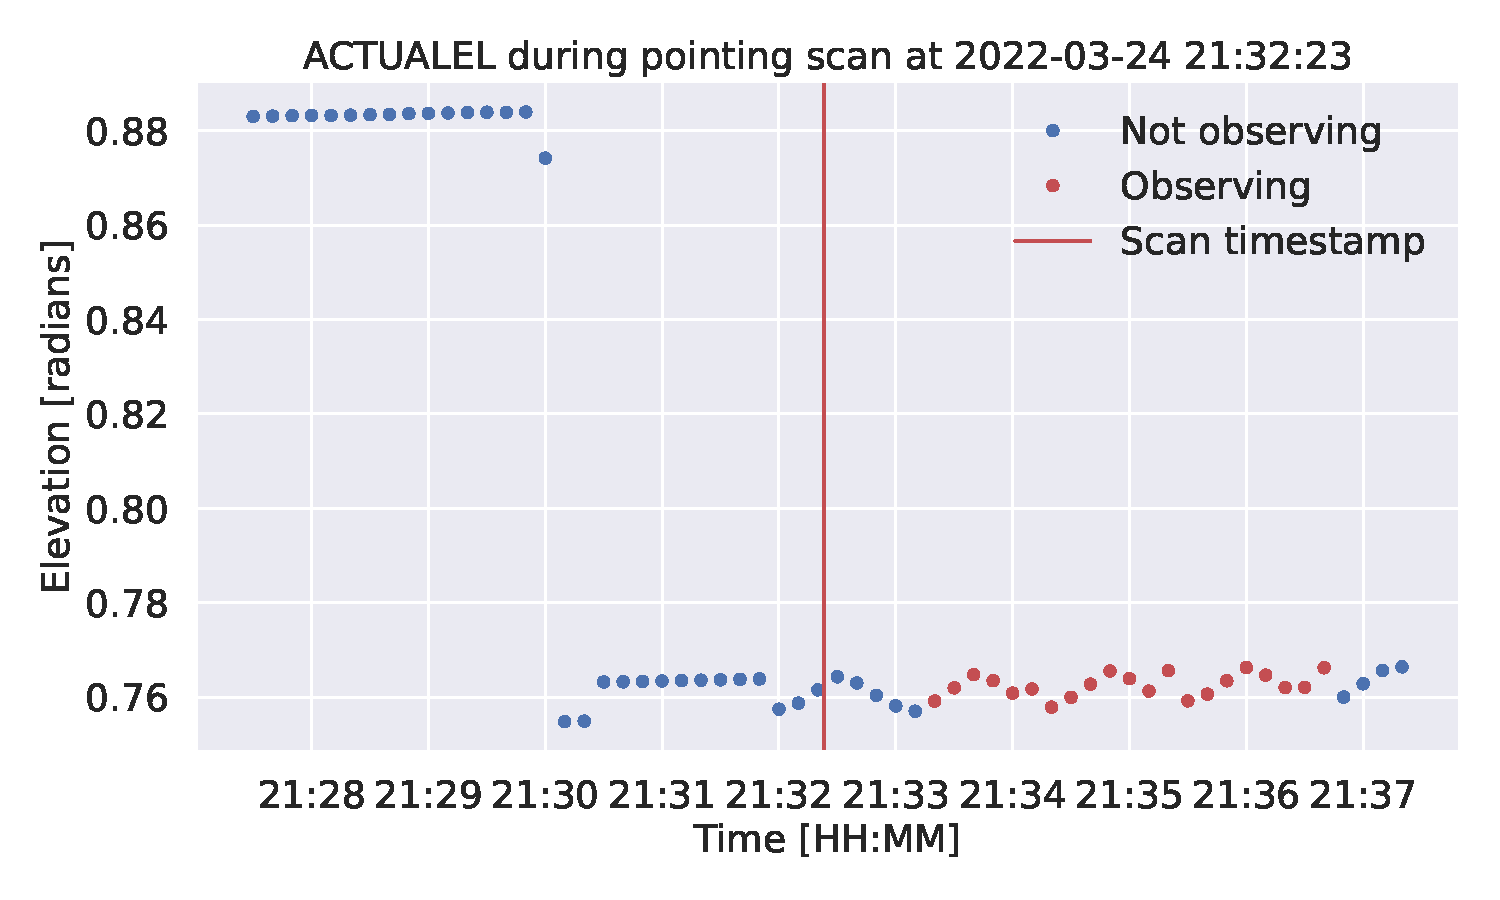
\includegraphics[width=1\textwidth]{Feature during scans/scan_ACTUALEL_335.pdf}
       \caption{Elevation angle.}
       \label{subfig:scan_el}
    \end{subfigure}
    \\~\\
    \begin{subfigure}[t]{0.49\textwidth}
        \centering
        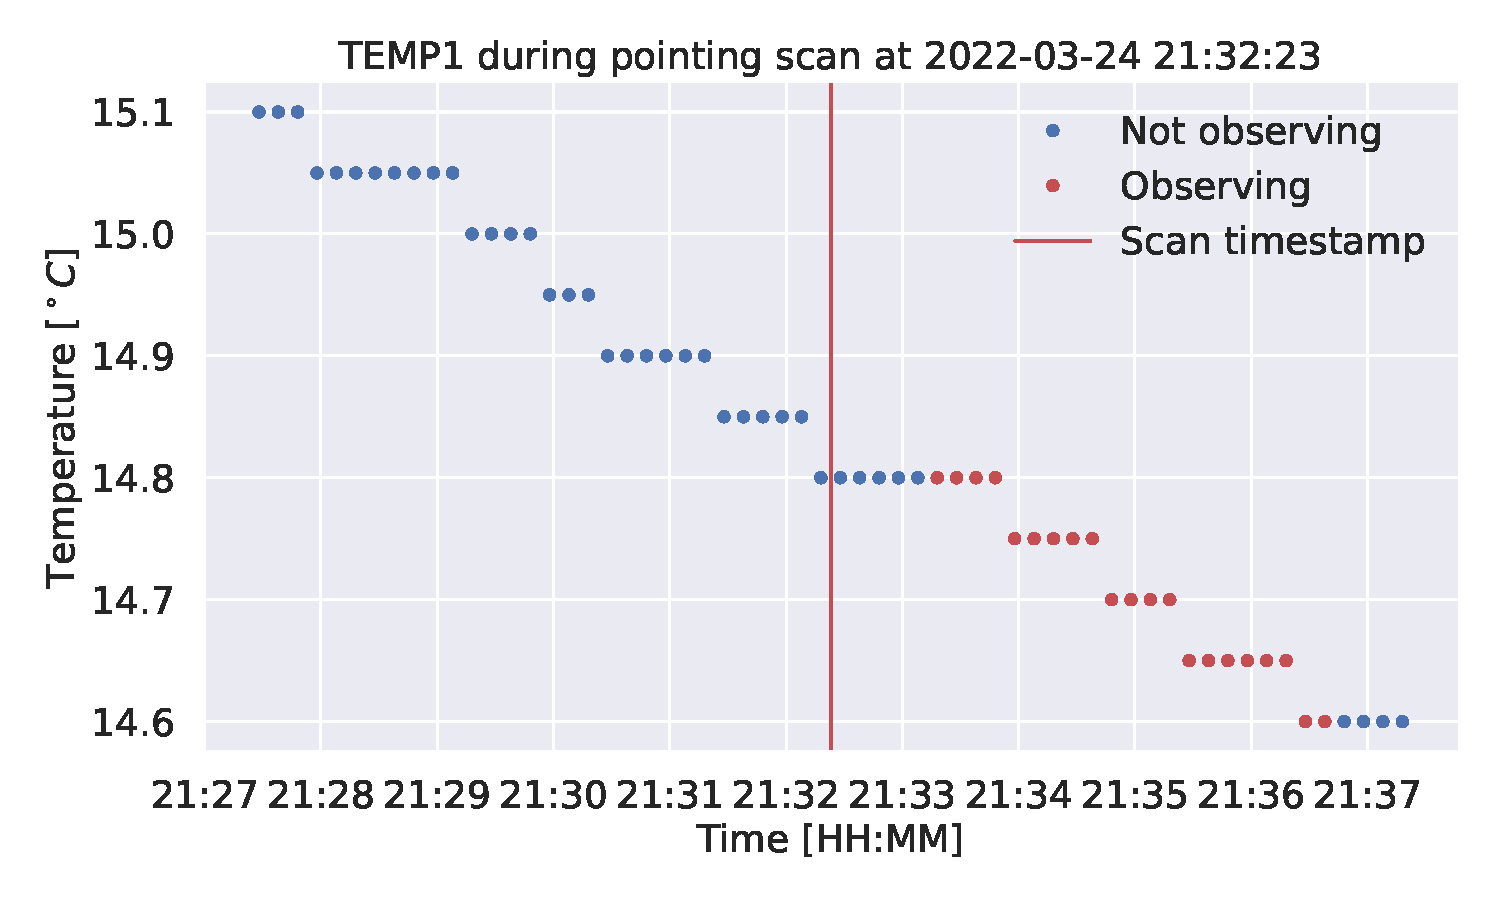
\includegraphics[width=\textwidth]{Feature during scans/scan_TEMP1_335.pdf}
        \caption{Temperature measurements at temperature sensor $1$.}
        \label{subfig:scan_temp1}
    \end{subfigure}
       \begin{subfigure}[t]{0.49\textwidth}
        \centering
        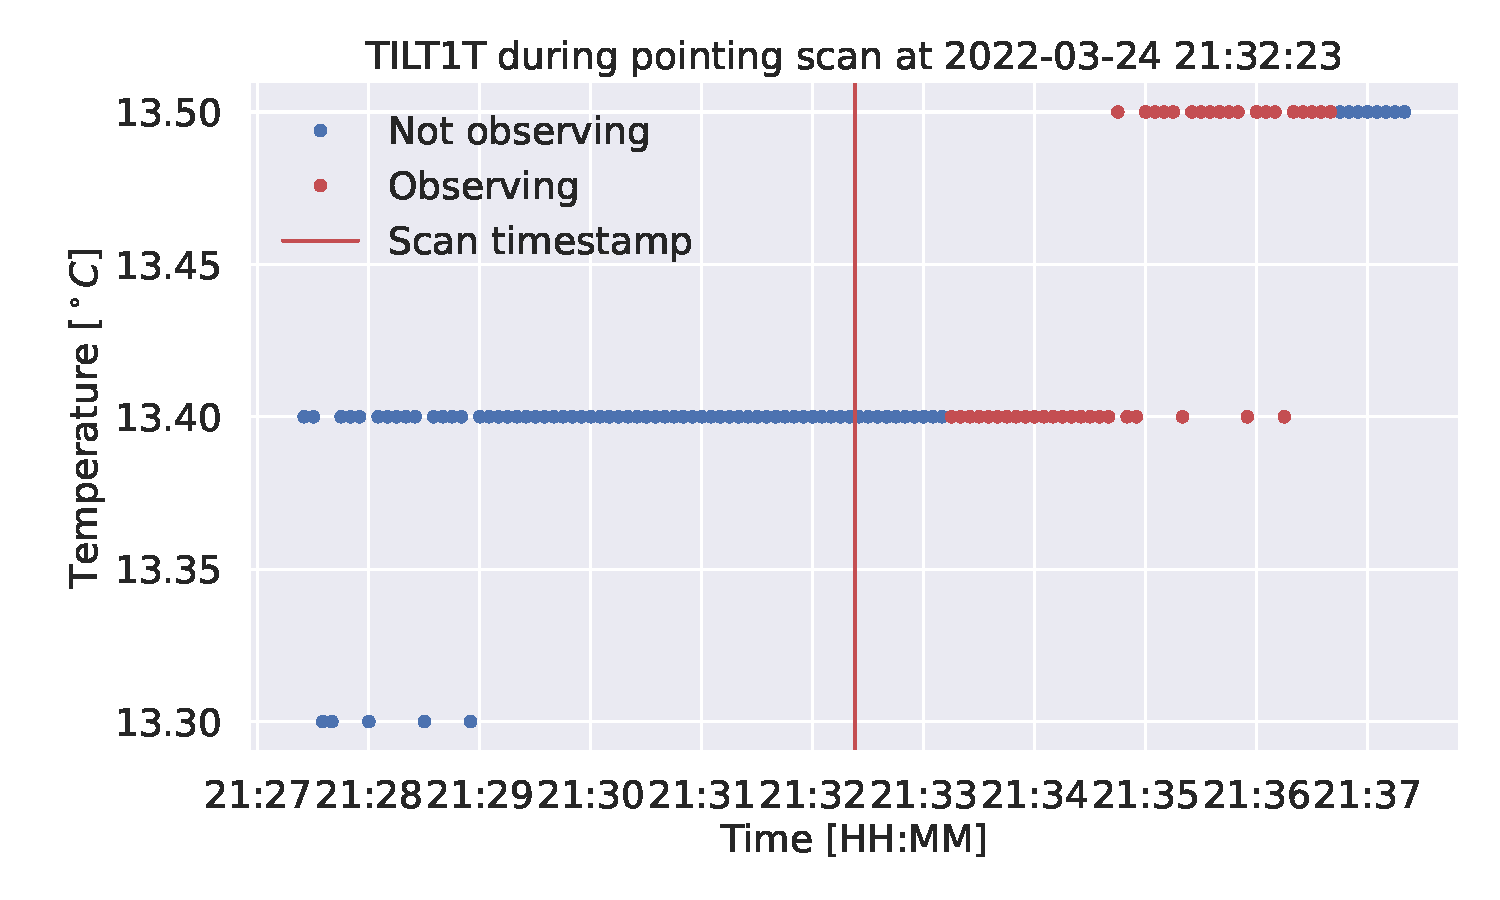
\includegraphics[width=\textwidth]{Feature during scans/scan_TILT1T_335.pdf}
        \caption{Temperature measurements at tiltmeter $1$.}
        \label{subfig:scan_tilt1t}
    \end{subfigure}
    \\~\\
    \begin{subfigure}[t]{0.49\textwidth}
        \centering
        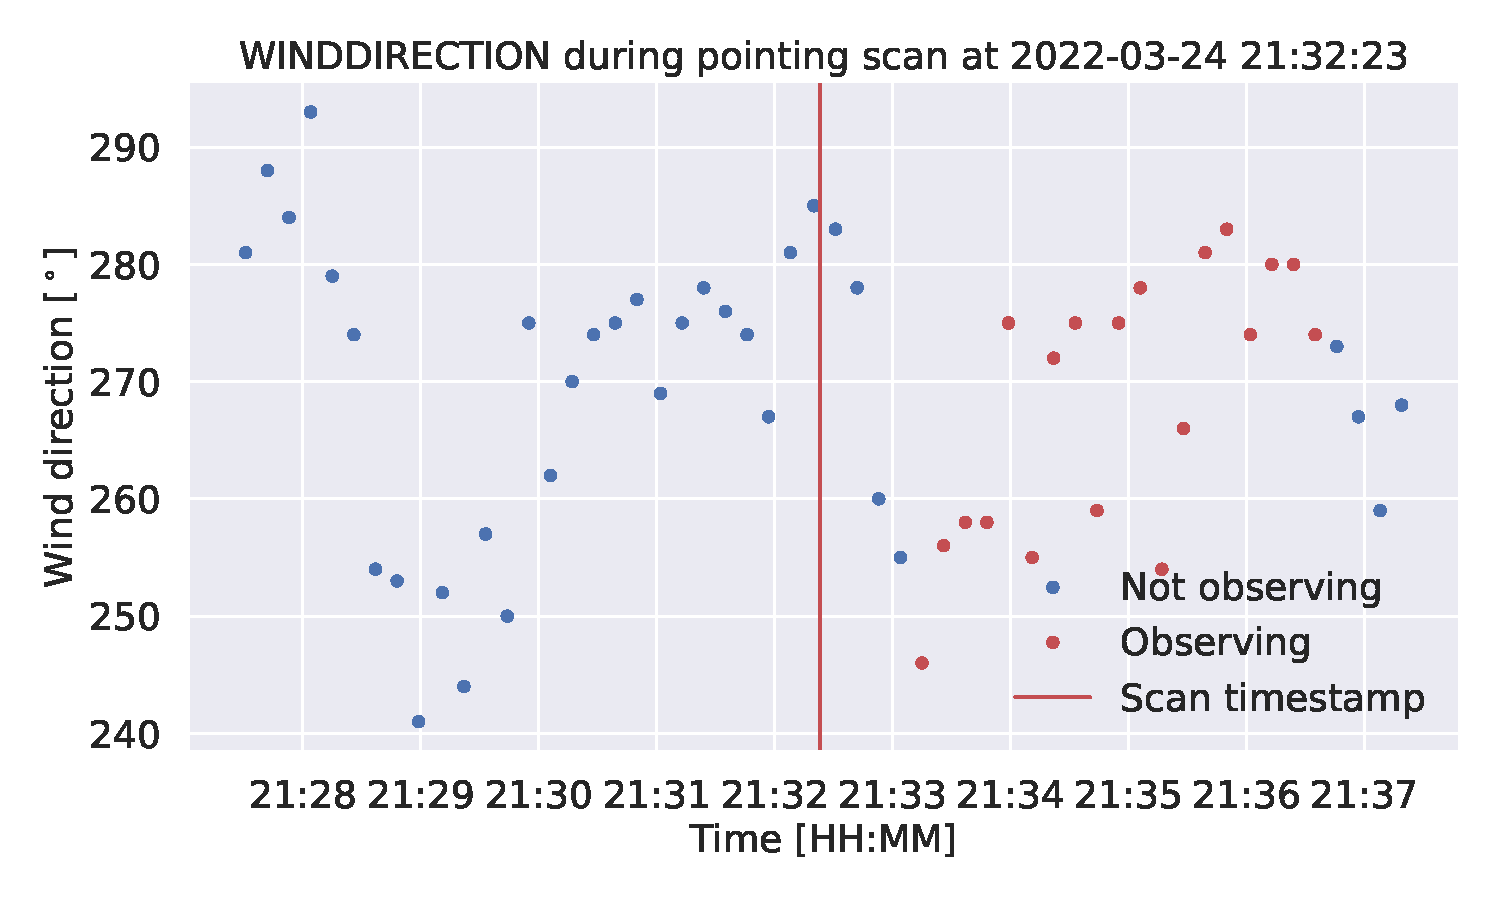
\includegraphics[width=\textwidth]{Feature during scans/scan_WINDDIRECTION_335.pdf}
        \caption{Wind direction data from the weather station, measured in degrees from North, where clockwise is the positive angle direction.}
        \label{subfig:scan_winddir}
    \end{subfigure}
       \begin{subfigure}[t]{0.49\textwidth}
        \centering
        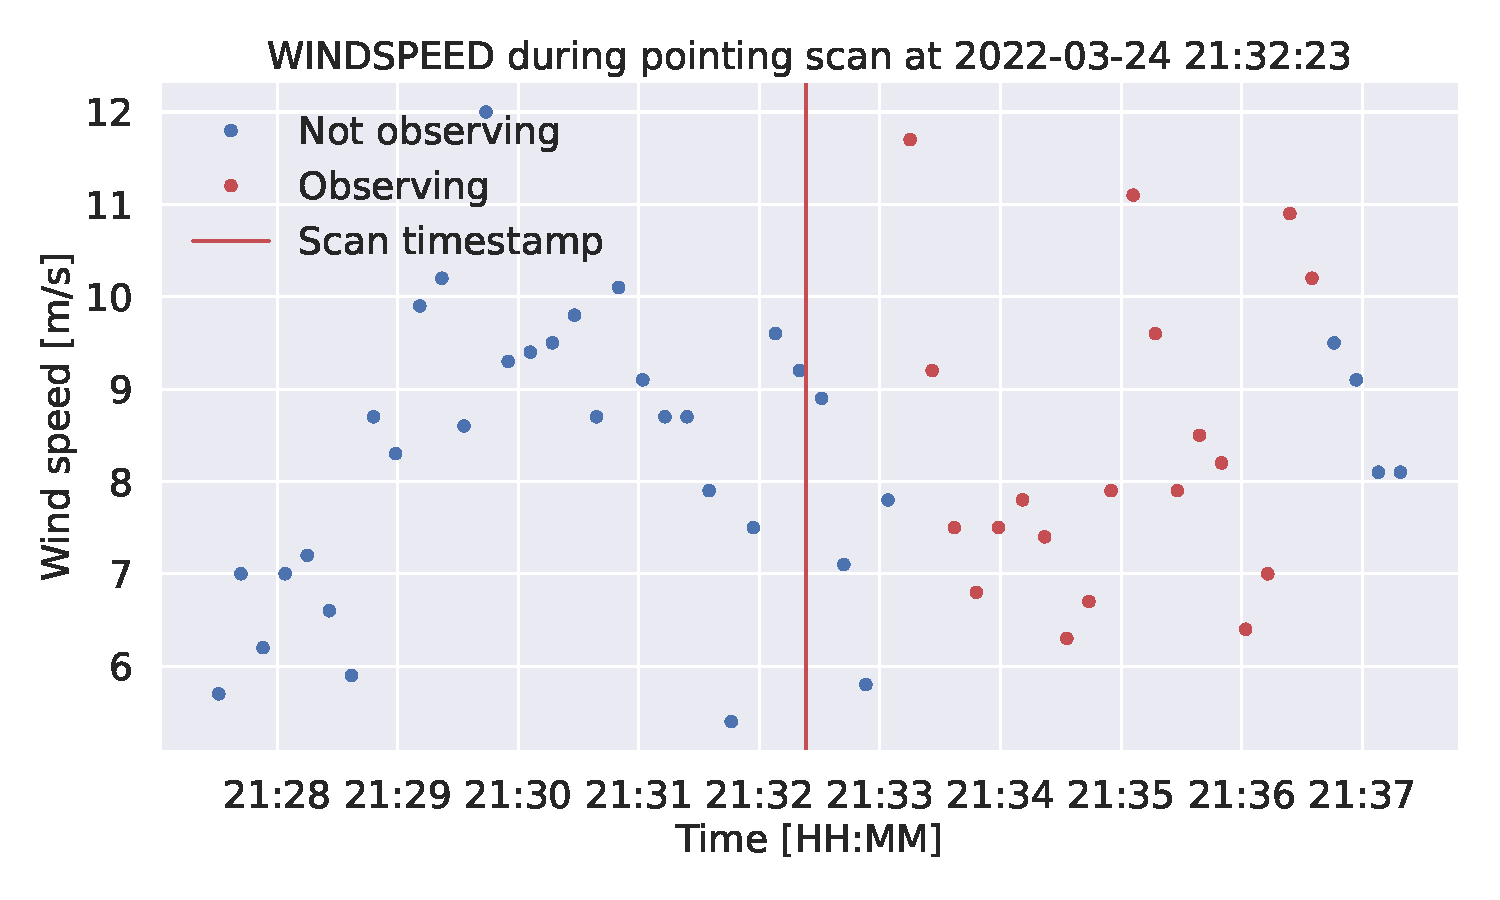
\includegraphics[width=\textwidth]{Feature during scans/scan_WINDSPEED_335.pdf}
        \caption{Wind speed data from the weather station.}
        \label{subfig:scan_windspeed}
    \end{subfigure}
     \caption{Scatter plots that show different sensory data from before, during, and after a pointing scan. The red line denotes the timestamp for a scan in the pointing scan database.
     The red dots indicate when the telescope is observing, while the blue dots indicate when the telescope is idle or preparing to observe.}
     \label{fig:features_during_scans}
\end{figure}


\subsection{Pointing scan data}
During a pointing scan, the telescope observes a source with a known location to obtain a pointing offset.
The observers use this offset to recalibrate the pointing model. There are two types of pointing scans: Line-pointings and continuum scans.
Figure \ref{fig:features_during_scans} shows the information in the monitor database from a pointing scan.

\paragraph{Line-pointing}
A line-pointing involves pointing at an extended source. 
The telescope then makes ten scans, recording the flux intensity from the source, five vertically and five horizontally,
around the center of the pointing, as shown in figure \ref{fig:line_pointings}.
The upper panel shows a high-quality pointing scan, and the lower panel shows a noisy, low-quality pointing scan.
The cross-plot on the right side shows the line spectrum for each observation (center plus eight offset observations).

The integrals of the flux recorded from the source are plotted as blue dots on the left-hand side of the panel.
A Gaussian is fitted to these points, and the table shows the resulting amplitude, full width at half maximum (FWHM), and offsets.

\begin{figure}[H]
    \centering
     \begin{subfigure}[b]{0.75\textwidth}
         \centering
         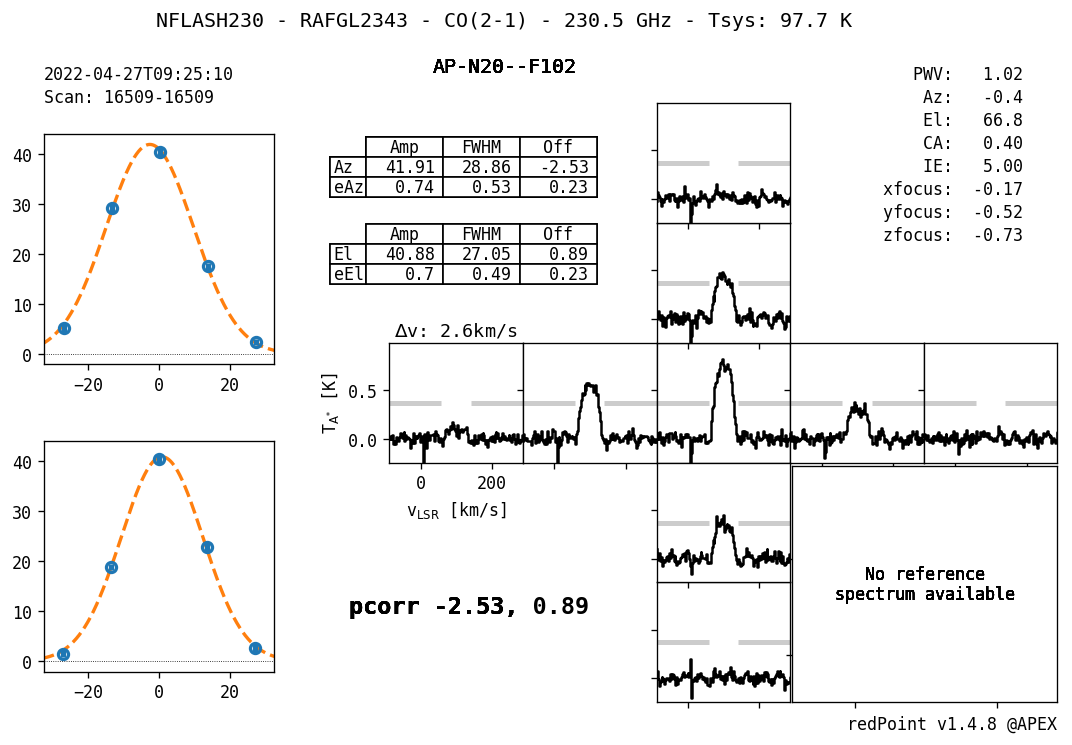
\includegraphics[width=\textwidth]{Pointing Scans/good_line.png}
         \caption{Line-pointing with little noise and a good Gaussian fit.}
         \label{subfig:good_line}
     \end{subfigure}
    \\
     \begin{subfigure}[b]{0.75\textwidth}
         \centering
         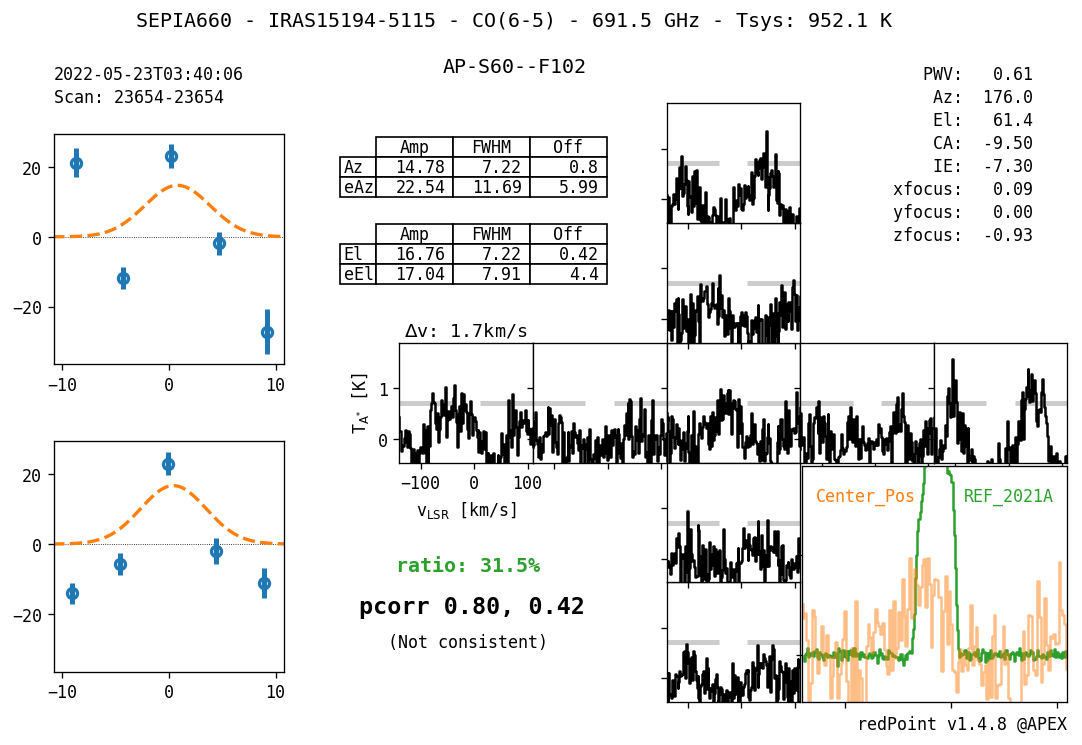
\includegraphics[width=\textwidth]{Pointing Scans/bad_line.png}
         \caption{Noisy line-pointing with bad Gaussian fit.}
         \label{subfig:bad_line}
     \end{subfigure}
    \caption{The two figures show line-pointing scans. a) is good and clean, and b) is noisy and unreliable. A Gaussian is fit both for the azimuth and elevation pointing.
    The table shows the amplitude, full width at half maximum (FWHM), offset, and the uncertainty of these measures, for azimuth and elevation.
    The figures also show the correction applied during the pointing ($ca$ and $ie$), along with other metrics.}
    \label{fig:line_pointings}
\end{figure}

\paragraph{Continuum Scan}
Not all sources have emission lines; for these sources, the telescope performs a continuum scan instead. In this case, a source is continuously scanned in azimuth and elevation while recording the flux intensity.
A Gaussian curve is fitted to the recorded flux intensity to determine the offsets, amplitude, and full width at half maximum (FWHM).
Figure \ref{fig:continueous_pointings} show examples of continuum scans and the corresponding Gaussian fits.

\begin{figure}[H]
    \centering
     \begin{subfigure}[b]{0.75\textwidth}
         \centering
         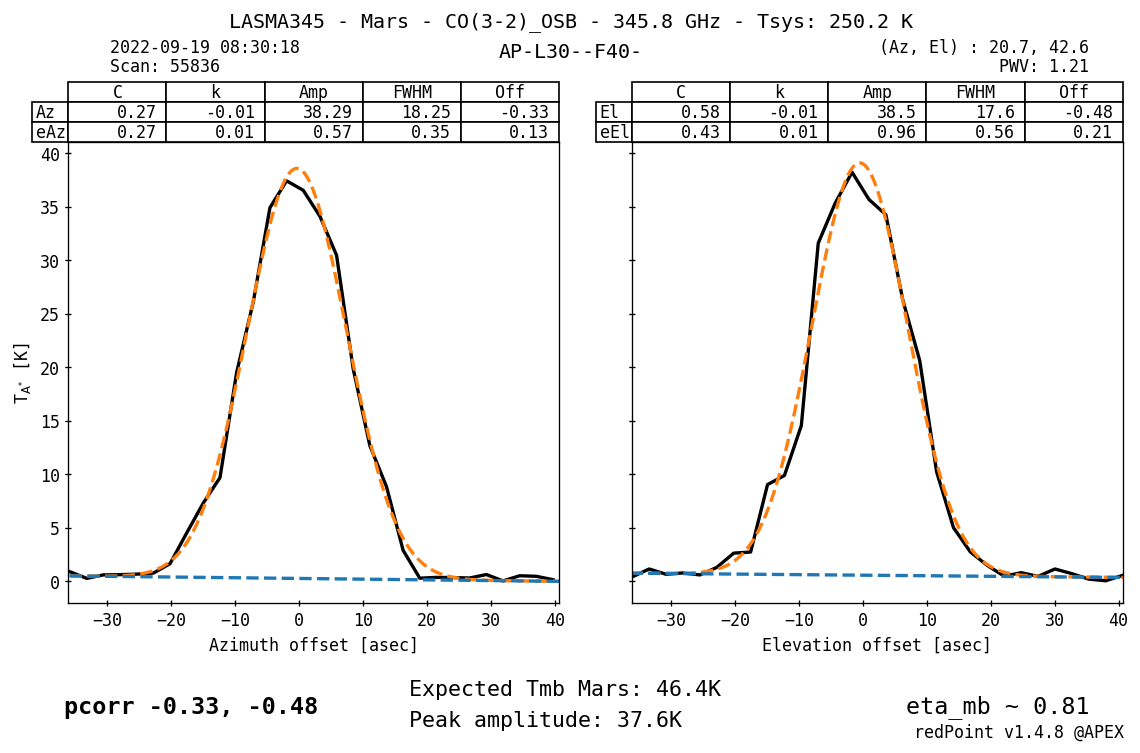
\includegraphics[width=\textwidth]{Pointing Scans/good_continuous.png}
         \caption{Line-pointing with little noise and a good Gaussian fit.}
         \label{subfig:good_continuous}
     \end{subfigure}
    \\
     \begin{subfigure}[b]{0.75\textwidth}
         \centering
         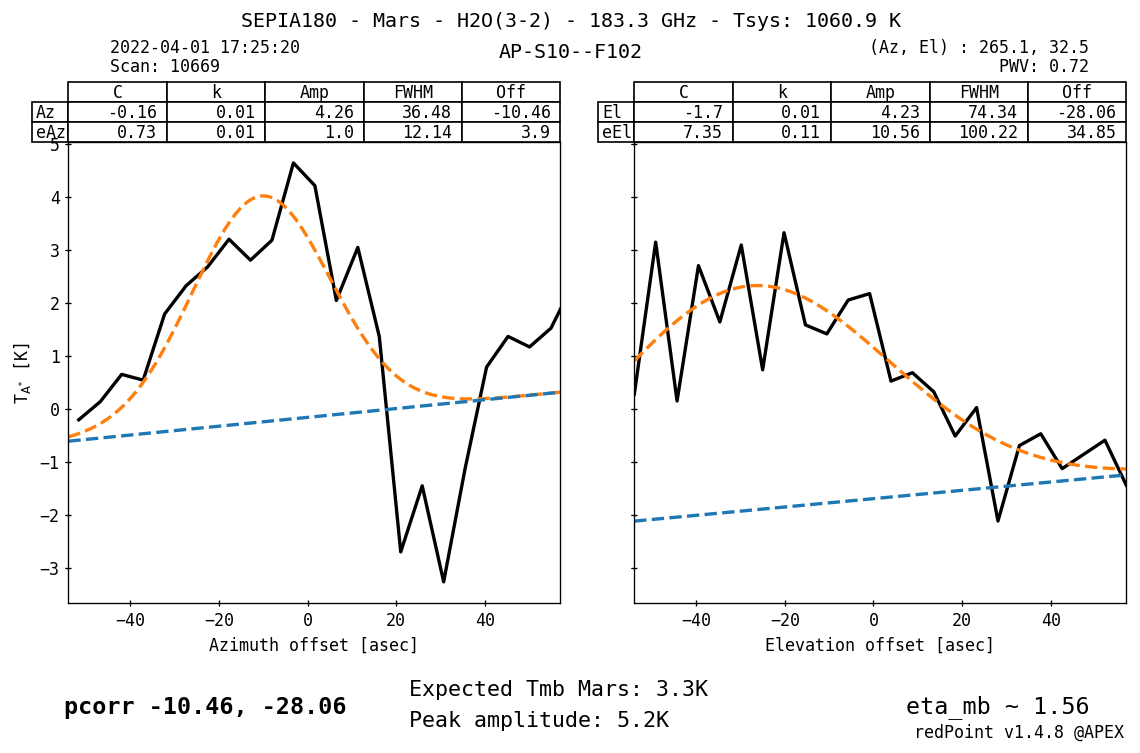
\includegraphics[width=\textwidth]{Pointing Scans/bad_continuous.png}
         \caption{Noisy line-pointing with bad Gaussian fit.}
         \label{subfig:bad_continuous}
     \end{subfigure}
    \caption{The two panels show continuum pointing scans. a) is good and clean, and b) is noisy and unreliable. A Gaussian is fit both for the azimuth and elevation pointing. The amplitude, full width at half maximum, offset, and the uncertainty of these measures are shown for both of the fits.}
    \label{fig:continueous_pointings}
\end{figure}



\paragraph{Pointing scan timestamp} 
In the main database, each pointing scan has a timestamp in the format YYYY-MM-DD HH:MM:SS, with a one-second resolution. This timestamp does not reflect the actual start of a pointing scan. Also, there is not information in the database itself that indicates whether the telescope is observing, but this information can be extracted from some dump files from the tiltmeter, which includes a flag indicating whether the telescope is idle, preparing to observe, or observing. Combining this flag with the timestamps, we can obtain the accurate start and end time of a pointing scan. However, these tiltmeter dump files are only available for some time periods.

\begin{itemize}
    \item Plots with scan times distribution
    \item proportion of scans we have the accurate time for
    \item What we did for hte other scans
    \item mention some deviation
\end{itemize}

\paragraph{Instruments}
The observing instruments on the telescope operate at various frequencies.
Table \ref{tab:instrument_usage} provides information on the frequency range covered by each instrument,
along with the number of scans performed using each instrument throughout the year 2022.\\

The broad range of frequencies at which astronomical phenomena emit electromagnetic radiation requires observation across a wide range of frequencies to study these phenomena comprehensively.
APEX's \href{https://www.eso.org/sci/facilities/apex/cfp/cfp110/instrument_summary.html.html}{website} provides a complete list of instruments along with their descriptions.
\begin{table}[H]
    \centering
    \caption{The number of times each instrument was used for a pointing scan in $2022$. There are $8847$ scans in total.}
    \begin{tabular}{lcr}
        \toprule
        Instrument & Frequency band [GHz] &\# of scans \\
        \midrule
        NFLASH230 & $200$-$270$ &3197 \\
        LASMA345  & $268$-$375$ &1861 \\
        NFLASH460 & $385$-$500$ &1394 \\
        SEPIA660  & $578$-$738$ & 856 \\
        SEPIA345  & $272$-$376$ & 818 \\
        SEPIA180  & $159$-$211$ & 359 \\
        HOLO      & - & 225 \\
        ZEUS2     & - & 103 \\
        CHAMP690  & - &  34 \\
        \bottomrule
        \end{tabular}
        \label{tab:instrument_usage}
\end{table}



\subsection{Tiltmeter dump files}
The tiltmeter dump files are a small part of the database and are only used to analyze when pointing scans start and end.
There are 280 of these files, and all have filenames in the format "Tiltmeter\_YYYY-MM-DD.dump," which indicates the data's date.
These files contain seven columns: datetime, azimuth, elevation, tilt1x, tilt1y, tilt1t, and the scan flag.
For our purpose, only the datetime and scan flags provide useful information.
Table \ref{tab:tiltmeter_example} shows an extract of the datetime and scan flag columns from one of the tiltmeter dumps.


\begin{table}[H]
    \centering
    \caption{Extract from a tiltmeter dump file.}
    \begin{tabular}{cc}
        \toprule
        Datetime & Scan flag \\
        \midrule
        2022-11-13T02:23:37 & IDLE \\
        2022-11-13T02:23:38 & IDLE \\
        2022-11-13T02:23:39 & PREPARING \\
        2022-11-13T02:23:40 & PREPARING \\
        $\vdots$ & $\vdots$ \\ 
        2022-11-13T02:23:52 & PREPARING \\
        2022-11-13T02:23:53 & PREPARING \\
        2022-11-13T02:23:55 & OBSERVING \\
        2022-11-13T02:23:56 & OBSERVING \\
        2022-11-13T02:23:57 & OBSERVING \\
        \bottomrule
    \end{tabular}
    \label{tab:tiltmeter_example}
\end{table}


\chapter{Machine Learning Background}
\section{Supervised learning} \label{sec:supervised_learning}
Supervised learning is a subfield of machine learning that refers to training a model to predict a specific target value based on input data.
In this context, we refer to the input data as "features." The training is supervised when paired with the corresponding target value for prediction.
There are two types of supervised learning, regression and classification. 
In regression, we predict a continuous variable, while in classification predict a binary value, true or false.
The model architecture of the model can be the same regardless of predicting a true/false or continuous value. 
The difference is in the loss function, which is used to evaluate the model's performance during training. The last layer activation function for neural networks is different for regression and classification. 
In-depth explanations of this will come in the following sections.

\section{Loss/Cost} \label{sec:loss_cost}
In machine learning, the loss of a model refers to the discrepancy between the predicted and true values.
It is calculated using a specific function designed to penalize incorrect predictions and measure the model's performance.
The ultimate goal of any machine learning model is to minimize the loss and thereby reduce the difference between predicted and desired outputs.
To achieve this, the model is trained by calculating the gradient of the loss function with respect to different components in the model.
These gradients determine how the model is adjusted to minimize the loss through an iterative process.
As a result, the model is optimized to make better predictions and achieve higher accuracy.\\

The most common loss function for regression is the mean squared error
\begin{equation} \label{eq:mse}
    \mathcal{L}(y, \Tilde{y}) = \frac{1}{N}\sum_{i=1}^N(y-\Tilde{y})^2,
\end{equation}
where $\tilde{y}$ is the prediction, $y$ the true value, and $N$ the number of predictions.

\subsection{Loss Functions}
Loss functions are used to evaluate the performance of the machine learning model during training.
We consider two different loss functions when predicting azimuth and elevation simultaneously with the same model, such as a neural network.
One loss function considers the offset in azimuth and elevation separately, and one considers the total distance.
Let $\Tilde{y}_{Az}$ and $\Tilde{y}_{El}$ denote the prediction for the offset in azimuth and elevation, respectively.
$y_{Az}$ and $y_{El}$ are the true values.
The first loss function is the mean squared error 
\begin{equation}\label{eq:mse1}
    \mathcal{L}_{\text{MSE}} = \frac{1}{2N}\sum_i^N \left( (y_{Az,i}-\Tilde{y}_{Az,i})^2 + (y_{El,i}-\Tilde{y}_{El,i})^2 \right),
\end{equation}
where $N$ is the number of predictions. 
\\
For the second loss function, we use the mean squared distance
\begin{equation}\label{eq:totaloff}
    \mathcal{L}_{\text{MSD}} = \frac{1}{N}\sum_i^N \left[ (y_{Az,i}-\Tilde{y}_{Az,i})^2 + (y_{El,i}-\Tilde{y}_{El,i})^2 \right],
\end{equation}
It is difficult to predict the effects of these loss functions if any at all, but one difference could be that $\mathcal{L}_{\text{MSE}}$ is more sensitive to outliers,
and $\mathcal{L}_{\text{MSD}}$ reduces the offsets more evenly. \\

For models with a single output azimuth or elevation, we use the regular mean squared error \eqref{eq:mse}

\section{Train/test set}
Machine learning models can be highly complex and fit all the data points in a dataset.
While this can result in perfect predictions on the training data, it often leads to poor performance on new data, a phenomenon known as overfitting.
To counteract this, the data is typically split into two parts - a training set and a validation set.
The model is trained on the training set, and the error on the validation set is used to evaluate the model's performance. 
By using a separate set of data for validation, we can better estimate the model's performance on new data and avoid overfitting.

When the error on the training data is low, the model has low bias.
However, if the model is too complex, it may also have high variance, meaning that it is overly sensitive to the training data and unable to generalize well to new data.
A model with high variance may perform well on the training data, but its performance on new data may be poor.
The key to building a good model is to balance bias and variance and to find the right level of complexity that will allow the model to generalize well.
Proper selection of the train/test split ratio and other techniques, such as regularization, can help achieve this balance and improve the model's performance.

One usually picks the machine learning model with the best performance on the validation set, but this performance is not a reasonable estimate of the expected performance on future predictions.
That is because many models are usually trained, and the model with the best performance on the validation set could have gotten lucky.
Therefore, a third test set is used to get an unbiased estimate of the model's performance.
The data in the test set is not used when training or validating and is only used to estimate the final model's performance.


\section{Scaling}
In machine learning, some models, such as neural networks, are highly sensitive to the scale of input data.
The inputs to a model often contain different types of data with varying scales.
Neural networks use weights to transform the input data, and each neuron in a fully connected network receives data from every input feature.
If the input features have different scales, training the weights can be slow and unstable.
Scaling the input data to have the same scale improves the speed and performance of the model.
In contrast, tree-based models are not affected by the range scale of the data since they consist of tests and not mathematical operations.

The most common scaling method is to standardize the data to have zero mean and a standard deviation of one. This is achieved by subtracting the mean and dividing by the standard deviation.
Mathematically, the standardization of a feature $x$ is represented as:

\begin{equation}
x_{scaled} = \frac{x - \mu}{\sigma}
\end{equation}

where $\mu$ is the mean of the feature values, and $\sigma$ is the standard deviation of the feature values.
The mean and standard deviation are computed using the following equations:

\begin{align}
\mu &= \frac{1}{n}\sum_{i=1}^{n}x_i\\
\sigma &= \sqrt{\frac{1}{n}\sum_{i=1}^{n}(x_i - \mu)^2},
\end{align}
where $n$ is the number of observations of the feature.
In addition to standardization, other scaling methods, such as min-max and robust scaling, are also used in specific cases.
Overall, scaling is a crucial step in preprocessing data for machine learning, as it can significantly impact the performance of a model.
However, for tree-based methods, scaling has no effect, as predictions are made based on conditions in the data, not mathematical operations.


\section{Decision Trees}
Decision trees are tree-like models that make decisions based on conditions.
As shown in Figure \ref{fig:decitiontree}, each circle represents a node with various types, including decision nodes that split into two other nodes and leaf/terminal nodes that do not.
The root node is the topmost decision node.
Given an observation, a single path to a leaf node represents the prediction made by the decision tree.

Trees are constructed greedily from the top, meaning that each split is made to minimize the loss function at the current step without considering future splits.
More than a single decision tree is required for complex problems.
Various methods exist to improve decision tree models, as Figure \ref{fig:evolution_of_xgb} demonstrates.
The final step in the figure is XGBoost (Extreme Gradient Boost), a highly efficient and high-performing machine learning algorithm.
This section will briefly cover the methods used to optimize decision trees for prediction.
\cite{Mehta_2019}


\paragraph{Bagging}
Bagging, also known as Bootstrap Aggregation, is a method for training an ensemble of models that contribute to the final prediction.
Each model is trained using bootstrapped data (resampled from the original dataset with replacement), resulting in diverse decision trees.
The final prediction is the average of all ensemble models.

\paragraph{Random Forest}
Random forest is based on bagging, where each tree in the ensemble is made using only a randomly chosen subset of features.
This often leads to better generalization and reduced overfitting.

\paragraph{Boosting}
In boosting, an ensemble is created, but the trees are not made independently.
They are trained one by one, considering the previous trees.
A sample weight is assigned to each sample used to train a tree based on the current ensemble's accuracy.
Samples with significant prediction errors are assigned larger weights, and those with accurate predictions are assigned lower weights.
The final prediction is a weighted sum of all ensemble predictions, with weights based on each tree's accuracy.

\paragraph{Gradient Boosting}
Like in regular boosting, an ensemble of trees is created iteratively by considering the errors made by previous trees.
The process starts with a constant model that predicts the mean of all samples.
The gradient of the loss function with respect to each sample is calculated, and a tree is made to predict these gradients.
The new prediction is the constant plus a small step in the direction of the predicted gradients.
Repeated iteration with small steps in the gradient direction helps reduce both bias and variance.




\begin{figure}[H]
    \centering
    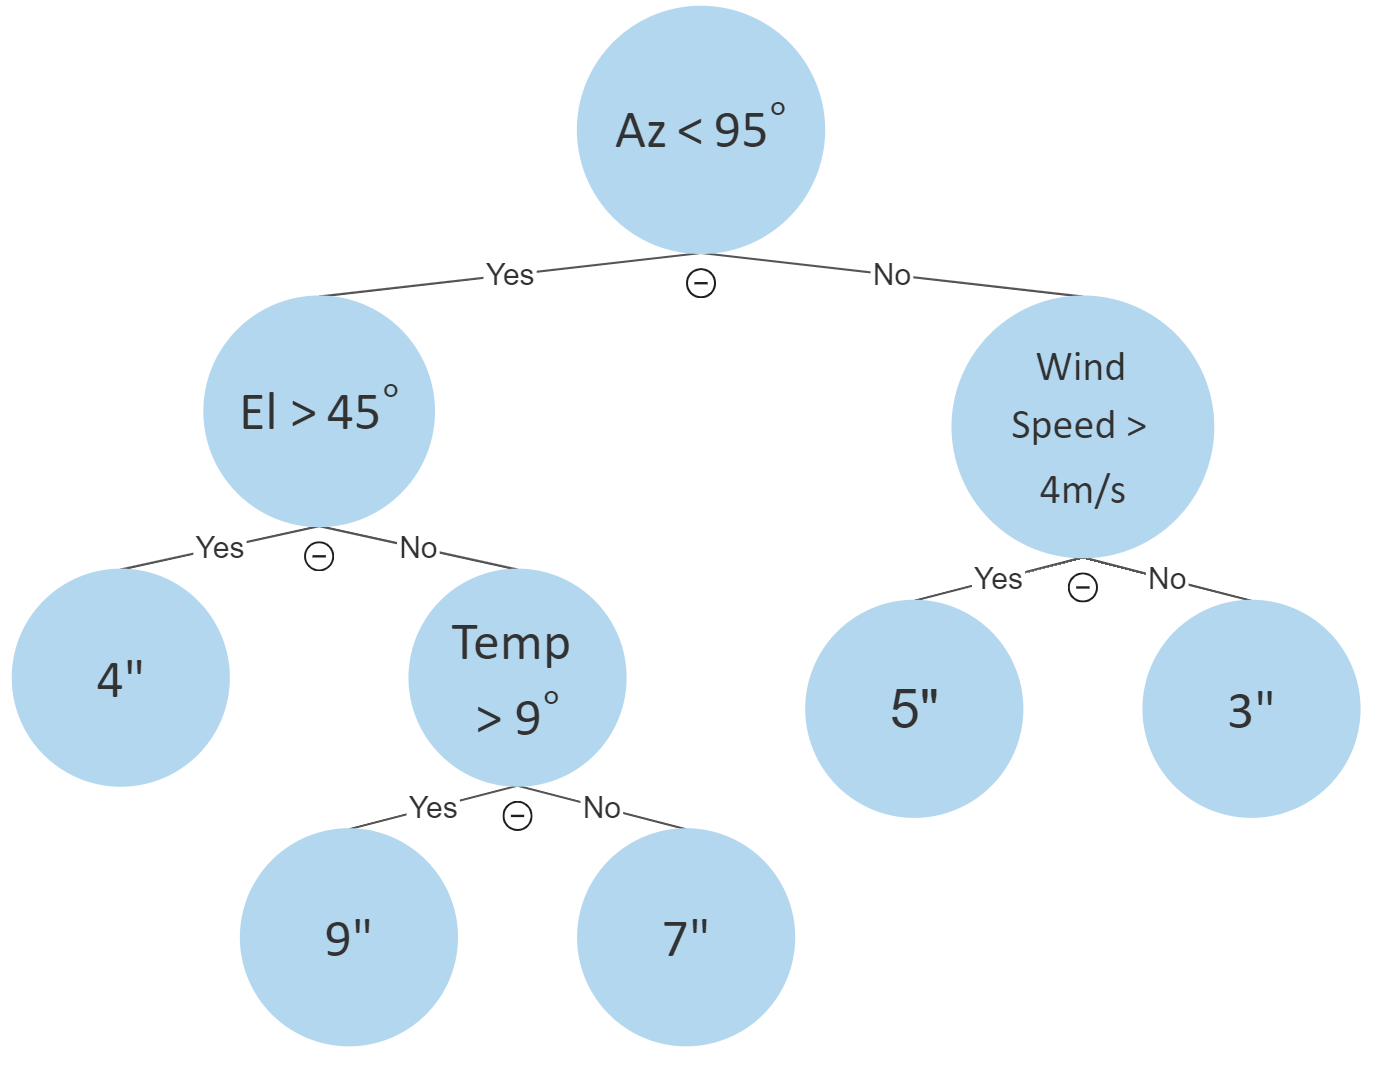
\includegraphics[width=0.98\textwidth]{Other figures/decisiontree_example.PNG}
    \caption{Decision tree with 3 decision nodes and 5 leaf nodes.}
    \label{fig:decitiontree}
\end{figure}

\begin{figure}[H]
    \centering
    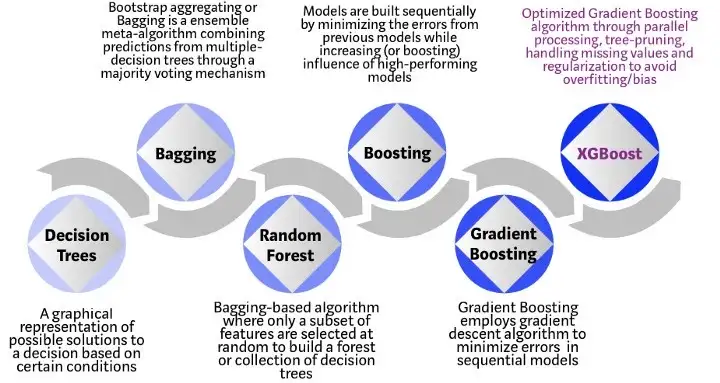
\includegraphics[width=0.98\textwidth]{Other figures/evolution_of_xgb.png}
    \caption{Evolution of XGBoost.
\cite{morde_vishal_nodate}}
    \label{fig:evolution_of_xgb}
\end{figure}

\section{Neural Networks}
A Neural Network (NN) is an Artificial Intelligence (AI) model composed of interconnected neurons inspired by biological neural networks in animal brains.
These networks are arranged in layers, as shown in Figure \ref{fig:nnfig}, and consist of an input layer, one or more hidden layers, and an output layer.
The size of the hidden layer(s) varies depending on the nature of the problem.
A neural network processes input to produce an output, ideally close to the true value.

Each connection in an NN has a trainable weight $w_{jk}^l$, representing the weight from the $k^{th}$ neuron in layer $(l-1)$ to the $j^{th}$ neuron in layer $l$.
Each neuron also has its own bias $b_j$, added to its output to prevent the input to its activation function $\sigma$ from being zero.
The activation function $\sigma$ applied to the neuron's output is the final transformation before passing data to the next layer.
This nonlinear function is crucial in allowing NNs to learn nonlinear relationships in data \cite{universal_approximation}.

The following is the mathematical explanation of how a neuron processes the outputs from the previous layer.

\begin{equation} \label{eq:act_neuron}
    a_{j}^l = \sigma\left(\sum_k w_{jk}^l a^{l-1}_k+b_j^l \right) = \sigma(z_j^l)
\end{equation}
The quantity 
\begin{equation}\label{eq:z_neuron}
    z_j^l = \sum_{k} w_{jk}^l a^{l-1}_k+b_j^l
\end{equation}
will be helpful when explaining how to optimize a neural network and can be considered the weighted input for neuron $j$ in layer $l$.


\begin{figure}[H]
    \centering
    % NEURAL NETWORK activation
% https://www.youtube.com/watch?v=aircAruvnKk&list=PLZHQObOWTQDNU6R1_67000Dx_ZCJB-3pi&index=1
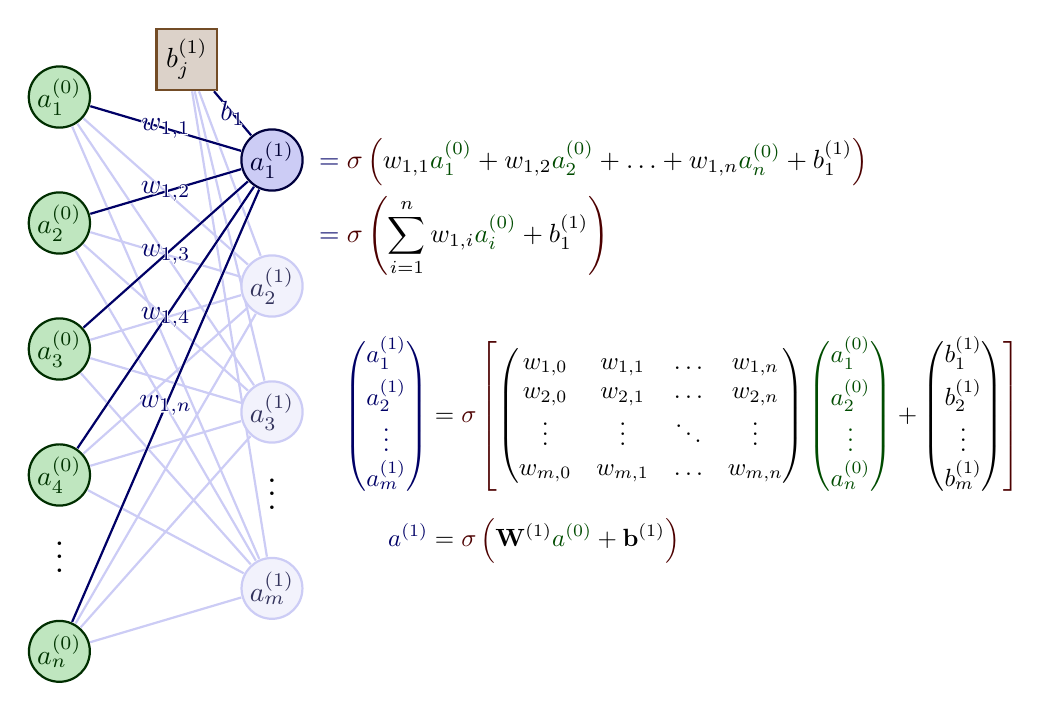
\begin{tikzpicture}[x=2.7cm,y=1.6cm]
  \message{^^JNeural network activation}
  \def\NI{5} % number of nodes in input layers
  \def\NO{4} % number of nodes in output layers
  \def\yshift{0.4} % shift last node for dots
  
  % INPUT LAYER
  \foreach \i [evaluate={\c=int(\i==\NI); \y=\NI/2-\i-\c*\yshift; \index=(\i<\NI?int(\i):"n");}]
              in {1,...,\NI}{ % loop over nodes
    \node[node in,outer sep=0.6] (NI-\i) at (0,\y) {$a_{\index}^{(0)}$};
  }
  
 

  % OUTPUT LAYER
  \foreach \i [evaluate={\c=int(\i==\NO); \y=\NO/2-\i-\c*\yshift; \index=(\i<\NO?int(\i):"m");}]
    in {\NO,...,1}{ % loop over nodes
    \ifnum\i=1 % high-lighted node
      \node[node hidden]
        (NO-\i) at (1,\y) {$a_{\index}^{(1)}$};
      \foreach \j [evaluate={\index=(\j<\NI?int(\j):"n");}] in {1,...,\NI}{ % loop over nodes in previous layer
        \draw[connect,white,line width=1.2] (NI-\j) -- (NO-\i);
        \draw[connect] (NI-\j) -- (NO-\i)
          node[pos=0.50] {\contour{white}{$w_{1,\index}$}};
      }
    \else % other light-colored nodes
      \node[node,blue!20!black!80,draw=myblue!20,fill=myblue!5]
        (NO-\i) at (1,\y) {$a_{\index}^{(1)}$};
      \foreach \j in {1,...,\NI}{ % loop over nodes in previous layer
        %\draw[connect,white,line width=1.2] (NI-\j) -- (NO-\i);
        \draw[connect,myblue!20] (NI-\j) -- (NO-\i);
      }
    \fi
  }

  %\node[node] (b1) at (0.8, 1.5) {$b_1$};
  \node[bias] (B) at (0.6,1.8) {$b_j^{(1)}$}; 
  \draw[connect,white,line width=1.2] (B) -- (NO-1);
  \draw[connect] (B) -- (NO-1) node[pos=0.50] {\contour{white}{$b_1$}};

  % INPUT LAYER
  \foreach \i in {2,...,\NO}{ % loop over nodes
    \draw[connect, myblue!20, on layer=back] (B) -- (NO-\i);
    }


  % DOTS
  \path (NI-\NI) --++ (0,1+\yshift) node[midway,scale=1.2] {$\vdots$};
  \path (NO-\NO) --++ (0,1+\yshift) node[midway,scale=1.2] {$\vdots$};
  
  % EQUATIONS
  \def\agr#1{{\color{mydarkgreen}a_{#1}^{(0)}}}
  \node[below=17,right=11,mydarkblue,scale=0.95] at (NO-1)
    {$\begin{aligned} %\underset{\text{bias}}{b_1}
       &= \color{mydarkred}\sigma\left( \color{black}
            w_{1,1}\agr{1} + w_{1,2}\agr{2} + \ldots + w_{1,n}\agr{n} + b_1^{(1)}
          \color{mydarkred}\right)\\
       &= \color{mydarkred}\sigma\left( \color{black}
            \sum_{i=1}^{n} w_{1,i}\agr{i} + b_1^{(1)}
           \color{mydarkred}\right)
     \end{aligned}$};
  \node[right,scale=0.9] at (1.3,-1.3)
    {$\begin{aligned}
      {\color{mydarkblue}
      \begin{pmatrix}
        a_{1}^{(1)} \\[0.3em]
        a_{2}^{(1)} \\
        \vdots \\
        a_{m}^{(1)}
      \end{pmatrix}}
      &=
      \color{mydarkred}\sigma\left[ \color{black}
      \begin{pmatrix}
        w_{1,0} & w_{1,1} & \ldots & w_{1,n} \\
        w_{2,0} & w_{2,1} & \ldots & w_{2,n} \\
        \vdots  & \vdots  & \ddots & \vdots  \\
        w_{m,0} & w_{m,1} & \ldots & w_{m,n}
      \end{pmatrix}
      {\color{mydarkgreen}
      \begin{pmatrix}
        a_{1}^{(0)} \\[0.3em]
        a_{2}^{(0)} \\
        \vdots \\
        a_{n}^{(0)}
      \end{pmatrix}}
      +
      \begin{pmatrix}
        b_{1}^{(1)} \\[0.3em]
        b_{2}^{(1)} \\
        \vdots \\
        b_{m}^{(1)}
      \end{pmatrix}
      \color{mydarkred}\right]\\[0.5em]
      {\color{mydarkblue}a^{(1)}}
      &= \color{mydarkred}\sigma\left( \color{black}
           \mathbf{W}^{(1)} {\color{mydarkgreen}a^{(0)}}+\mathbf{b}^{(1)}
         \color{mydarkred}\right)
         %\color{black},\quad \mathbf{W}^{(0)} \in \mathbb{R}^{m\times n}
    \end{aligned}$};
  
\end{tikzpicture}
    \caption{This is an illustration of how information is passed through and processed in a neural network.
Generated using TikZ \cite{tikz}}
    \label{fig:nnfig}
\end{figure}




\subsection{Backpropagation}
Backpropagation\cite{backprop_original} is a fundamental algorithm in training artificial neural networks.
It calculates the gradient of the loss function with respect to all the weights and biases in the network,
allowing for updating these parameters to reduce the loss.
The algorithm is based on four key equations, which we describe in this section.\\

We define the error in the $j^\text{th}$ neuron in the $l^\text{th}$ layer by
\begin{equation}\label{eq:bp1} 
    \delta_j^l = \frac{\partial C}{\partial z_j^l} = \frac{\partial C}{\partial a_j^l} \sigma '(z_j^l)
\end{equation}

This can also be considered the partial derivative of the cost function with respect to the bias in neuron $j$ in layer $l$, as 

\begin{equation}\label{eq:bp2}
    \delta_j^l = \frac{\partial C}{\partial z_j^l} = \frac{\partial C}{\partial b_j^l} \frac{\partial b_j^l }{\partial z_j^l} = \frac{\partial C}{\partial b_j^l},
\end{equation}
where we have used the relation $\partial b_j^l / \partial z_j^l = 1$ from rearranging equation \eqref{eq:z_neuron}.
The next equation relates the error in a neuron with the errors in the neurons in the subsequent layer.
\begin{equation}\label{eq:bp3}
    \delta_j^l = \frac{\partial C}{\partial z_j^l} = \sum_k \frac{\partial C}{\partial z_k^{l+1}} \frac{\partial z_k^{l+1}}{\partial z_j^l} = \sum_k \delta_k^{l+1} \frac{\partial z_k^{l+1}}{\partial z_j^l} = \left( \sum_k \delta_k^{l+1} w_{kj}^{l+1} \right) \sigma '(z_j^l)
\end{equation}
Note that the indices on the weight $w$ are now swapped.
We may think of this equation as an error propagating backward by multiplying the error in layer $l+1$ with the transpose of the weight connecting layer $l$ with $l+1$
We derive the final equation from the partial derivative of the cost function with respect to the weight $w_{jk}^l$
\begin{equation}\label{eq:bp4}
    \frac{\partial C}{\partial w_{jk}^l} = \frac{\partial C}{\partial z_j^l} \frac{\partial z_j^l}{\partial w_{jk}^l} = \delta_j^l a_k^{l-1}
\end{equation}

Equation \eqref{eq:bp1} lets us calculate the error in the last layer, and using equation \eqref{eq:bp3}, we can propagate this error backward through the network, calculating the error for all the neurons.
We then use equations \eqref{eq:bp2} and \eqref{eq:bp4} to calculate the gradient of the cost function with respect to the weights and biases.


\subsection{Gradient Descent}
Gradient Descent (GD) is an iterative optimization algorithm used in machine learning for minimizing a differentiable function.
The goal of GD is to update the model's trainable parameters in such a way that the loss function is minimized.
In mathematical terms, we aim to find the values of the parameters $\boldsymbol{\theta}$ that minimize the objective function $\mathcal{L}(\bold{x}, \boldsymbol{\theta})$, where $\bold{x}$ represents the input data.
The loss function is typically defined as the mean squared error \eqref{eq:mse} for regression problems, so
\begin{equation}
    \mathcal{L}(\bold{x}, \boldsymbol{\theta}) = \frac{1}{N}\sum_{i=1}^N(y_i-f(\bold{x}_i, \boldsymbol{\theta}))^2,
\end{equation}
where $f(\bold{x}_i, \boldsymbol{\theta})$ is the output of the model for input data $\bold{x}_i$, and $y_i$ is the target value.

To achieve the goal, GD involves calculating the gradient of the loss function with respect to the model's trainable parameters and updating them iteratively by taking a small step in the negative direction of the gradient.
The iterative update rule can be expressed as follows:

\begin{align}
\bold{v}_t &= \eta_t \nabla_\theta \mathcal{L}(\bold{x}, \boldsymbol{\theta}), \\
\boldsymbol{\theta}_{t+1} &= \boldsymbol{\theta}_t - \bold{v}_t,
\end{align}

where $\eta$ denotes the learning rate, and $\nabla_\theta$ denotes the gradient with respect to $\boldsymbol{\theta}$.
The learning rate determines the step size of the update, and it is important to choose a suitable value to ensure convergence of the optimization.

One major limitation of GD is that it can get stuck in local minima, yielding suboptimal results.
The choice of initial parameter values $\boldsymbol{\theta}$ can also impact the final optimized model.
Moreover, computing the gradient using the entire dataset can be computationally expensive for large datasets.
To address these limitations, various modifications of GD have been proposed,
such as stochastic gradient descent (SGD) and mini-batch gradient descent (MBGD),
which compute the gradient using only a subset of the data at each iteration.
These modifications can help to accelerate the convergence and improve the scalability of GD.

\subsection{Stochastic Gradient Descent}
Stochastic Gradient Descent (SGD) is a widely used optimization algorithm in machine learning that addresses some of the limitations of Gradient Descent (GD).
Unlike GD, which computes the gradient using the entire dataset at each iteration, SGD computes the gradient using only a randomly sampled subset, called a mini-batch.
This makes SGD more efficient and less computationally expensive than GD, particularly for large datasets.
Furthermore, by randomly sampling mini-batches, SGD is more likely to escape local minima and converge to the global minimum.
The update rule for SGD can be derived similarly to that for GD, with the only difference being the replacement of the full dataset with a mini-batch.
By iteratively updating the model's parameters using mini-batches, SGD can converge faster and more robustly than GD.

However, SGD also has limitations to consider. If the learning rate is too large, the optimization may overshoot the minimum and fail to converge.
On the other hand, if the learning rate is too small, the optimization may converge very slowly.
In addition, if there are areas in the function space with small gradients, the optimization may stagnate and fail to converge.
To address these limitations, various modifications of SGD have been proposed, such as adaptive learning rate methods like Adagrad and RMSprop,
which adjusts the learning rate dynamically based on the history of the gradients.
These modifications can improve the stability and convergence speed of SGD.


\subsection{Momentum GPT}

In practice, SGD is mostly used with momentum.
Momentum serves as a memory of previous momenta and can improve the convergence speed of SGD, particularly in areas of the function space with low gradients, such as local minima.

The update rule for momentum can be expressed as follows:
\begin{align}
\bold{v}_t &= \gamma \bold{v}_{t-1} + \eta_t \nabla_\theta \mathcal{L}(\bold{x}, \boldsymbol{\theta}) \\
\boldsymbol{\theta}_{t+1} &= \boldsymbol{\theta}_t - \bold{v}_t,
\end{align}
where $\gamma$ is the momentum parameter with $0 \leq \gamma \leq 1$.
The momentum term considers the update of the previous step, in addition to the gradients at the current step.
By incorporating previous momenta, momentum can smooth out variations in the optimization trajectory and accelerate convergence towards the minimum.

Momentum is particularly useful when the gradient direction is consistent across many iterations, as it allows the optimization to maintain a higher velocity in the same direction.
In contrast, in areas of high variance or noisy gradients, momentum may cause overshooting and slow down convergence.
To address this, adaptive momentum methods like Adam have been proposed, which adjust the momentum parameter dynamically based on the history of the gradients.
These methods can improve the convergence speed and stability of momentum-based optimization algorithms.


\subsection{Adam GPT}
Adam is an optimization algorithm that combines the benefits of both SGD with momentum and adaptive learning rate methods.
It uses a running average of the first and second moments of the gradient to compute per-parameter adaptive learning rates.
Adam updates the parameters iteratively as follows:

\begin{align}
\bold{g}_t &= \nabla_\theta \mathcal{L}(\bold{x}, \boldsymbol{\theta}) \\
\bold{m}_t &= \beta_1 \bold{m}{t-1} + (1-\beta_1) \bold{g}_t \\
\bold{s}_t &= \beta_2 \bold{s}{t-1} + (1-\beta_2) \bold{g}_t^2\\
\hat{\bold{m}}_t &= \frac{\bold{m}_t}{1 - (\beta_1)^t} \\
\hat{\bold{s}}_t &= \frac{\bold{s}_t}{1 - (\beta_2)^t} \\
\boldsymbol{\theta}_{t+1} &= \boldsymbol{\theta}_t - \eta_t \frac{\hat{\bold{m}}_t}{\sqrt{\hat{s}_t} + \epsilon},
\end{align}

where $\bold{g}_t$ denotes the gradient at time step $t$, $\bold{m}_t$ and $\bold{s}_t$ are the first and second moment estimates, respectively.
$\beta_1$ and $\beta_2$ control the decay rate of the first and second moments, respectively.
$\eta_t$ is the learning rate, and $\epsilon$ is a regularization constant to prevent division by zero.

Adam has several advantages over other optimization algorithms, including its ability to adaptively compute per-parameter learning rates and the robustness of its estimates to noise in the gradient.
The adaptive learning rates can help speed up convergence and lead to better performance.
Furthermore, the memory of previous first and second-order gradient estimates enables the algorithm to be more robust to noise and outliers in the data.
As a result, Adam is widely used and has become the de facto standard optimization algorithm in deep learning.


\subsection{Activation functions}
Activation functions play a crucial role in training a neural network by allowing it to learn non-linear relationships between inputs and outputs.
Different activation functions have varying properties; we will discuss some of the most common ones in this section.
Properties like non-linearity, differentiability, monotonicity, smoothness, and zero-centering are important for activation functions.
Non-linearity enables the model to capture complex relationships, differentiability is necessary for calculating the derivative of the loss function with respect to the trainable weights, monotonicity helps ensure stability in activation outputs, smoothness stabilizes gradients during training, and zero-centering balances the activation distribution within the model.

\begin{itemize}
    \item Non-linearity enables the model to capture complex relationships
    \item Differentiability is necessary for calculating the derivative of the loss function with respect to the trainable weights
    \item Monotonicity helps ensure stability in activation outputs, smoothness stabilizes gradients during training
    \item Smoothness: A smooth activation function helps stabilize the gradients and training.
    \item Zero-centering balances the activation distribution within the model.
\end{itemize}

\paragraph{Tanh}
Tanh, the hyperbolic tangent function is given by
\begin{equation}\label{eq:tanh}
    Tanh(x) = \frac{e^x+e^{-x}}{e^x-e^{-x}}
\end{equation}

\paragraph{ReLU}
The Rectified Linear Unit (ReLU) activation function pushes all negative values to zero while leaving positive values unchanged,
which introduces non-linearity while solving the vanishing gradients problem by having a gradient of either 0 or 1 for negative and positive values, respectively.
\begin{equation}\label{eq:relu}
    ReLU(x) = \begin{cases} x & \mbox{if } x > 0 \\ \mbox{0,} & \mbox{otherwise} \end{cases}
\end{equation}

\paragraph{GeLU}
The Gaussian Error Linear Unit (GeLU) is a smooth approximation of the ReLU function, given by
\begin{equation}
    GeLU(x) = x \Phi (x),
\end{equation}
where $\Phi(x)$ is the standard Gaussian cumulative distribution function.

GeLU can be approximated with
\begin{equation}
    GeLU(x) \approx 0.5x \left( 1+\tanh\left[\sqrt{2/\pi}(x+0.044715x^3)\right] \right),
\end{equation}
which is faster to compute than the original definition but can result in worse performance.
For computational efficiency, we used this approximation.


\section{Model Explainability}
In the context of machine learning, SHAP \cite{SHAP} and SAGE \cite{SAGE} apply the same idea to determine the contribution of each feature to a prediction.
SHAP provides a local explanation by computing the contribution of each feature to the prediction of a single data point.
On the other hand, SAGE provides a global explanation by computing each feature's contribution to the model's overall prediction performance.
These methods allow us to understand the relationship between the features and the prediction, particularly useful when the model is too complex to interpret.
Additionally, they provide a way to validate the model's fairness and bias.
By understanding which features contribute the most to a prediction, one can determine if the model is fair or biased and if the prediction is trustworthy.\\

Both SHAP and SAGE methods are based on Shapley values \cite{shapley_value_1953}, a concept in game theory introduced by Lloyd Shapley in 1951.
Shapley values determine each player's contribution to a group's surplus or overall value.
The explanation below of Shapley values, SHAP, and SAGE is inspired by a blog post by Ian Covert \cite{covert_shap_sage}.\\

The Shapley value for a player $i$ in a cooperative game with $d$ players is

\begin{equation}
    \phi_i(w) = \frac{1}{d} \sum_{S \subseteq D \backslash \{ i \} } \binom{d-1}{|S|}^{-1} \left[ w(S\cup \{ i \} ) - w(S) \right]
\end{equation}

where $D$ is the set of all players, $S$ is a coalition of players, $w(S)$ is the value of the coalition $S$, and $|S|$ is the number of players in the coalition.
This formula satisfies four important conditions:
\begin{itemize}
    \item Efficiency: The sum of all Shapley values is equal to the group's total value.
    \item Symmetry: If two players $i$ and $j$ have the same impact on all coalitions with $w(S \cup \{i\}) = w(S \cup \{j\})$ for all $S$, they should have the same Shapley value $\phi_i(w) = \phi_j(w)$.
    \item Dummy: A player $i$ that makes no contribution to the group with $w(S \cup \{i\}) = w(S)$, should receive a value of zero, or $\phi_i(w)=0$.
    \item Linearity: A player's value is proportional to their contribution to the group.
If player $i$ contributes twice as much as player $j$ to the group's overall worth, then player $i$ should have twice the Shapley value.
\end{itemize}

\subsection{SHAP}
Shapley values explain how each feature $(x^1, \dots, x^d)$ in a model $f$ contributes to the deviation from the mean prediction $\mathbb{E}[f(x)]$ of the dataset for a single prediction.
It assigns a value $\phi_1, \dots, \phi_d$ to each feature that quantifies the feature's influence on the prediction $f(x)$.
SHAP (Shapley Additive Explanations) computes approximate Shapley values for machine learning models.\\

We define a cooperative game $v_{f,x}$ to represent a prediction given the features $x^S$, as
\begin{equation}
    v_{f,x}(S) = \mathbb{E} \left[ f(X) | X^S = x^S \right],
\end{equation}

where $x^S$ are known, and the remaining features are treated as random variable $X^{\Bar{S}}$ (where $\Bar{S} = D \backslash S$).
This is the mean prediction $f(X)$ when the unknown values follow the conditional distribution $X^{\Bar{S}} | X^S = x^S$.\\

Using a subset of features from the prediction while sampling the rest from the dataset reduces the chance of improbable samples.
Given this convention for making predictions, we can apply the Shapley value to define each feature's contribution to the prediction $f(X)$ using Shapley values $\phi_i(v_{f,x})$.
A Shapley value of $\phi_i(v_{f,x}) > 0$ indicates that feature $i$ contributes to an increase in prediction $f(X)$.
A negative Shapley value $\phi_i(v_{f,x}) < 0$ indicates the opposite, that the feature contributes to a decrease in $f(X)$.
Uninformative features will have small values $\phi_i(v_{f,x}) \approx 0$.

\subsection{SAGE}
SAGE (Shapley Additive Global Importance) explains how every feature contributes to the model's overall performance, and it relates to SHAP in a simple way.
For a given feature, the global feature importance is the average SHAP value (for that feature) across all samples in the dataset.
This is, however, different from how it is calculated in practice.
A paper by Ian Covert et al.
\cite{sage_paper} on global feature importance proposes an algorithm that aims directly at a global feature explanation, unlike the SHAP values, which makes
it faster.
This is the algorithm used for approximating the SAGE values for the features in the thesis.

\section{Mutual Information}
Mutual information is a fundamental measure of the statistical dependence between two random variables,
providing a way to quantify the amount of information one variable conveys about the other.
For a pair of discrete random variables $X$ and $Y$, we have 
\begin{equation}
    I(X;Y) = \sum_{y} \sum_{x} p(x,y) \log \left( \frac{p(x,y)}{p(x)p(y)} \right),
\end{equation}
where $p(x,y)$, $p(x)$, and $p(y)$ are the joint and marginal probabilities, respectively.
The mutual information captures linear and nonlinear relationships between variables, unlike Pearson's correlation coefficient, which can only detect linear relationships.
However, mutual information has limitations in that it relies on binning the data, which can introduce bias and limit the resolution of the information.
   
Furthermore, estimating mutual information for high-dimensional data sets can be computationally expensive.
Despite these limitations, mutual information remains a popular tool in feature selection, data visualization, and machine learning.

\chapter{Method}
In this section, I explain the data analysis, cleaning, transformation, feature engineering, and models.

\section{Cleaning pointing scan data}
\subsection{Cleaning rules}
The pointing scan data is noisy, and contains a lot of outliers.
In order to make the data more suitable for machine learning, we need to clean the data.
Below is a list of some criteria we use to filter out scans.
\begin{itemize}
    \item Scans using the HOLO transmitter.
    These scans are aiming at a radio tower, and is therefore not realistic data to train the ML model with.
    \item Scans using ZEUS2.
    These are highly experimental pointing scans and unreliable.
    \item Scans using CHAMP690, as there are very few scans using this instrument.
    \item Scans in January and February.
    There are not many scans in this time period, and the few we have involve a lot of testing.
    \item Scans that are tracking tests.
\end{itemize}   
\textcolor{red}{Find the proportion of scans that are removed from the above list.}
After this filtering, there are x out of 8862 scans left.
        
\subsection{Pointing scan classifier}
\subsubsection{Method}
In addition to the cleaning rules, we have to remove the ouright bad pointing scans (like \ref{subfig:bad_continuous} \ref{subfig:bad_line}, \ref{subfig:bad_line}).
This is done by training a classifier predict whether a scan is good or bad.
We used an XGBoost classifier with 13 features as inputs, all of which are present in the pointing scan figures (\ref{fig:line_pointings} and \ref{fig:continueous_pointings}).
The first 12 features are the amplitudes, FWHMs and pointing offsets, along with the uncertainties of these values.
The last feature is the beamsize of the telescope for the given observing frequency.\\

We had to label a training set by manually looking at pointing scans.
The size of the training set was $369$ with $270$ good and $99$ bad scans.
We did a hyperparameter search for the max depth between $1$ and $5$, number of estimators between $1$ and $80$, 
and used the \textit{scale\_pos\_weight} to consider the unbalanced classes.
The value for this parameter is the ratio of negative to positive classes.
$80\%$ of the data was used for training, and the rest for testing, which corresponds to $295$ and $74$ samples for training and testing respectively.


\begin{itemize}
    \item What hyperparameters were tuned, and what are the values.
    \item Show why it is hard to clean by only noise
    \item labeling trainig set manually, size and proportion of pos neg
    \item can choose how strict we want to be on the cleanliness
    \item precicion recall curve or mAP curve?onda
\end{itemize}

\subsubsection{Results}
The XGBoost classifier performed well a $97\%$ overall accuracy on the test set.
Figure \ref{fig:pointing_scan_clf} shows the precicion-recall curve on the left and the average precision curve on the right.
From the precision-recall curve it is clear that we can achieve a close to $100\%$ precision while still having a high recall.
This is ideal, as we want the training data for the pointing model to be as clean as possible.
We can select a large threshold, such that very few bad scans end up in the training data.
The average precicion curve shows an optimal threshold for maximizing the precision, which is about $80\%$.

\begin{figure}[H]
    \centering
    \begin{subfigure}[t]{0.49\textwidth}
        \centering
        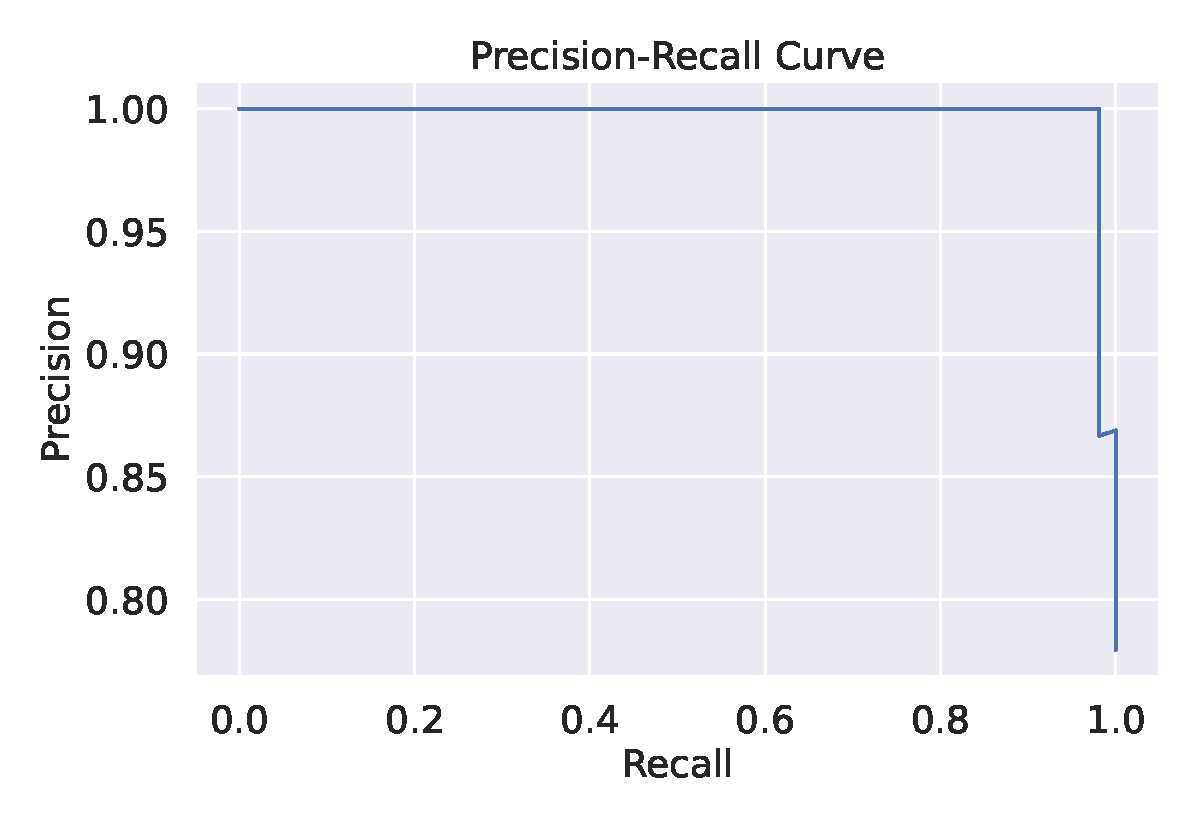
\includegraphics[width=1\textwidth]{Clf/precision_recall_curve_both.pdf}
        \caption{Precision-recall curve on test set.}
        \label{subfig:pr_curve}
    \end{subfigure}
    \begin{subfigure}[t]{0.49\textwidth}
       \centering
       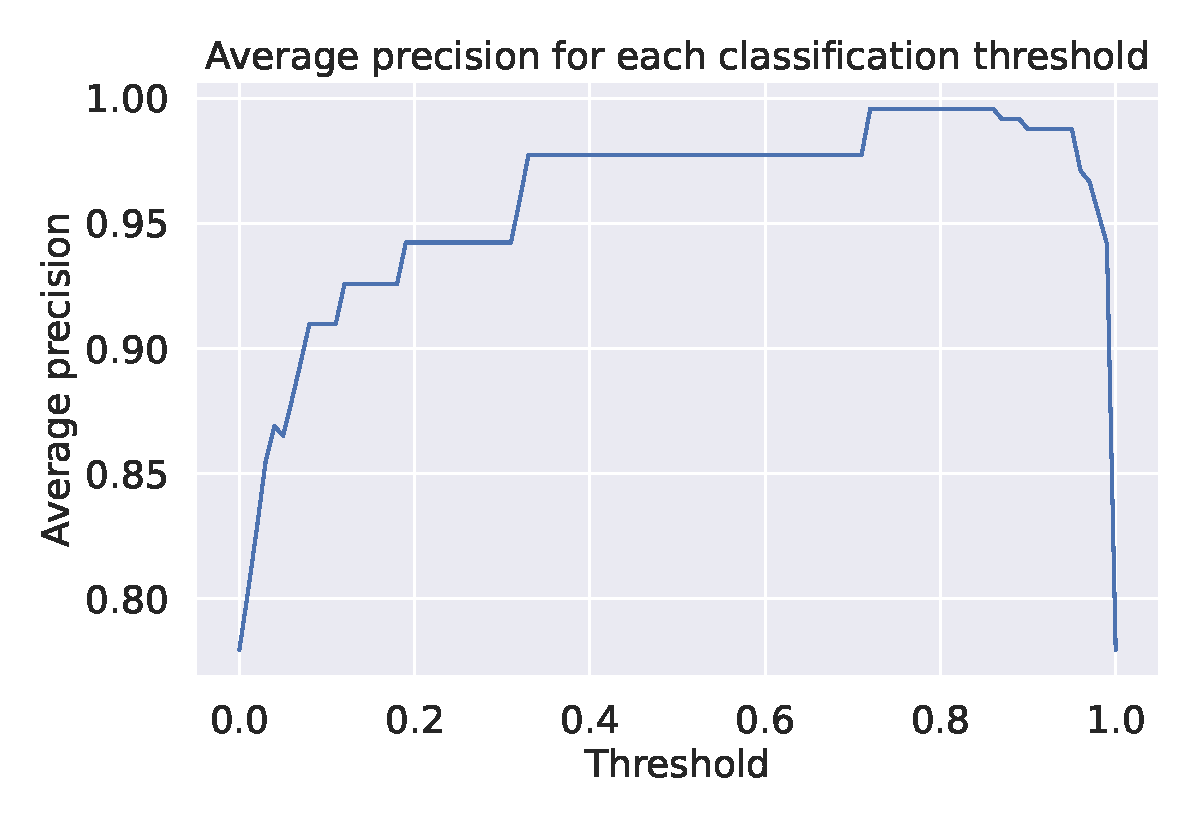
\includegraphics[width=1\textwidth]{Clf/mAP_curve_both.pdf}
       \caption{Average precision for different classification threshold.}
       \label{subfig:map_curve}
    \end{subfigure}
     \caption{Precision-recall and average precision curve for the XGBoost classifier when classifying good and bad pointing scans in the test set.}
     \label{fig:pointing_scan_clf}
\end{figure}

% \\~\\
% \begin{subfigure}[t]{0.49\textwidth}
%     \centering
%     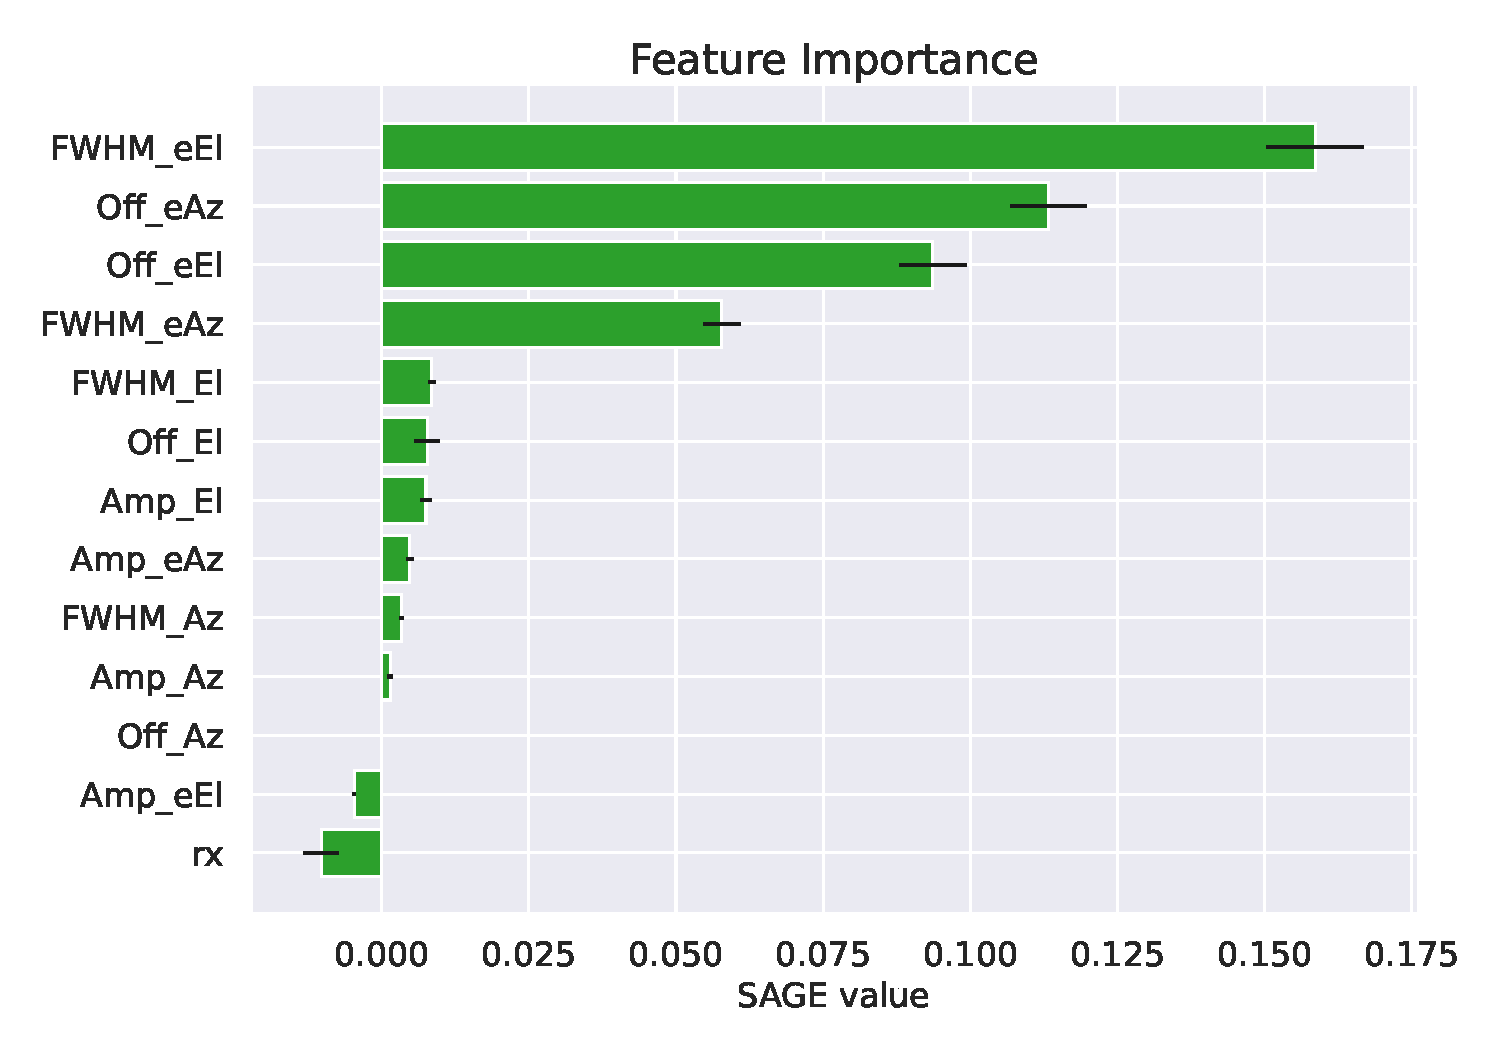
\includegraphics[width=1\textwidth]{Clf/Sage_xgb_clf_rx.pdf}
%     \caption{Average precision for different classification threshold.}
%     \label{subfig:xgb_clf_sage}
% \end{subfigure}
% \begin{figure}[H]
%     \centering
%     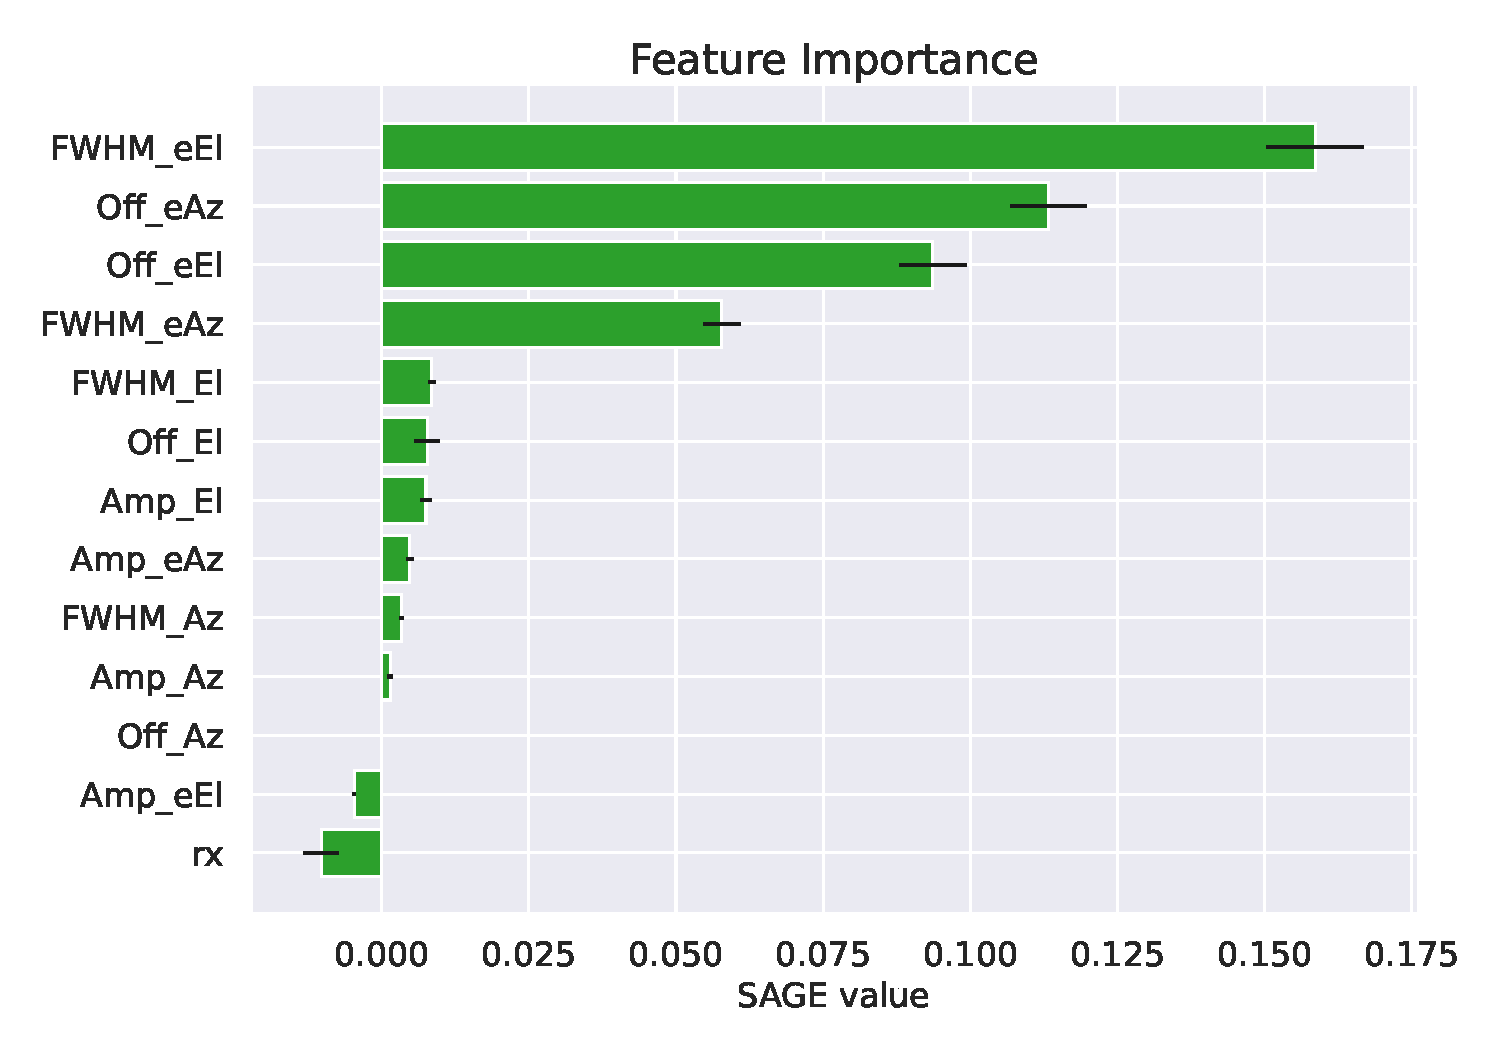
\includegraphics[width=0.98\textwidth]{Clf/Sage_xgb_clf_rx.pdf}
%     \caption{SAGE values for the XGB classifier.}
%     \label{fig:xgb_clf_sage}
% \end{figure}

\section{Scan duration analysis}
As mentioned in the database section, the timestamps of the scans is not the accurate start time of a scan.
The tiltmeter dump files with the flag indicating whether the telescope is idle, preparing to observe, or observing,
is the only data we have on when the telescope is actually performing a pointing scan.
Therefore, we need to combine the timestamp of the pointing scan with the flag in the dump files to analyse the duration of scans.

\subsection{Method}
First, we convert the different scan flags to numbers.
\textit{IDLE} and \textit{PREPARING} is the set $0$, and \textit{OBSERVING} is set to $1$.
Then we can subtract the previous rows from all rows, which will result in a value of $1$ when the scan starts, and $-1$ when it ends.
Table \ref{tab:scan_flag_difference} shows an example of the resulting table.


\begin{table}[H]
    \centering
    \begin{tabular}{cccc}
        \toprule
        Time & Flag & Flag Integer & $\Delta$ \\
        \midrule
        11:21:21 & IDLE & $0$ & $0$ \\
        11:21:22 & PREPARING & $0$ & $0$ \\
        11:21:23 & OBSERVING & $1$ & $1$ \\
        11:21:24 & OBSERVING & $1$ & $0$ \\
        11:21:25 & OBSERVING & $1$ & $0$ \\
        11:21:26 & IDLE & $0$ & $-1$ \\
        \bottomrule
    \end{tabular}
    \caption{This table shows the tiltmeter dump file containing the telescope state flag,
            and how we find the start ($\Delta = 1$) and end ($\Delta = -1$) of a scan.}
    \label{tab:scan_flag_difference}
\end{table}

By analyzing these tables for all the scans we had tiltmeter dumps for,
we see that the first \textit{OBSERVING} flag present after a scan is about $53$ \textcolor{red}{Add accurate mean and standard deviation} seconds after the scan timestamp for the vast majority of the scans.
This is shown in the right plot in figure \ref{fig:scan_times_box}, which strongly indicates that this is the starting point of a pointing scan.
In the same plot, we also see that this is fairly constant for the different instruments.
The right plot of figure \ref{fig:scan_times_date} show the time difference in seconds between the first observing flag after a scan timestamp throughout the year.
From the plot, we may conclude that this stays constant over time.\\

Now that we have found the start of a pointing scan, we look at the durations of the scans.

The left plots in figure \ref{fig:scan_times_date} and \ref{fig:scan_times_box} show the duration of the pointing scans for different instruments.
From this figure, it is clear that the duration of a pointing scan varies a lot.
This is problematic because of the fact that we only have these tiltmeter dump files for $2862/8381\approx 34\%$ of the pointing scans.


\begin{figure}[H]
    \centering
    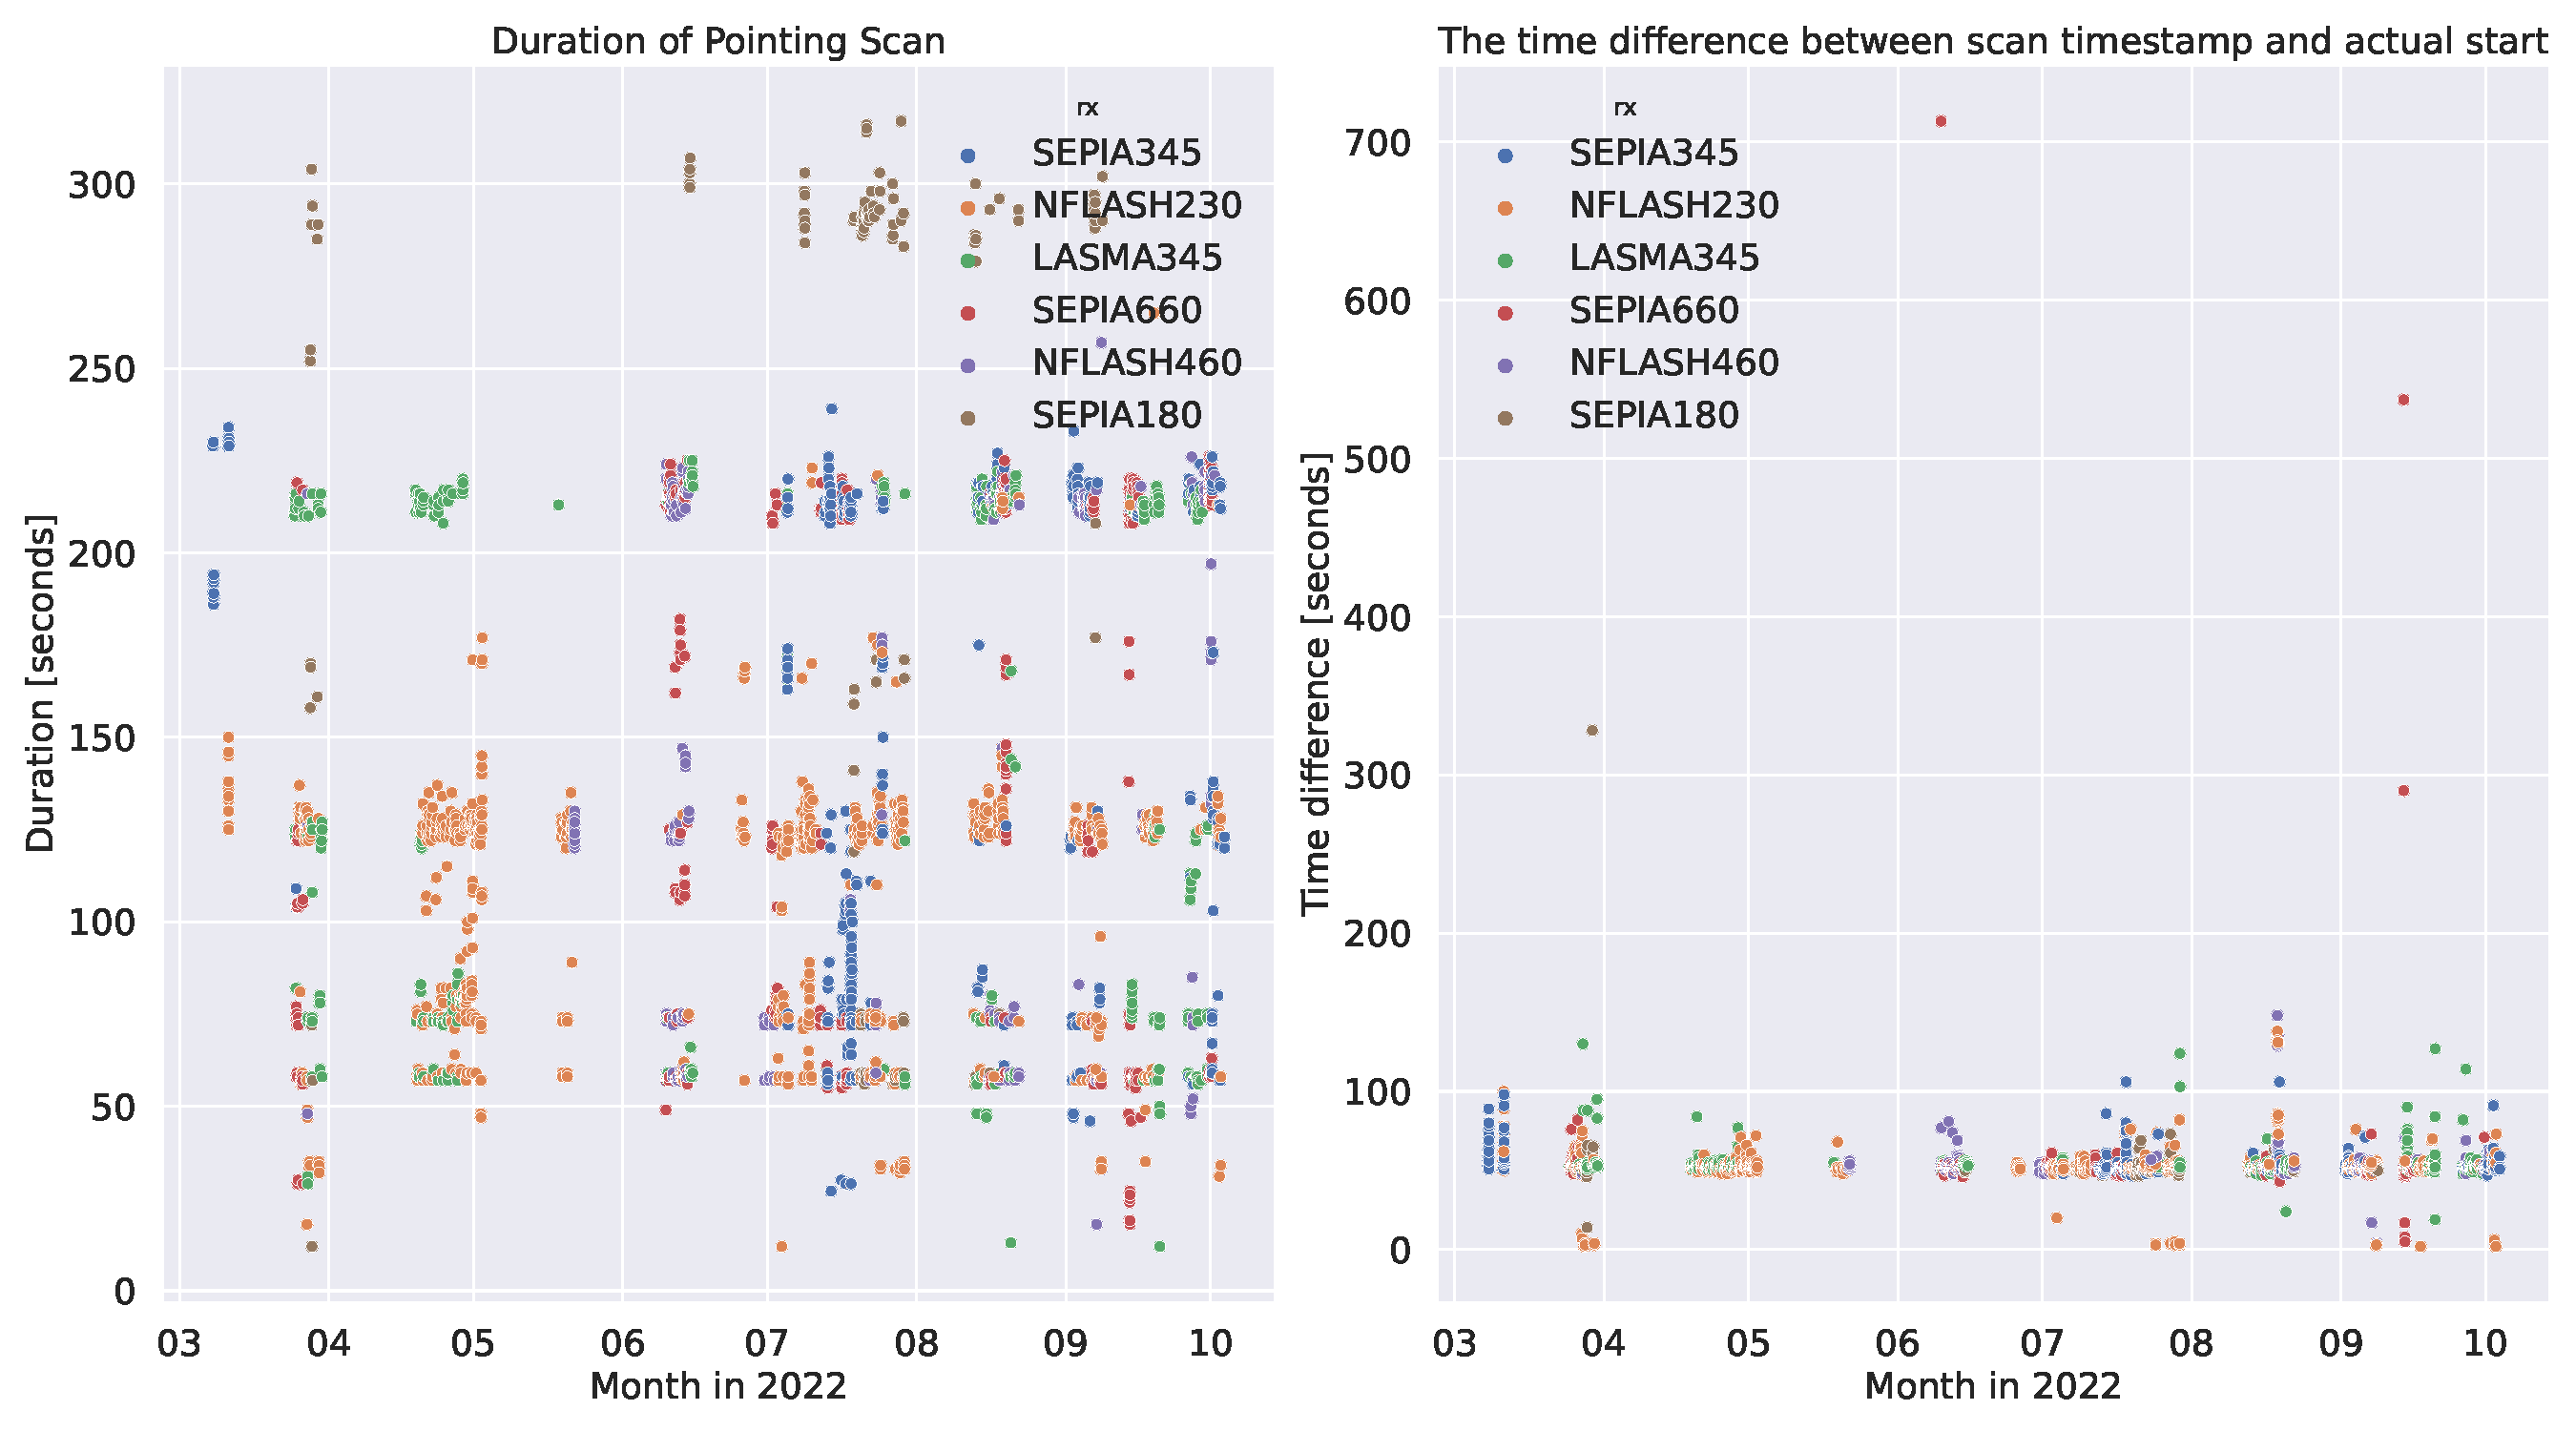
\includegraphics[width=1.1\textwidth]{Tiltmeter plots/scan_duration_distribution_date.pdf}
    \caption{Scatter plot of the duration of scans, and the time difference between the timestamp of a scan and the actual start of it.}
    \label{fig:scan_times_date}
\end{figure}

\begin{figure}[H]
    \centering
    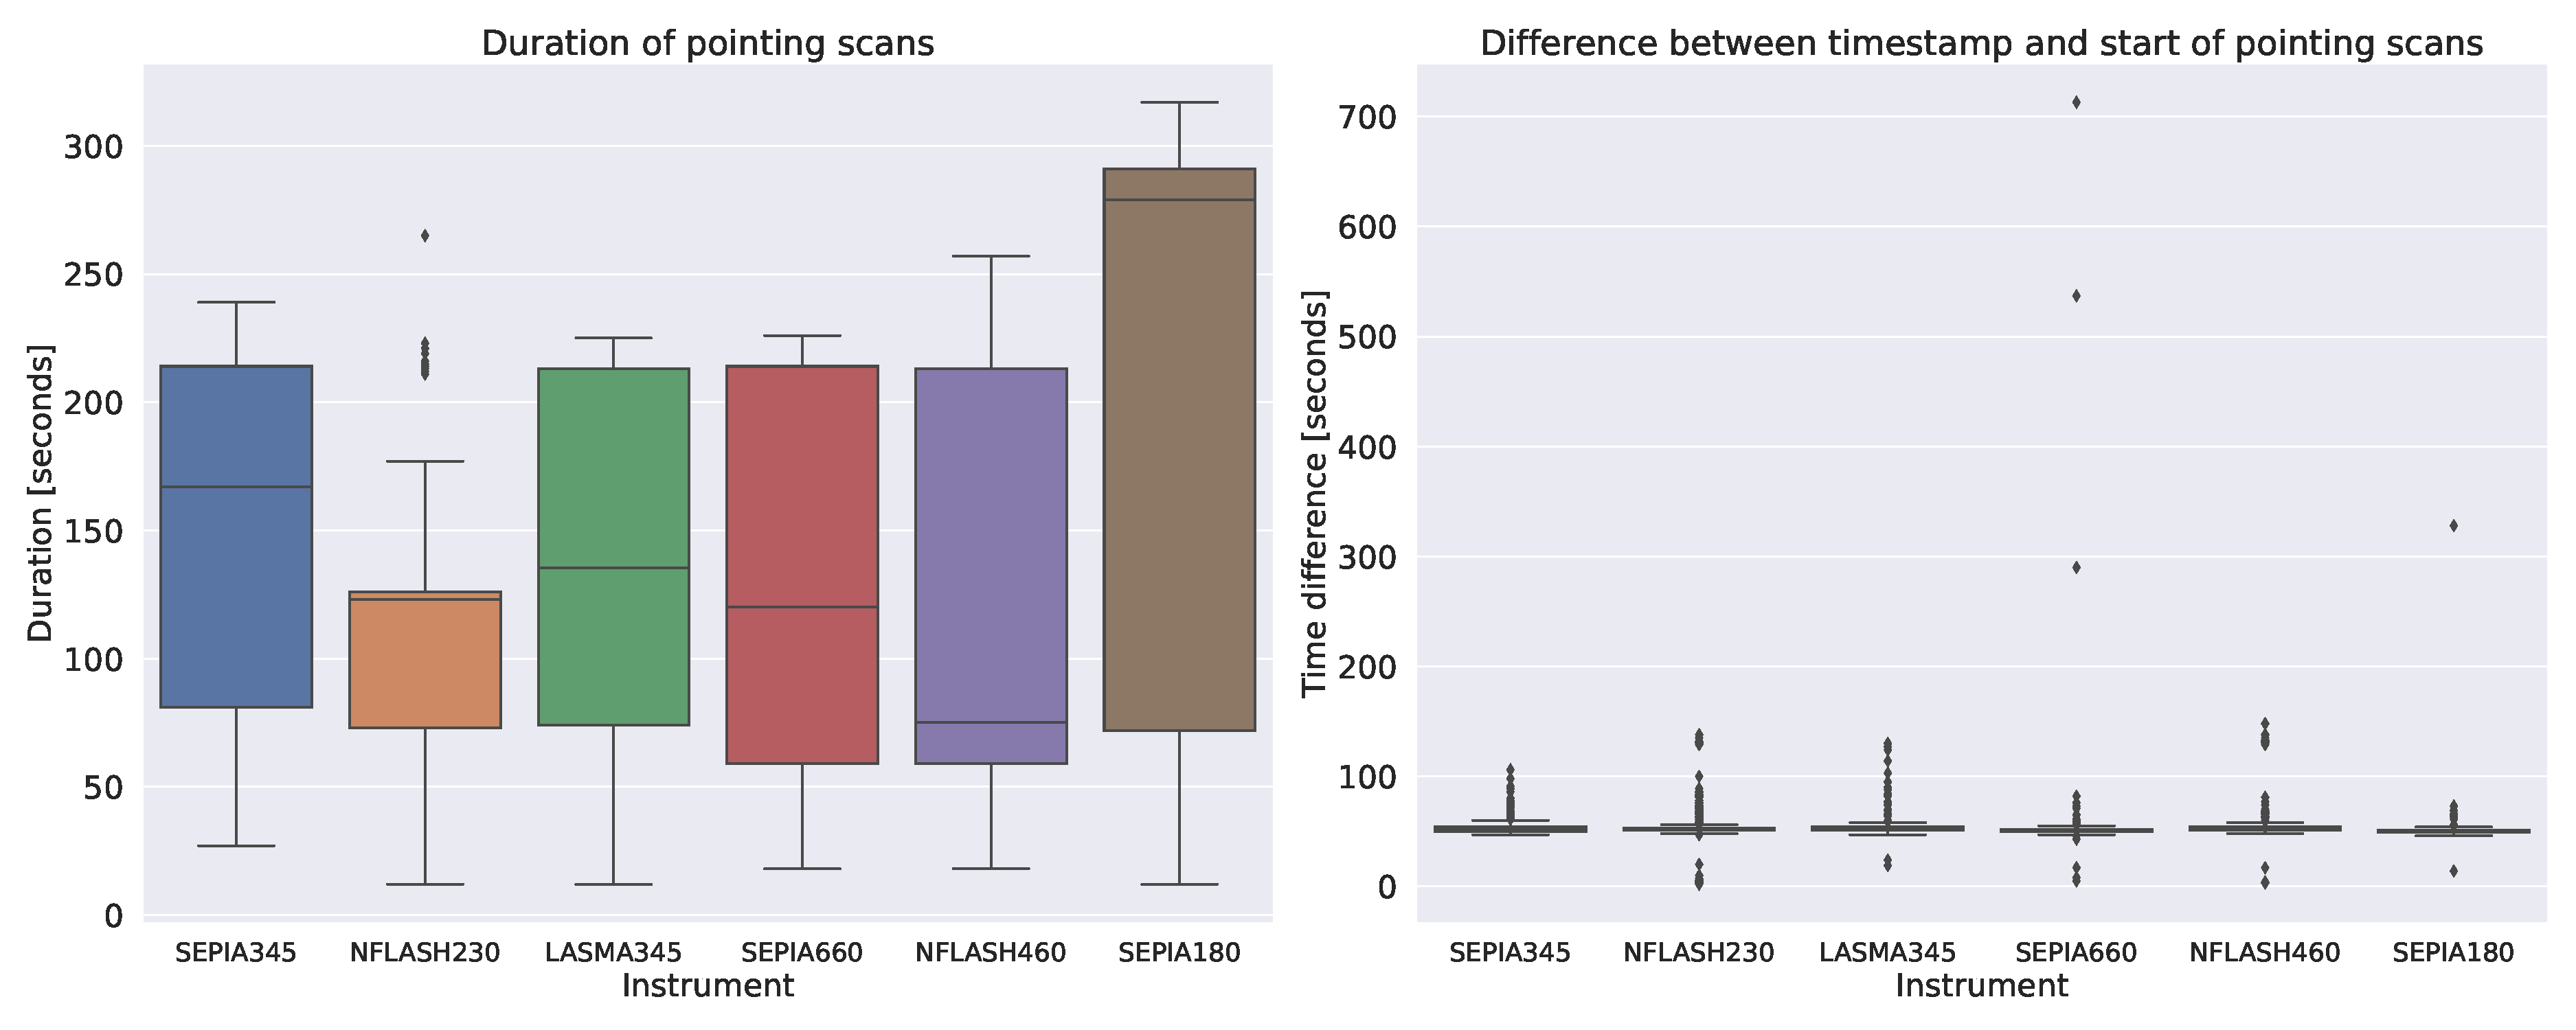
\includegraphics[width=1.1\textwidth]{Tiltmeter plots/scan_duration_distribution_rx.pdf}
    \caption{Box plot of the duration of scans, and the time difference between the timestamp of a scan and the actual start of it.}
    \label{fig:scan_times_box}
\end{figure}


\subsection{Algorithm}
Following is the algorithm used to obtain the start and end of pointing scans using the scan timestamp and the observing flag from tiltmeter dumps.

\begin{algorithm}[H]
    \caption{Find start and end of pointing scan}
    \label{alg:scan_times}
    \begin{algorithmic}
        \Require{\\
        \begin{itemize}
            \item Pointing scan timestamps $D=\{D_1,\dots,D_n\}$
            \item Timestamps $T=\{T_1,\dots,T_m\}$ and scan flag $F=\{F_1,\dots,F_m\}$
        \end{itemize}}
        \Ensure{Start and end of pointing scans $S=\{S_i,\dots,S_n\}$ and $E=\{E_i,\dots,E_n\}$}
        \For{$i=1,\dots,m$}
            \If {$F_i=OBSERVING$}
                \State {$F_i = 1$}
            \Else
                \State {$F_i = 0$}
            \EndIf
        \EndFor
        \\
        \For{$i=1,\dots,n$}
            \State {$\hat{T} = \{T_j, \text{  if  } T_j > D_i\}_j^m$}
            \State {$\hat{F} = \{F_j, \text{  if  } T_j > D_i\}_j^m$}
            \ForAll {$t_i,f_i \text{ in } \hat{T},\hat{F}$}
                \State {$\Delta = f_i-f_{i-1}$}
                \If {$\Delta = 1$}
                    \State {$S_i = t_i$}
                \EndIf
                \If {$\Delta = -1$}
                    \State {$E_i = t_i$}
                    \State {Continue}
                \EndIf
            \EndFor
        \EndFor
    \end{algorithmic}
\end{algorithm} 


\section{Feature Engineering}
\subsection{Different calculations}
There are two main types of features engineered for this project.
Features that represent the system during a pointing scan, and features that represent the changes since the last correction. 
The idea behind this is simple. The correction used during a pointing scan represents the ideal correction for the system during the previous pointing scan
As there are a lot of factors and complex relationships, and we don't have large amounts of training data, it might be easier for the model to learn 
how these changes affect the pointing rather than learning all the relationships.

\paragraph{Median values}
The median value of variables during a pointing scan is the most used feature.
Table \textcolor{red}{ref table with list of variables with median value} shows the list of variables for which we use the median values during a pointing scan.
\paragraph{Sum of all change}
To capture systematic error in pointing due to the telescope moving back and forth in azimuth and elevation,
we sum over the positive and negative changes in these variables.

Given the time of the last pointing correction $t_1$ and the start of a pointing scan $t_2$, the sum over the positive changes in a variable $x_i$ is given by
\begin{equation}\label{eq:positive_int}
    \sum_{i=t_1+1}^{t_2} \max(0, x_i-x_{i-1})
\end{equation}

Similarly, the sum of negative changes in a variable is
\begin{equation}\label{eq:negative_int}
    \sum_{i=t_1+1}^{t_2} \min(0, x_i-x_{i-1})
\end{equation}

These features are made for azimuth and elevation.

\paragraph{Change since last correction}
This feature is self-explanatory and is just the change in a variable since the pointing was corrected.
\begin{equation}
    \Delta x = x_{t_2} - x_{t_1}
\end{equation}

In order to make this feature more robust against noisy data,
we instead look at the change in the median for a time interval around the last correction $t_1$ and the start of a pointing scan $t_2$

\begin{equation}
    \Delta x = \textit{median}(x_{t_2}, x_{t_2 - 1}, \dots, x_{t_2- p}) - \textit{median}(x_{t_1}, x_{t_1 + 1}, \dots, x_{t_1 + p}),
\end{equation}
where $p$ is the number of data points needed to cover a period of $P$ minutes, given by $p = P \cdot frequency$. The unit of frequency is data points per minute, found in table \textcolor{red}{fix data freq ref}.

\paragraph{Max change in time interval}
In case the speed of the temperature change affects the deformation of the telescope's structure, we find the maximum temperature change in a given time interval since the last pointing correction.

\begin{equation}
    \max (x_{t_1+p} - x_{t_1}, x_{t_1+p} - x_{t_1}, \dots, x_{t_2} - x_{t_2-p}),
\end{equation}


\paragraph{Position of the sun}
Observers at the telescope report that the sun is affecting the pointing.
It is most drastically affected when the sun sets or rises, likely due to rapid change in temperature which leads to deformation in the telescope structure.
It is also thought that the position of the sun could play a role, and perhaps be modelled too.
For instance, if the sun is shining on the left side of the telescope, it will affect the pointing differently than if it was on the right side.
Obtaining the position of the sun for the location of the telescope is done using the python module PyEphem \cite{ephem}.

Using the azimuth angle of the sun and the telescope, we can calculate the position of the sun with respect to the pointing with
\begin{equation}\label{eq:sun_az_diff}
    \Delta \textit{Az}_\odot = \textit{Az}_{\textit{t}} - \textit{Az}_\odot
\end{equation}
This will result in values outside the $[-180^\circ,180^\circ]$. An example of this is if $Az_\odot=179^\circ$ and $Az_t = -179^\circ$.
The calculation in equation \eqref{eq:sun_az_diff} yield $-179^\circ-179^\circ=-358^\circ$,
which corresponds to the sun being $358^\circ$ to the right of the telescope, while it ideally should be $2^\circ$ to the left.
Therefore, we adjust the values accordingly
%Write equations where \Delta Az_\odot above 180 is -= 360 and under 180 is += 360
\begin{align}
    \Delta Az_\odot = Az_\odot +360^\circ, \; \text{for} \; \Delta Az_\odot < 180^\circ\\
    \Delta Az_\odot = Az_\odot -360^\circ, \; \text{for} \; \Delta Az_\odot > 180^\circ
\end{align}

Here, the interval of the difference in azimuth is fixed to the interval $(-180^\circ,180^\circ)$,
where $0^\circ$ means the telescope is pointing towards the sun in the azimuth direction.
$\Delta \textit{Az}_\odot = 90^\circ$ corresponds to the sun being direct to the left of the pointing direction. \\

Another measure tested is the total angle between the pointing and the position of the sun. This is calculated using the following formula
\begin{equation}
    \theta = \cos \textit{Az}_t \cdot \cos \textit{El}_t\cdot \cos \textit{Az}_\odot \cdot \cos \textit{El}_\odot + \sin \textit{Az}_t \cdot \cos \textit{El}_t\cdot \sin \textit{Az}_\odot \cdot \cos \textit{El}_\odot + \sin \textit{El}_t \cdot \sin \textit{El}_\odot
\end{equation}

\subsection{List of features}
\textcolor{red}{add a list of all features for different calculations here}

\section{Transformation of pointing offsets and corrections}
Table \ref{tab:offset_and_correction} shows some observed pointing offsets and the corrections applied during the pointing scan.
The pointing corrections $ca$ and $ie$ are sometimes updated according to equation \eqref{eq:ca} and \eqref{eq:ie},
as we see in the first two rows. Sometimes the corrections are not updated, like in the consecutive row. Other times, the corrections are updated, but not according to the equation \eqref{eq:ca} and \eqref{eq:ie}.
This introduces a couple of challenges for the training of a model.
\begin{itemize}
    \item $ca$ and $ie$ should represent the optimal correction using all the information we have about the current state of a system.
    If we don't update the corrections, there is some information about the system (the previously observed pointing offset) the model is not receiving.
    \item Some of the features are constructed by looking at the change in variables since the last correction.
    If the corrections are not updated, this interval is longer and the resulting features could be more prone to uncertainties and noise.
    A problem with the integration also occurs if the corrections are not updated according to the equations \eqref{eq:ca} and \eqref{eq:ie}.
    Then we don't know at what time those corrections represent the system, resulting in inaccurate features.
\end{itemize}


The following is a possible solution to these problems.
\begin{enumerate}
    \item Transform the offsets and corrections such that they represent the system at the most recent pointing scan.
    \item Use these transformed offsets as new training labels, and transformed corrections as training inputs.
\end{enumerate}

The way I do this is by assuming the corrections $ca$ and $ie$ are updated after every pointing scan.
This will change the observed pointing offsets, which again will affect the corrections during the next pointing scan.
The effects of this followed throughout the whole dataset
The following formulas 
\begin{align}
    \Tilde{ca}_i &= \Tilde{ca}_{i-1} + \Tilde{\delta}_{az,i-1}\label{eq:ca_tilde}\\
    \Tilde{ie}_i &= \Tilde{ie}_{i-1} - \Tilde{\delta}_{el,i-1\label{eq:ie_tilde}}\\
    \Tilde{\delta}_{az,i} &= \delta_{az,i} + ca_i - \Tilde{ca}_i\label{eq:off_az_tilde}\\
    \Tilde{\delta}_{el,i} &= \delta_{el,i} - ie_i + \Tilde{ie}_i\label{eq:off_el_tilde}
\end{align}
Where the "$\sim$" denotes a transformed variable.
Using these transformations,
the corrections used for training and the resulting offset are alike the ones that would be observed if the corrections were made according to the equations
\eqref{eq:ca} and \eqref{eq:ie} after every pointing scan.


\begin{table}[H]
    \centering
    \caption{Example from the dataset of the observed pointing offsets and the corrections applied during the pointing scan.}
    \label{tab:offset_and_correction}
    \begin{tabular}{ccccc}
    \toprule
    $i$ &  $\delta_{az}$ &  $\delta_{el}$ &  $ca$ & $ie$  \\
    \midrule
    1 & 1.2 & 0.1 & 2.1 &  1.7 \\
    2 &     0.0 & 0.5 & 3.3 &  1.6 \\
    3 &    -1.1 & 0.0 & 3.3 &  1.6 \\
    4 &     0.6 & 0.7 & 2.2 &  1.6 \\
    5 &     0.9 & 1.4 & 2.2 &  1.6 \\
    6 &     1.0 & 1.1 & 2.2 &  1.6 \\
    7 &    -0.9 & 1.2 & 3.1 &  0.5 \\
    8 &     0.5 & 1.5 & 2.2 & -0.7 \\
    9 &    -0.3 & 0.4 & 2.2 & -0.7 \\
    \bottomrule
    \end{tabular}
\end{table}


\begin{table}[H]
    \centering
    \caption{Table of transformed pointing offsets and corrections according to equations \eqref{eq:ca_tilde}, \eqref{eq:ie_tilde}, \eqref{eq:off_az_tilde}, and \eqref{eq:off_el_tilde}.}
    \label{tab:tranform_offsets}
\begin{tabular}{ccccc}
\toprule
$i$ & $\Tilde{\delta}_{az}$ &  $\Tilde{\delta}_{el}$ &  $\Tilde{ca}$ &  $\Tilde{ie}$ \\
\midrule
0 &       1.2 &       0.1 &       2.1 &       1.7 \\
1 &       0.0 &       0.5 &       3.3 &       1.6 \\
2 &      -1.1 &      -0.5 &       3.3 &       1.1 \\
3 &       0.7 &       0.7 &       2.2 &       1.6 \\
4 &       0.2 &       0.7 &       2.8 &       0.9 \\
5 &       0.1 &      -0.3 &       3.1 &       0.2 \\
6 &      -1.0 &       1.3 &       3.2 &       0.5 \\
7 &       0.5 &       1.4 &       2.2 &      -0.7 \\
8 &      -0.8 &      -1.1 &       2.7 &      -2.2 \\
\bottomrule
\end{tabular}
\end{table}


\section{Experiments overview}
In this section, I will provide an overview of two machine learning experiments that are pertinent to the two research questions.
The first experiment aims to investigate the effectiveness of neural networks in developing a pointing model that could potentially replace the current linear model, which is created through linear regression.
The purpose of this experiment is to explore the feasibility of a more sophisticated model in terms of pointing accuracy.
The second experiment aims to examine the effectiveness of an XGBoost model in predicting pointing scan offsets to enhance the pointing accuracy.
The primary objective of this experiment is to assess whether the proposed model can outperform the current model in terms of pointing accuracy.

\section{Experiment 1: Pointing Model using Neural Networks}
This experiment uses the raw dataset containing input coordinates, $Az_{\text{input}}$ and $El_{\text{input}}$ respectively, and corresponding true observed values $Az_{\text{observed}}$ and $El_{\text{observed}}$.

The goal is to find a model $f$ such that
\begin{equation}
    f(X) \approx (\delta_{\text{Az}}, \delta_{\text{El}}) = (Az_{\text{observed}}-Az_{\text{input}}, El_{\text{observed}}-El_{\text{input}})
\end{equation}


\subsection{Feature Selection}
Selecting the right features plays an important role in improving the accuracy of the pointing model.
This model uses two types of features: geometrical and harmonic terms that are already part of the current linear base model, and new features that are extracted from the telescope's database.
We identified relevant features by calculating Pearson's and Spearman's rank correlation for all features in relation to the offsets.
We analyzed the correlation of harmonic terms using sine and cosine functions of azimuth and elevation up to the fifth order, as well as the geometrical terms.
Then, we chose the terms that had the strongest correlation for the model and used them in all models.
For the features extracted from the database, we made a list of the ones that showed a correlation equal to or greater than 0.1.
During model training, we randomly selected a subset of 2 to 19 features from this list and used them to train the model.

\subsection{Model Architecture}
This experiment utilized four different model architectures.
The first architecture involved feeding all of the input data into one, two, or three hidden layers.
The other three architectures incorporated machine learning techniques by separating the geometrical and harmonic terms of the input data from the other features and processing them using distinct architectures.
These approaches were intended to keep the current model's simplicity and performance, while still incorporating new features.

The following are the four different architectures:
\begin{enumerate}
    \item \textbf{Neural Network with Separated Features 1:} This architecture separates the input features into two groups: geometric and harmonic features, and the rest of the features.
    The geometric and harmonic features are connected directly to the output layer, while the remaining features are passed through layers with non-linear activation functions.
    \item \textbf{Neural Network with Separated Features 2:} This architecture is similar to the previous architecture,
    but the geometric and harmonic features are passed through an additional layer of non-linear activation function before connecting them to the output layer.
    \item \textbf{Neural Network with Separated Features 3:} This architecture combines the previous two architectures by passing the regular features through a few hidden layers with non-linear activation functions before concatenating them with the geometric and harmonic features.
    The combined features are then passed through a final layer before connecting to the output layer.
    \item \textbf{Regular Neural Network:} All features are passed through the same layers, all with a nonlinear activation function.
\end{enumerate}
These are visualized in figure \ref{fig:nn_architecture}.

\begin{figure}[H]
    \centering
    \begin{subfigure}[t]{0.49\textwidth}
        \centering
        % NEURAL NETWORK no text - large
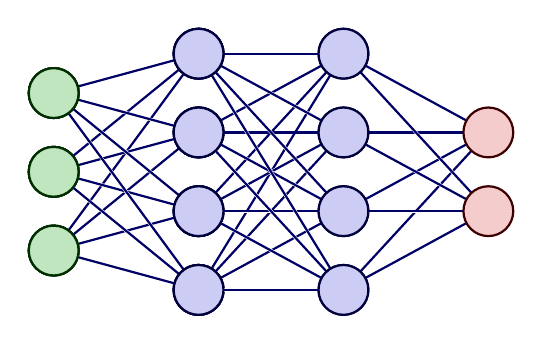
\begin{tikzpicture}[x=2.3cm,y=1.0cm]
  \message{^^JNeural network large}
  \readlist\Nnod{3,4,4,2} % array of number of nodes per layer
  
  \message{^^J  Layer}
  \foreachitem \N \in \Nnod{ % loop over layers
    \def\lay{\Ncnt} % alias of index of current layer
    \pgfmathsetmacro\prev{int(\Ncnt-1)} % number of previous layer
    \message{\lay,}
    \foreach \i [evaluate={\y=\N/2-\i; \x=\lay*0.8; \n=\nstyle;
                           \nprev=int(\prev<\Nnodlen?min(2,\prev):3);}] in {1,...,\N}{ % loop over nodes
      
      % NODES
      %\node[node \n,outer sep=0.6,minimum size=18] (N\lay-\i) at (\x,\y) {};
      \coordinate (N\lay-\i) at (\x,\y);
      
      % CONNECTIONS
      \ifnum\lay>1 % connect to previous layer
        \foreach \j in {1,...,\Nnod[\prev]}{ % loop over nodes in previous layer
          \draw[connect,white,line width=1.2] (N\prev-\j) -- (N\lay-\i);
          \draw[connect] (N\prev-\j) -- (N\lay-\i);
          %\draw[connect] (N\prev-\j.0) -- (N\lay-\i.180); % connect to left
          \node[node \nprev,minimum size=18] at (N\prev-\j) {}; % draw node over lines
        }
        \ifnum \lay=\Nnodlen % draw last node over lines
          \node[node \n,minimum size=18] at (N\lay-\i) {};
        \fi
      \fi % else: nothing to connect first layer
      
    }
  }
  
\end{tikzpicture}
        \caption{\textbf{Regular neural network:}}
        \label{subfig:cm_dt}
    \end{subfigure}
    \hfill
   \begin{subfigure}[t]{0.49\textwidth}
       \centering
       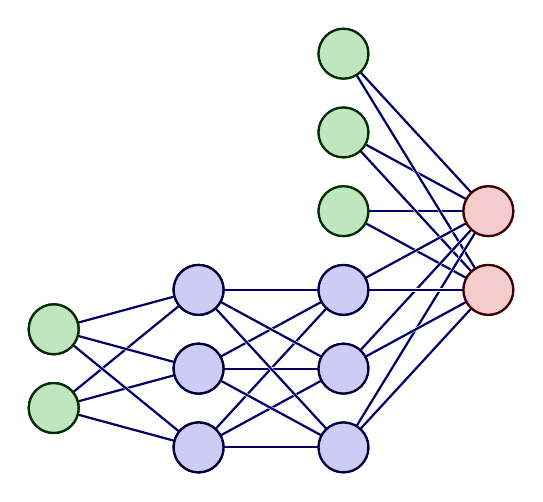
\begin{tikzpicture}[x=2.3cm,y=2.0cm]
  \message{^^JNeural network large}
  \readlist\Nnod{3,2} % array of number of nodes per layer
  \readlist\Nnodtwo{2,3,3,2}
  \message{^^J  Layer}
  \foreachitem \N \in \Nnod{ % loop over layers
    \def\lay{\Ncnt} % alias of index of current layer
    \pgfmathsetmacro\prev{int(\Ncnt-1)} % number of previous layer
    \message{\lay,}
    \foreach \i [evaluate={\y=\N/4-\i*0.5; \x=\lay*0.8+1.6; \n=\nstyle;
                           \nprev=int(\prev<\Nnodlen?min(2,\prev):3);}] in {1,...,\N}{ % loop over nodes
      
      % NODES
      %\node[node \n,outer sep=0.6,minimum size=18] (N\lay-\i) at (\x,\y) {};
      \ifnum \lay<\Nnodlen % draw last node over lines
        \coordinate (N\lay-\i) at (\x,\y);
      \else
        \coordinate (N\lay-\i) at (\x,\y-0.75);
      \fi
      % CONNECTIONS
      \ifnum\lay>1 % connect to previous layer
        \foreach \j in {1,...,\Nnod[\prev]}{ % loop over nodes in previous layer
          \draw[connect,white,line width=1.2] (N\prev-\j) -- (N\lay-\i);
          \draw[connect] (N\prev-\j) -- (N\lay-\i);
          %\draw[connect] (N\prev-\j.0) -- (N\lay-\i.180); % connect to left
          \node[node \nprev,minimum size=18] at (N\prev-\j) {}; % draw node over lines
        }
        \ifnum \lay=\Nnodlen % draw last node over lines
          \node[node \n,minimum size=18] at (N\lay-\i) {};
        \fi
      \fi % else: nothing to connect first layer
      
    }
  }

  \foreachitem \N \in \Nnodtwo{ % loop over layers
    \def\lay{\Ncnt} % alias of index of current layer
    \pgfmathsetmacro\prev{int(\Ncnt-1)} % number of previous layer
    \message{\lay,}
    \foreach \i [evaluate={\y=\N/4-\i*0.5-1.5; \x=\lay*0.8; \n=\nstyle;
                           \nprev=int(\prev<\Nnodtwolen?min(2,\prev):3);}] in {1,...,\N}{ % loop over nodes
      % NODES
      %\node[node \n,outer sep=0.6,minimum size=18] (N\lay-\i) at (\x,\y) {};
      \ifnum \lay<\Nnodtwolen % draw last node over lines
        \coordinate (M\lay-\i) at (\x,\y);
      \else
        \coordinate (M\lay-\i) at (\x,\y+0.75);
      \fi
      % CONNECTIONS
      \ifnum\lay>1 % connect to previous layer
        \foreach \j in {1,...,\Nnodtwo[\prev]}{ % loop over nodes in previous layer
          \draw[connect,white,line width=1.2] (M\prev-\j) -- (M\lay-\i);
          \draw[connect] (M\prev-\j) -- (M\lay-\i);
          %\draw[connect] (N\prev-\j.0) -- (N\lay-\i.180); % connect to left
          \node[node \nprev,minimum size=18] at (M\prev-\j) {}; % draw node over lines
        }
        \ifnum \lay=\Nnodtwolen % draw last node over lines
          \node[node \n,minimum size=18] at (M\lay-\i) {};
        \fi
      \fi % else: nothing to connect first layer
      
    }
  }
  
\end{tikzpicture}
       \caption{\textbf{Neural network with separated features 1:} Geometric and harmonic features are connected directly to the output layer}
       \label{subfig:cm_rf}
\end{subfigure}
\\~\\
    \begin{subfigure}[t]{0.49\textwidth}
        \centering
        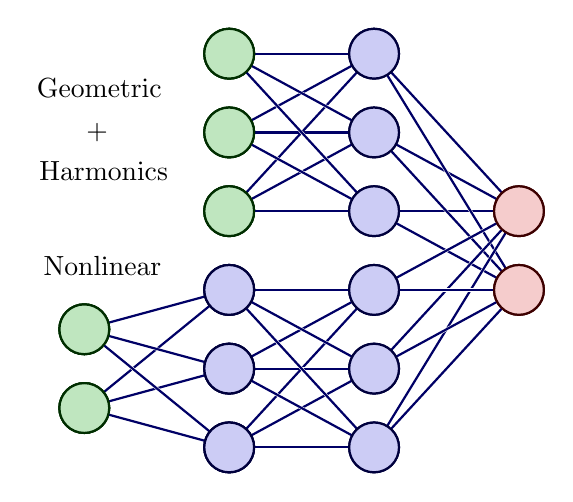
\begin{tikzpicture}[x=2.3cm,y=2.0cm]
  \message{^^JNeural network large}
  \readlist\Nnod{3,3,2} % array of number of nodes per layer
  \readlist\Nnodtwo{2,3,3,2}
  \message{^^J  Layer}
  \foreachitem \N \in \Nnod{ % loop over layers
    \def\lay{\Ncnt} % alias of index of current layer
    \pgfmathsetmacro\prev{int(\Ncnt-1)} % number of previous layer
    \message{\lay,}
    \foreach \i [evaluate={\y=\N/4-\i*0.5; \x=\lay*0.8+0.8; \n=\nstyle;
                           \nprev=int(\prev<\Nnodlen?min(2,\prev):3);}] in {1,...,\N}{ % loop over nodes
      
      % NODES
      %\node[node \n,outer sep=0.6,minimum size=18] (N\lay-\i) at (\x,\y) {};
      \ifnum \lay<\Nnodlen % draw last node over lines
        \coordinate (N\lay-\i) at (\x,\y);
      \else
        \coordinate (N\lay-\i) at (\x,\y-0.75);
      \fi
      % CONNECTIONS
      \ifnum\lay>1 % connect to previous layer
        \foreach \j in {1,...,\Nnod[\prev]}{ % loop over nodes in previous layer
          \draw[connect,white,line width=1.2] (N\prev-\j) -- (N\lay-\i);
          \draw[connect] (N\prev-\j) -- (N\lay-\i);
          %\draw[connect] (N\prev-\j.0) -- (N\lay-\i.180); % connect to left
          \node[node \nprev,minimum size=18] at (N\prev-\j) {}; % draw node over lines
        }
        \ifnum \lay=\Nnodlen % draw last node over lines
          \node[node \n,minimum size=18] at (N\lay-\i) {};
        \fi
      \fi % else: nothing to connect first layer
      
    }
  }
  \node[shift = {(-1.5,0)}] at (N2-2){
    $\begin{aligned}
      \text{Geom}&\text{etric}\\
      +&\\
      \text{Harm}&\text{onics}
    \end{aligned}$
  };
  \node[shift = {(-1.5,-0.85)}] at (N2-2){Nonlinear};
  \foreachitem \N \in \Nnodtwo{ % loop over layers
    \def\lay{\Ncnt} % alias of index of current layer
    \pgfmathsetmacro\prev{int(\Ncnt-1)} % number of previous layer
    \message{\lay,}
    \foreach \i [evaluate={\y=\N/4-\i*0.5-1.5; \x=\lay*0.8; \n=\nstyle;
                           \nprev=int(\prev<\Nnodtwolen?min(2,\prev):3);}] in {1,...,\N}{ % loop over nodes
      % NODES
      %\node[node \n,outer sep=0.6,minimum size=18] (N\lay-\i) at (\x,\y) {};
      \ifnum \lay<\Nnodtwolen % draw last node over lines
        \coordinate (M\lay-\i) at (\x,\y);
      \else
        \coordinate (M\lay-\i) at (\x,\y+0.75);
      \fi
      % CONNECTIONS
      \ifnum\lay>1 % connect to previous layer
        \foreach \j in {1,...,\Nnodtwo[\prev]}{ % loop over nodes in previous layer
          \draw[connect,white,line width=1.2] (M\prev-\j) -- (M\lay-\i);
          \draw[connect] (M\prev-\j) -- (M\lay-\i);
          %\draw[connect] (N\prev-\j.0) -- (N\lay-\i.180); % connect to left
          \node[node \nprev,minimum size=18] at (M\prev-\j) {}; % draw node over lines
        }
        \ifnum \lay=\Nnodtwolen % draw last node over lines
          \node[node \n,minimum size=18] at (M\lay-\i) {};
        \fi
      \fi % else: nothing to connect first layer
      
    }
  }
  
\end{tikzpicture}
        \caption{\textbf{Neural network with separated features 2}: Geometric and harmonic features are separated from the other features, but also processed by a nonlinear activation function.}
        \label{subfig:cm_bag}
    \end{subfigure}
    \hfill
       \begin{subfigure}[t]{0.49\textwidth}
        \centering
        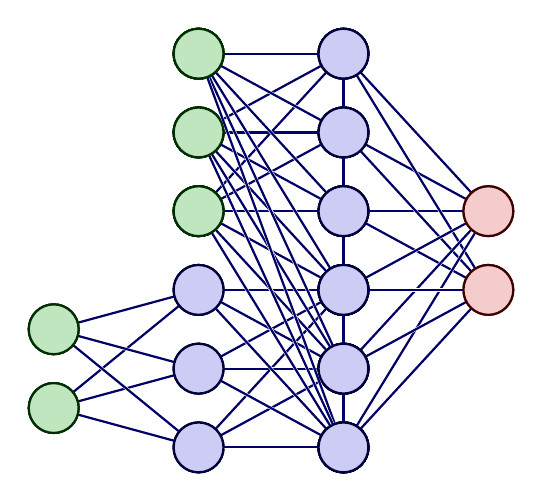
\begin{tikzpicture}[x=2.3cm,y=2.0cm]
  \message{^^JNeural network large}
  \readlist\Nnod{3,3,2} % array of number of nodes per layer
  \readlist\Nnodtwo{2,3,3,2}
  \message{^^J  Layer}
  \foreachitem \N \in \Nnod{ % loop over layers
    \def\lay{\Ncnt} % alias of index of current layer
    \pgfmathsetmacro\prev{int(\Ncnt-1)} % number of previous layer
    \message{\lay,}
    \foreach \i [evaluate={\y=\N/4-\i*0.5; \x=\lay*0.8+0.8; \n=\nstyle;
                           \nprev=int(\prev<\Nnodlen?min(2,\prev):3);}] in {1,...,\N}{ % loop over nodes
      
      % NODES
      %\node[node \n,outer sep=0.6,minimum size=18] (N\lay-\i) at (\x,\y) {};
      \ifnum \lay<\Nnodlen % draw last node over lines
        \coordinate (N\lay-\i) at (\x,\y);
      \else
        \coordinate (N\lay-\i) at (\x,\y-0.75);
      \fi
      % CONNECTIONS
      \ifnum\lay>1 % connect to previous layer
        \foreach \j in {1,...,\Nnod[\prev]}{ % loop over nodes in previous layer
          \draw[connect,white,line width=1.2] (N\prev-\j) -- (N\lay-\i);
          \draw[connect] (N\prev-\j) -- (N\lay-\i);
          %\draw[connect] (N\prev-\j.0) -- (N\lay-\i.180); % connect to left
          \node[node \nprev,minimum size=18] at (N\prev-\j) {}; % draw node over lines
        }
        \ifnum \lay=\Nnodlen % draw last node over lines
          \node[node \n,minimum size=18] at (N\lay-\i) {};
        \fi
      \fi % else: nothing to connect first layer
      
    }
  }

  \foreachitem \N \in \Nnodtwo{ % loop over layers
    \def\lay{\Ncnt} % alias of index of current layer
    \pgfmathsetmacro\prev{int(\Ncnt-1)} % number of previous layer
    \message{\lay,}
    \foreach \i [evaluate={\y=\N/4-\i*0.5-1.5; \x=\lay*0.8; \n=\nstyle;
                           \nprev=int(\prev<\Nnodtwolen?min(2,\prev):3);}] in {1,...,\N}{ % loop over nodes
      % NODES
      %\node[node \n,outer sep=0.6,minimum size=18] (N\lay-\i) at (\x,\y) {};
      \ifnum \lay<\Nnodtwolen % draw last node over lines
        \coordinate (M\lay-\i) at (\x,\y);
      \else
        \coordinate (M\lay-\i) at (\x,\y+0.75);
      \fi
      % CONNECTIONS
      \ifnum\lay>1 % connect to previous layer
        \foreach \j in {1,...,\Nnodtwo[\prev]}{ % loop over nodes in previous layer
          \draw[connect,white,line width=1.2] (M\prev-\j) -- (M\lay-\i);
          \draw[connect] (M\prev-\j) -- (M\lay-\i);
          %\draw[connect] (N\prev-\j.0) -- (N\lay-\i.180); % connect to left
          \node[node \nprev,minimum size=18] at (M\prev-\j) {}; % draw node over lines
        }
        \ifnum \lay=\Nnodtwolen % draw last node over lines
          \node[node \n,minimum size=18] at (M\lay-\i) {};
        \fi
      \fi % else: nothing to connect first layer
      
    }
  }

  \foreachitem \N \in \Nnod{ % loop over layers
    \def\lay{\Ncnt} % alias of index of current layer
    \pgfmathsetmacro\prev{int(\Ncnt-1)} % number of previous layer
    \message{\lay,}
    \foreach \i [evaluate={\y=\N-\i*0.5; \x=\lay; \n=\nstyle;
                           \nprev=int(\prev<\Nnodlen?min(2,\prev):3);}] in {1,...,\N}{ % loop over nodes
      
      % CONNECTIONS
      \ifnum\lay=2 % connect to previous layer
        \foreach \j in {1,...,\Nnod[\prev]}{ % loop over nodes in previous layer
          \draw[connect,white,line width=1.2] (M3-\j) -- (N\lay-\i);
          \draw[connect] (M3-\j) -- (N\lay-\i);
          %\draw[connect] (N\prev-\j.0) -- (N\lay-\i.180); % connect to left
          \message{^^J Nprev \nprev}
          \node[node 2,minimum size=18] at (M3-\j) {}; % draw node over lines
          \node[node 2,minimum size=18] at (N\lay-\j) {}; % draw node over lines
        }
      \fi % else: nothing to connect first layer
      
    }
  }

  \foreachitem \N \in \Nnodtwo{ % loop over layers
    \def\lay{\Ncnt} % alias of index of current layer
    \pgfmathsetmacro\prev{int(\Ncnt-1)} % number of previous layer
    \message{\lay,}
    \foreach \i [evaluate={\y=\N/4-\i*0.5; \x=\lay+2; \n=\nstyle;
                           \nprev=int(\prev<\Nnodtwolen?min(2,\prev):3);}] in {1,...,\N}{ % loop over nodes
      % NODES
      %\node[node \n,outer sep=0.6,minimum size=18] (N\lay-\i) at (\x,\y) {};
      \ifnum\lay=3 % connect to previous layer
        \foreach \j in {1,...,\Nnodtwo[\prev]}{ % loop over nodes in previous layer
          \message{^^J \lay Here (N1-\j) {l\lay}}
          \draw[connect,white,line width=1.2] (N1-\j) -- (M\lay-\i);
          \draw[connect] (N1-\j) -- (M\lay-\i);
          %\draw[connect] (N\prev-\j.0) -- (N\lay-\i.180); % connect to left
          \node[node 1,minimum size=18] at (N1-\j) {}; % draw node over lines
          \node[node 2,minimum size=18] at (M\lay-\j) {}; % draw node over lines
          
        }

      \fi % else: nothing to connect first layer
      
    }
  }



\end{tikzpicture}
        \caption{\textbf{Neural network with separated features 3:} Processed regular features are concatenated with geometric and harmonic features.}
        \label{subfig:cm_bos}
    \end{subfigure}
     \caption{Neural network architecture for the base pointing model trained on raw data.}
     \label{fig:nn_architecture}
\end{figure}

The hyperparameters for the neural networks were sampled from different distributions, as presented in Table \ref{tab:nn_hyperparameters}.
While some parameters were consistent across all models, such as the use of the Adam optimization algorithm, and the mean squared error loss function.



\begin{table}[H]
    \centering
    \caption{This table presents a list of parameters that are sampled during hyperparameter tuning for the base pointing model. The table includes names, distributions that are sampled from, and corresponding ranges.}
    \begin{tabular}{lcc}
    \hline
    \textbf{Name} & \textbf{Distribution Type} & \textbf{Range} \\ \hline
    hidden layers & uniform integer & [1,3] \\
    hidden layer size & uniform integer & [20, 120] \\
    learning rate & uniform & [0.001, 0.02] \\
    batch size & uniform integer & [32, 512] \\
    activation & categorical & [gelu, tanh] \\ \hline
    \end{tabular}
    \label{tab:nn_hyperparameters}
    \end{table}
\subsection{Model Evaluation}

\section{Experiment 2: Pointing Correction Model}
In this experiment, we aim to improve the pointing accuracy by training XGBoost models to predict offsets obtained by pointing scans.
We use four different datasets, all of which are preprocessed using our cleaning criteria and the XGBoost classifier trained to remove bad pointing scans.
These datasets use
\begin{itemize}
\item all instruments
\item NFLASH230 only
\item all instruments transformed to simulate optimal pointing corrections
\item NFLASH230 only transformed to simulate optimal pointing corrections
\end{itemize}

By training our models on these datasets, we hope to reduce the pointing offset and improve the accuracy of the pointing.

In addition, we varied the way we split the datasets for training and testing.
We considered two cases:

\begin{itemize}
    \item \textbf{Case 1:} The dataset is sorted by date and split into six equal-sized folds.
    We consider each of the folds one by one.
    For each of these folds, we use the last $1/6$th of the data set test, and the remaining $5/6$th as training and validation.
    \item \textbf{Case 2:} The dataset is sorted by date and split into six equal-sized folds.
    We used $5/6$ of the data for training and validation and the remaining for testing.
    We repeated this process six times, using each fold for testing once.
\end{itemize}

Figure \ref{fig:datasplit_cases} illustrates the two cases.
In both cases, we trained and validated the model on $5/6$ of the data and tested on the last $1/6$.
The difference is the amount of data used for training, which can indicate whether models trained on shorter or longer periods perform better.

\begin{figure}[H]
    \centering
    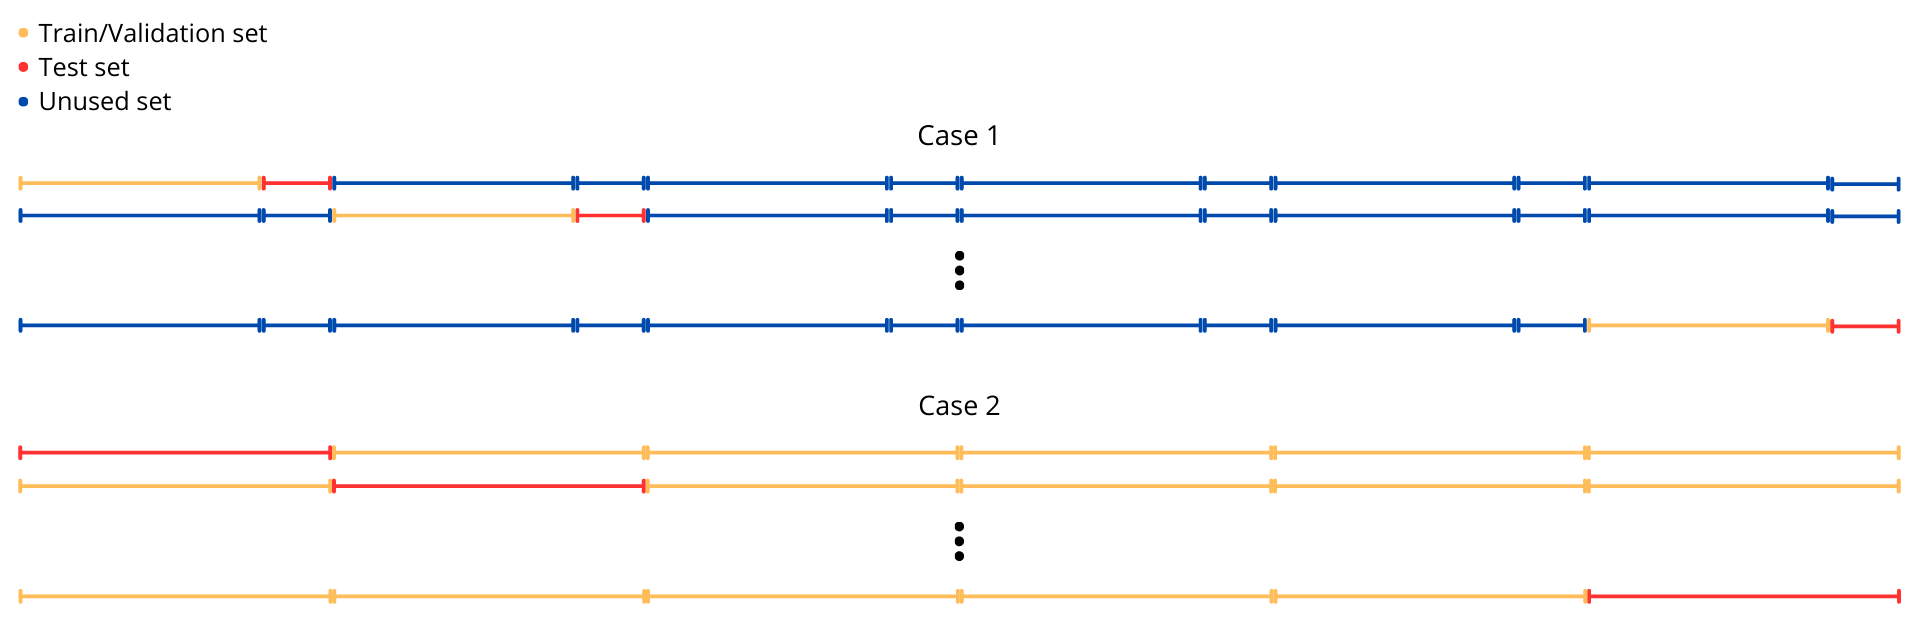
\includegraphics[width=0.98\textwidth]{Canva/datasplits.png}
    \caption{Two cross-validation cases are shown, where the orange region represents the train and validation set, the red region represents the test set, and the blue region is unused for evaluation.
    In \textbf{Case 1}, the dataset is split into six equal-sized folds sorted by date.
    For the selected fold, the last part (colored red) is used for testing, and the remaining part (colored orange) is used for training and validation.
    This process is repeated six times, once for each fold.
    In \textbf{Case 2}, the dataset is again split into six equal-sized folds sorted by date.
    However, this time, one whole fold is used for testing, and the remaining five folds are used for training and validation.
    This process is repeated six times, with each fold used exactly once for testing.}
    \label{fig:datasplit_cases}
\end{figure}




\subsection{Feature Selection}
We trained models using a range of features, specifically $k=[2,5,10,20,30,40,50]$ features.
For each model, we selected the $k$ features that had the greatest mutual information with the target value.
This approach helps us identify the most important features and can improve the model's performance by reducing overfitting and noise.
By selecting different numbers of features, we can explore the trade-off between model complexity and performance.\textcolor{red}{write and ref to mutual info in theory section}.

\subsection{Model Architecture}
For each model, we performed a Bayesian hyperparameter search using the parameter space shown in Table \ref{tab:xgb_hyperparameters_pcorr}.
The search space includes eight hyperparameters that affect the model's complexity, such as the maximum depth of the trees, the regularization strength, and the learning rate.
We used a uniform or log-uniform distribution to sample each hyperparameter within a specific range.
In total, we evaluated $200$ different combinations of hyperparameters (for each dataset, cross-validation case, target variable, and the number of features selected) to find the optimal values for each model.
The models were validated using the MSE, and the model with the best performance on the validation set was picked.


\begin{table}[H]
    \centering
    \caption{This table presents a list of parameters that are sampled during hyperparameter tuning for the pointing correction model. The table includes names, distributions that are sampled from, and corresponding ranges.}
    \begin{tabular}{lcc}
        \hline
        \textbf{Parameter} & \textbf{Sample Distribution} & \textbf{Range} \\ \hline
        max depth & Uniform & [1, 5] \\ 
        reg lambda & Uniform & [0, 1] \\ 
        colsample bytree & Uniform & [0.5, 1] \\ 
        n estimators & Uniform & [20, 500] \\ 
        learning rate & Log-Uniform & [$10^{-5}$, 1] \\ 
        subsample & Uniform & [0.5, 1] \\ 
        gamma & Log-Uniform & [$10^{-5}$, 1] \\ 
        min child weight & Uniform & [1, 10] \\ 
    \end{tabular}
    \label{tab:xgb_hyperparameters_pcorr}
\end{table}



\subsection{Model Evaluation}
To evaluate the performance of the models, we calculated the RMS on each test fold and compared it to the current RMS of the telescope on the same data.
We then computed the ratio of the model's RMS to the current RMS for each fold, denoted as $r_{RMS,i}$.
If the ratio is less than $1$, it indicates that the XGBoost model provides an improvement over the current performance of the telescope on that fold.

To obtain an overall measure of the model's performance compared to the current performance of the telescope, we averaged the ratios $r_{RMS,i}$ over all six test folds
\begin{equation}
    \bar{r}_{RMS} = \sum_{i=1}^6 \frac{RMS_{model,i}}{RMS_{current,i}}.
\end{equation}
This gives us an average ratio denoted as $\bar{r}_{RMS}$, which is a measure of the improvement in performance provided by the XGBoost model.
If $\bar{r}_{RMS} < 1$, it indicates that the XGBoost model outperforms the current pointing correction method on average across all test folds.
By comparing the average ratio $\bar{r}_{RMS}$ for the two different cross-validation cases and the selected number of features, we can identify which models provide the best performance.

\chapter{Results}

\chapter{Discussion}

\chapter{Conclusion}

\pagestyle{plain}
\appendix
\chapter*{Appendices}
\section*{Appendix A}
\section{Pointing Correction Results}

\begin{table}[h]
    \centering %$tmp2022\_clean\_clf\_nflash230\_results\_table$
    \caption{Resulting RMS from Case $1$ and $2$ for XGBoost model predicting pointing offset.
    The dataset used to get these results contains only data from NFLASH230 and is cleaned using the regular criteria and XGBoost classifier.}
    \begin{tabular}{ccc c cc}
        \toprule
        \multicolumn{1}{c}{} & \multicolumn{2}{c}{RMS Case 1} & & \multicolumn{2}{c}{RMS Case 2} \\
        \cmidrule(lr){2-3} \cmidrule(lr){5-6}
        k & Azimuth & Elevation & & Azimuth & Elevation \\
        \midrule
        2 &  0.983957 &  1.018378 & &  0.926561 &  0.991728 \\
        5 &  1.297720 &  1.137682 & &  0.938401 &  0.987364 \\
       10 &  1.428557 &  1.153950 & &  0.966462 &  1.002820 \\
       20 &  1.229440 &  1.103770 & &  0.943179 &  0.984103 \\
       30 &  1.387079 &  1.064364 & &  0.958910 &  0.995761 \\
       40 &  1.224572 &  1.054826 & &  0.962620 &  1.004978 \\
       50 &  1.179139 &  1.073336 & &  0.974661 &  0.968089 \\
        \bottomrule
    \end{tabular}
\end{table}


\begin{table}[h]
    \centering %$tmp2022\_clean\_clf\_nflash230\_transformed\_results\_table$
    \caption{Resulting RMS from Case $1$ and $2$ for XGBoost model predicting pointing offset.
    The dataset used to get these results contains only data from NFLASH230 and is cleaned using the regular criteria and XGBoost classifier.
    are transformed to simulate a pointing correction after every scan.}
    \begin{tabular}{ccc c cc}
        \toprule
        \multicolumn{1}{c}{} & \multicolumn{2}{c}{RMS Case 1} & & \multicolumn{2}{c}{RMS Case 2} \\
        \cmidrule(lr){2-3} \cmidrule(lr){5-6}
        k & Azimuth & Elevation & & Azimuth & Elevation \\
        \midrule
        2 &  1.063771 &  1.097368 & &  0.982346 &  1.023116 \\
        5 &  1.158891 &  1.135054 & &  0.974600 &  1.005169 \\
       10 &  1.110609 &  1.074162 & &  0.989497 &  1.005604 \\
       20 &  1.125938 &  1.001437 & &  0.970074 &  1.013085 \\
       30 &  1.126540 &  1.023054 & &  0.994982 &  0.971606 \\
       40 &  1.134314 &  1.065193 & &  1.013492 &  1.041213 \\
       50 &  1.112269 &  1.028447 & &  0.980788 &  0.998984 \\
       \bottomrule
        \bottomrule
    \end{tabular}
\end{table}

\begin{table}[h]
    \centering %$tmp2022\_clean\_clf\_results\_table$
    \caption{Resulting RMS from Case $1$ and $2$ for XGBoost model predicting pointing offset.
    The dataset used to get these results contain all scans and is cleaned using the regular criteria and the XGBoost classifier.}
    \begin{tabular}{ccc c cc}
        \toprule
        \multicolumn{1}{c}{} & \multicolumn{2}{c}{RMS Case 1} & & \multicolumn{2}{c}{RMS Case 2} \\
        \cmidrule(lr){2-3} \cmidrule(lr){5-6}
         k & Azimuth & Elevation & & Azimuth & Elevation \\
        \midrule
        2 &  1.005252 &  1.232152 & &  0.963643 &  0.966159 \\
        5 &  1.002968 &  1.228990 & &  0.962584 &  0.952695 \\
       10 &  1.289085 &  1.212770 & &  0.969236 &  0.983188 \\
       20 &  1.474769 &  1.223286 & &  0.973215 &  0.957379 \\
       30 &  1.420438 &  1.217082 & &  0.977044 &  0.957553 \\
       40 &  1.359452 &  1.250011 & &  0.981884 &  0.939400 \\
       50 &  1.447718 &  1.239426 & &  0.960710 &  0.950992 \\
        \bottomrule
    \end{tabular}
\end{table}

\begin{table}[h]
    \centering %$tmp2022\_clean\_clf\_transformed\_results\_table$
    \caption{Resulting RMS from Case $1$ and $2$ for XGBoost model predicting pointing offset.
    The dataset used to get these results contain all scans and is cleaned using the regular criteria and the XGBoost classifier.
    It is also transformed to simulate a pointing correction after every scan.}
    \begin{tabular}{ccc c cc}
        \toprule
        \multicolumn{1}{c}{} & \multicolumn{2}{c}{RMS Case 1} & & \multicolumn{2}{c}{RMS Case 2} \\
        \cmidrule(lr){2-3} \cmidrule(lr){5-6}
        k & Azimuth & Elevation & & Azimuth & Elevation \\
        \midrule
        2 &  1.411340 &  1.072811 & &  0.958876 &  0.944501 \\
        5 &  1.658062 &  1.095572 & &  0.959785 &  0.959705 \\
       10 &  1.656576 &  1.144753 & &  0.977446 &  0.943979 \\
       20 &  1.744980 &  1.020705 & &  0.974366 &  0.946778 \\
       30 &  1.891196 &  1.006098 & &  0.998285 &  0.940884 \\
       40 &  2.040398 &  0.993940 & &  0.972515 &  0.952763 \\
       50 &  2.226176 &  0.997667 & &  0.976921 &  0.942357 \\
    \bottomrule
\end{tabular}
\end{table}
%%%%%%%%%%%%%%%%%%%%%%% SPLIT ON DAYS BELOW
\begin{table}[h]
    \centering %$tmp2022\_clean\_clf\_nflash230\_results\_table$
    \caption{Resulting RMS from Case $1$ and $2$ for XGBoost model predicting pointing offset.
    The dataset used to get these results contain only NFLASH230 and is cleaned using the regular criteria and the XGBoost classifier.
    The training and validation data is split on days, meaning that all the scans for a given day
    are in the training or validation set and not both. The test set is unaffected by this.}
    \begin{tabular}{ccc c cc}
        \toprule
        \multicolumn{1}{c}{} & \multicolumn{2}{c}{RMS Case 1} & & \multicolumn{2}{c}{RMS Case 2} \\
        \cmidrule(lr){2-3} \cmidrule(lr){5-6}
         k & Azimuth & Elevation & & Azimuth & Elevation \\
        \midrule
        2 &  0.982285 &  1.019755 & &  0.929712 &  0.956510 \\
        5 &  1.365704 &  1.198440 & &  0.917298 &  0.937182 \\
       10 &  1.383077 &  1.155258 & &  0.951214 &  0.943254 \\
       20 &  1.251918 &  1.126138 & &  0.939914 &  0.942015 \\
       30 &  1.334676 &  1.093938 & &  0.928257 &  0.939238 \\
       40 &  1.145716 &  1.057689 & &  0.936151 &  0.955285 \\
       50 &  1.201661 &  1.061612 & &  0.937422 &  0.941564 \\
        \bottomrule
    \end{tabular}
\end{table}


\begin{table}[h]
    \centering
    \caption{Resulting RMS from Case $1$ and $2$ for XGBoost model predicting pointing offset.
    The dataset used to get these results contain only NFLASH230 and is cleaned using the regular criteria and the XGBoost classifier.
    It is also transformed to simulate a pointing correction after every scan.
    $tmp2022\_clean\_clf\_nflash230\_transformed\_results\_table$,
    The training and validation data is split on days, meaning that all the scans for a given day
    are in the training or validation set and not both. The test set is unaffected by this.}
    \begin{tabular}{ccc c cc}
        \toprule
        \multicolumn{1}{c}{} & \multicolumn{2}{c}{RMS Case 1} & & \multicolumn{2}{c}{RMS Case 2} \\
        \cmidrule(lr){2-3} \cmidrule(lr){5-6}
         k & Azimuth & Elevation & & Azimuth & Elevation \\
        \midrule
        2 &  1.030842 &  1.005132 & &  0.982900 &  1.057857 \\
        5 &  1.036558 &  1.000412 & &  0.983725 &  1.031629 \\
       10 &  1.136567 &  1.008504 & &  0.987074 &  1.012463 \\
       20 &  1.042592 &  1.008786 & &  0.977380 &  0.994046 \\
       30 &  1.242498 &  1.004090 & &  0.977887 &  1.008825 \\
       40 &  1.214723 &  1.006611 & &  1.006974 &  0.996165 \\
       50 &  1.180379 &  0.992092 & &  0.983166 &  0.976880 \\
        \bottomrule
    \end{tabular}
\end{table}

\begin{table}[h]
    \centering %$tmp2022\_clean\_clf\_results\_table$
    \caption{Resulting RMS from Case $1$ and $2$ for XGBoost model predicting pointing offset.
    The dataset used to get these results contain all scans and is cleaned using the regular criteria and the XGBoost classifier.
    The training and validation data is split on days, meaning that all the scans for a given day
    are in the training or validation set and not both. The test set is unaffected by this.}
    \begin{tabular}{ccc c cc}
        \toprule
        \multicolumn{1}{c}{} & \multicolumn{2}{c}{RMS Case 1} & & \multicolumn{2}{c}{RMS Case 2} \\
        \cmidrule(lr){2-3} \cmidrule(lr){5-6}
         k & Azimuth & Elevation & & Azimuth & Elevation \\
        \midrule
        2 &  1.007153 &  1.232004 & &  0.959771 &  0.957618 \\
        5 &  1.002580 &  1.169598 & &  0.955311 &  0.967055 \\
       10 &  1.287770 &  1.115745 & &  0.957866 &  0.962132 \\
       20 &  1.579776 &  1.120837 & &  0.969443 &  0.957544 \\
       30 &  1.606464 &  1.107195 & &  0.967436 &  0.971148 \\
       40 &  1.528256 &  1.068496 & &  0.979982 &  0.951577 \\
       50 &  1.757519 &  1.061275 & &  0.993239 &  0.947433 \\
        \bottomrule
    \end{tabular}
\end{table}

\begin{table}[h]
    \centering %$tmp2022\_clean\_clf\_transformed\_results\_table$
    \caption{Resulting RMS from Case $1$ and $2$ for XGBoost model predicting pointing offset.
    The dataset used to get these results contain all scans and is cleaned using the regular criteria and the XGBoost classifier.
    It is also transformed to simulate a pointing correction after every scan.
    The training and validation data is split on days, meaning that all the scans for a given day
    are in the training or validation set and not both. The test set is unaffected by this.}
    \begin{tabular}{ccc c cc}
        \toprule
        \multicolumn{1}{c}{} & \multicolumn{2}{c}{RMS Case 1} & & \multicolumn{2}{c}{RMS Case 2} \\
        \cmidrule(lr){2-3} \cmidrule(lr){5-6}
         k & Azimuth & Elevation & & Azimuth & Elevation \\
        \midrule
        2 &  1.362174 &  1.049563 & &  0.958867 &  0.949895 \\
        5 &  1.519794 &  1.073077 & &  0.968773 &  0.951299 \\
       10 &  1.515574 &  1.043983 & &  0.974003 &  0.948826 \\
       20 &  1.698061 &  1.017496 & &  0.981890 &  0.939138 \\
       30 &  1.716675 &  1.014389 & &  0.979207 &  0.957982 \\
       40 &  2.476614 &  1.034294 & &  0.990171 &  0.947986 \\
       50 &  2.493252 &  1.031271 & &  0.968949 &  0.943721 \\
        \bottomrule
    \end{tabular}        
\end{table}


\section{Raw data correlation}
\begin{table}[h]
    \centering %$tmp2022\_clean\_clf\_transformed\_results\_table$
    \caption{Features with Spearman's rank correlation $\geq 0.1$ to either one of the target values.}
    \begin{tabular}{lccc}
        \toprule
        Feature &  $\delta_{\text{Az}}$ &  $\delta_{\text{El}}$ &  $\delta_{\text{Az}}\cos{\text{El}}$ \\
        \midrule
        WINDSPEED\_VAR\_5        &      $0.10$ &      $0.12$ &               $0.11$ \\
        DAZ\_TILT\_MEDIAN\_1      &      $0.09$ &      $0.03$ &               $0.14$ \\
        DAZ\_TILTTEMP\_MEDIAN\_1  &      $0.00$ &     -$0.06$ &               $0.30$ \\
        TILT1Y\_MEDIAN\_1        &      $0.08$ &      $0.02$ &               $0.13$ \\
        TEMP26\_MEDIAN\_1        &      $0.06$ &      $0.13$ &              $-0.19$ \\
        TEMP27\_MEDIAN\_1        &      $0.06$ &      $0.13$ &              $-0.21$ \\
        TEMP28\_MEDIAN\_1        &      $0.04$ &      $0.11$ &              $-0.25$ \\
        TEMPERATURE\_MEDIAN\_1   &      $0.04$ &      $0.12$ &              $-0.26$ \\
        POSITIONZ\_MEDIAN\_1     &      $0.05$ &      $0.11$ &              $-0.21$ \\
        DEWPOINT\_MEDIAN\_1      &      $0.08$ &      $0.12$ &              $-0.15$ \\
        DAZ\_TOTAL\_MEDIAN\_1     &      $0.09$ &      $0.03$ &               $0.13$ \\
        WINDSPEED\_MEDIAN\_1     &      $0.02$ &      $0.02$ &               $0.13$ \\
        HESE2                  &      $0.46$ &      $0.44$ &               $0.44$ \\
        HESE3                  &      $0.98$ &      $0.94$ &               $0.77$ \\
        HESE4                  &      $0.97$ &      $0.92$ &               $0.74$ \\
        HESE5                  &      $0.34$ &      $0.31$ &               $0.15$ \\
        HACA5                  &      $0.06$ &      $0.05$ &               $0.10$ \\
        HECE                   &      $1.00$ &      $0.96$ &               $0.78$ \\
        HECE2                  &      $1.00$ &      $0.96$ &               $0.78$ \\
        HECE3                  &      $0.76$ &      $0.72$ &               $0.52$ \\
        HSCA5                  &      $0.12$ &      $0.11$ &               $0.14$ \\
        \bottomrule
    \end{tabular}
\end{table}

\begin{table}[h]
    \centering %$tmp2022\_clean\_clf\_transformed\_results\_table$
    \caption{Features with Pearson's correlation $\geq 0.1$ to either one of the target values.}
    \begin{tabular}{lccc}
        \toprule
        Feature &  $\delta_{\text{Az}}$ &  $\delta_{\text{El}}$ &  $\delta_{\text{Az}}\cos{\text{El}}$ \\
        \midrule
        TEMP26\_MEDIAN\_1        &      $0.05$ &      $0.11$ &              $-0.12$ \\
        TEMP27\_MEDIAN\_1        &      $0.05$ &      $0.11$ &              $-0.13$ \\
        DAZ\_TOTAL\_MEDIAN\_1     &      $0.12$ &      $0.08$ &               $0.07$ \\
        WINDSPEED\_MEDIAN\_1     &      $0.03$ &      $0.03$ &               $0.10$ \\
        AWAZ                   &      $0.00$ &     $-0.01$ &               $0.57$ \\
        HESE2                  &      $0.56$ &      $0.54$ &               $0.45$ \\
        HESE3                  &      $0.97$ &      $0.90$ &               $0.43$ \\
        HESE4                  &      $0.91$ &      $0.82$ &               $0.26$ \\
        HESE5                  &      $0.29$ &      $0.22$ &              $-0.11$ \\
        HECE                   &      $1.00$ &      $0.92$ &               $0.45$ \\
        HECE2                  &      $0.98$ &      $0.89$ &               $0.38$ \\
        HECE3                  &      $0.70$ &      $0.62$ &               $0.10$ \\
        HSCA                   &      $0.01$ &     $-0.00$ &               $0.53$ \\
        \bottomrule
        \end{tabular}
\end{table}


\section{Base pointing model results}
% \begin{table}[h]
%     \centering
%     \caption{Regular neural network}
%     \begin{tabular}{ccccccc}
%         \toprule
%         Mean & STD & Activation function & Hidden layers & Learning rate & Batch size & Loss function \\
%         18.37 & 11.88 &       Tanh &    [[22, 46]] &          0.01 &        475 & MSE \\
%         18.41 &  7.46 &       GeLU &        [[46]] &          0.01 &        472 & MSD \\
%         18.84 &  5.60 &       ReLU &        [[82]] &          0.02 &        334 & MSE \\
%         19.42 &  9.50 &       Tanh &        [[64]] &          0.01 &         61 & MSE \\
%         22.06 &  7.88 &       ReLU &        [[20]] &          0.00 &        309 & MSD \\
%         \bottomrule
%     \end{tabular}
% \end{table}


% \begin{table}[h]
%     \centering %$tmp2022\_clean\_clf\_transformed\_results\_table$
%     \caption{Resulting RMS from Case $1$ and $2$ for XGBoost model predicting pointing offset.
%     The dataset used to get these results contain all scans and is cleaned using the regular criteria and the XGBoost classifier.
%     It is also transformed to simulate a pointing correction after every scan.}
%     \begin{tabular}{ccc c cc}
%         \toprule
%         \multicolumn{1}{c}{} & \multicolumn{2}{c}{RMS Case 1} & & \multicolumn{2}{c}{RMS Case 2} \\
%         \cmidrule(lr){2-3} \cmidrule(lr){5-6}
%         k & Azimuth & Elevation & & Azimuth & Elevation \\
%         \midrule
%         2 &  1.411340 &  1.072811 & &  0.958876 &  0.944501 \\
%         5 &  1.658062 &  1.095572 & &  0.959785 &  0.959705 \\
%        10 &  1.656576 &  1.144753 & &  0.977446 &  0.943979 \\
%        20 &  1.744980 &  1.020705 & &  0.974366 &  0.946778 \\
%        30 &  1.891196 &  1.006098 & &  0.998285 &  0.940884 \\
%        40 &  2.040398 &  0.993940 & &  0.972515 &  0.952763 \\
%        50 &  2.226176 &  0.997667 & &  0.976921 &  0.942357 \\
%     \bottomrule
% \end{tabular}
% \end{table}

\begin{table}[h]
    \centering
    \caption{Separate 1}
    \begin{tabular}{ccccccc}
        \toprule
        \multicolumn{2}{c}{RMS test set} & \multicolumn{5}{c}{Hyperparameters} \\
        \cmidrule(lr){1-2} 
        Mean & STD & Activation function & Hidden layers & Learning rate & Batch size & Loss function \\
        \midrule
        17.41 &  7.87 &       Tanh &        [40] &          0.01 &        101 & MSD \\
        18.78 & 10.02 &       GeLU &   [86, 106] &          0.02 &         43 & MSD \\
        20.26 & 10.58 &       ReLU &    [68, 42] &          0.02 &        450 & MSD \\
        21.51 &  8.38 &       Tanh &        [32] &          0.02 &        266 & MSE \\
        22.14 & 11.76 &       ReLU &       [106] &          0.02 &         95 & MSE \\
        \bottomrule
    \end{tabular}
\end{table}


% \begin{table}[h]
%     \centering
%     \caption{Separate 2}
%     \begin{tabular}{rrllrrl}
%         \toprule
%         RMS Test & Activation function & Hidden layers & Learning rate & Batch size & Loss function \\
%         20.25 &  6.50 &       Tanh &        [[62]] &          0.00 &        155 & MSD \\
%         20.52 &  5.52 &       Tanh &        [[40]] &          0.01 &        101 & MSD \\
%         22.19 &  7.02 &       GeLU &        [[54]] &          0.02 &        413 & MSD \\
%         23.19 & 16.15 &       ReLU &        [[81]] &          0.01 &        439 & MSD \\
%         24.14 & 14.64 &       GeLU &    [[97, 24]] &          0.02 &        321 & MSE \\
%         \bottomrule
%     \end{tabular}
% \end{table}


% \begin{table}[h]
%     \centering
%     \caption{Separate 3}
%     \begin{tabular}{rrllrrl}
%         \toprule
%         RMS Test & Activation function & Hidden layers & Learning rate & Batch size & Loss function \\
%         17.12 &  8.42 &       Tanh &        [[26]] &          0.00 &        358 & MSD \\
%         19.10 &  7.94 &       Tanh &    [[49, 40]] &          0.02 &        320 & MSD \\
%         19.81 & 13.94 &       ReLU &    [[97, 60]] &          0.02 &        359 & MSD \\
%         19.84 & 12.64 &       ReLU &   [[117, 32]] &          0.02 &        298 & MSD \\
%         20.20 &  9.28 &       ReLU &    [[83, 32]] &          0.01 &        331 & MSD \\
%         \bottomrule
%     \end{tabular}
% \end{table}
    


\newpage

\bibliographystyle{plain} % We choose the "plain" reference style
\bibliography{citations}

\end{document}
